\section{r256} 

\subsection{dr5d5\_r256}
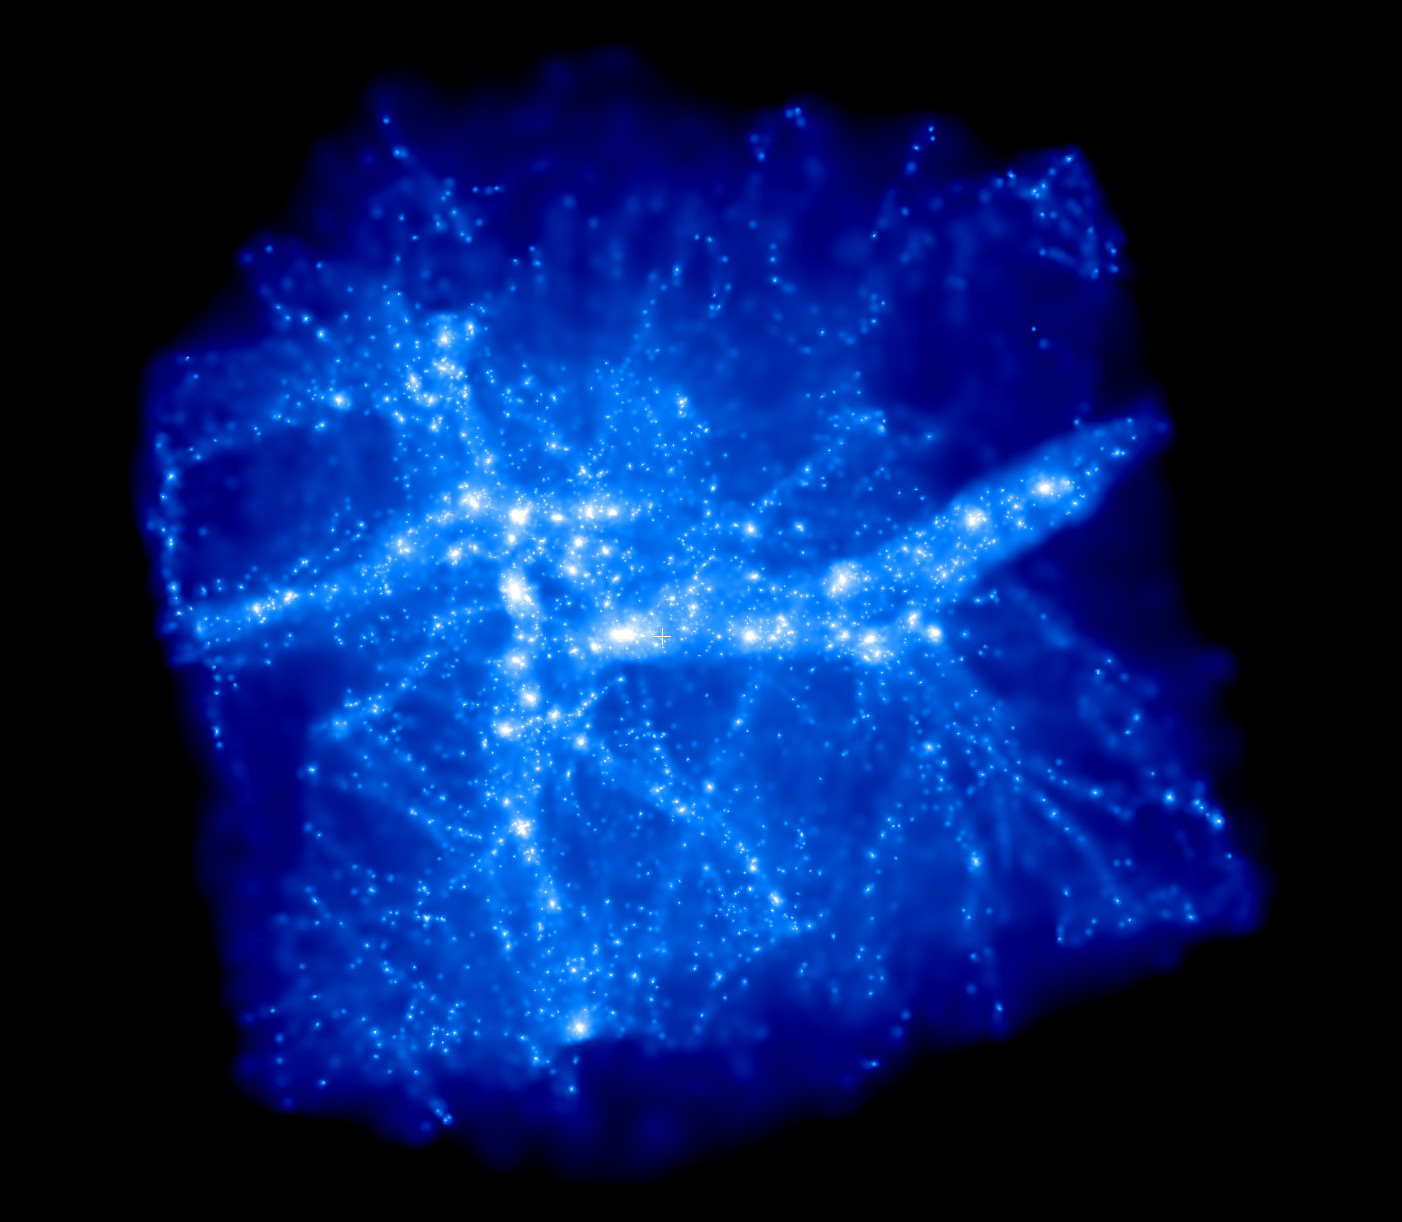
\includegraphics[scale=0.12]{dr5d5_r256/rotate_00188.jpg} 
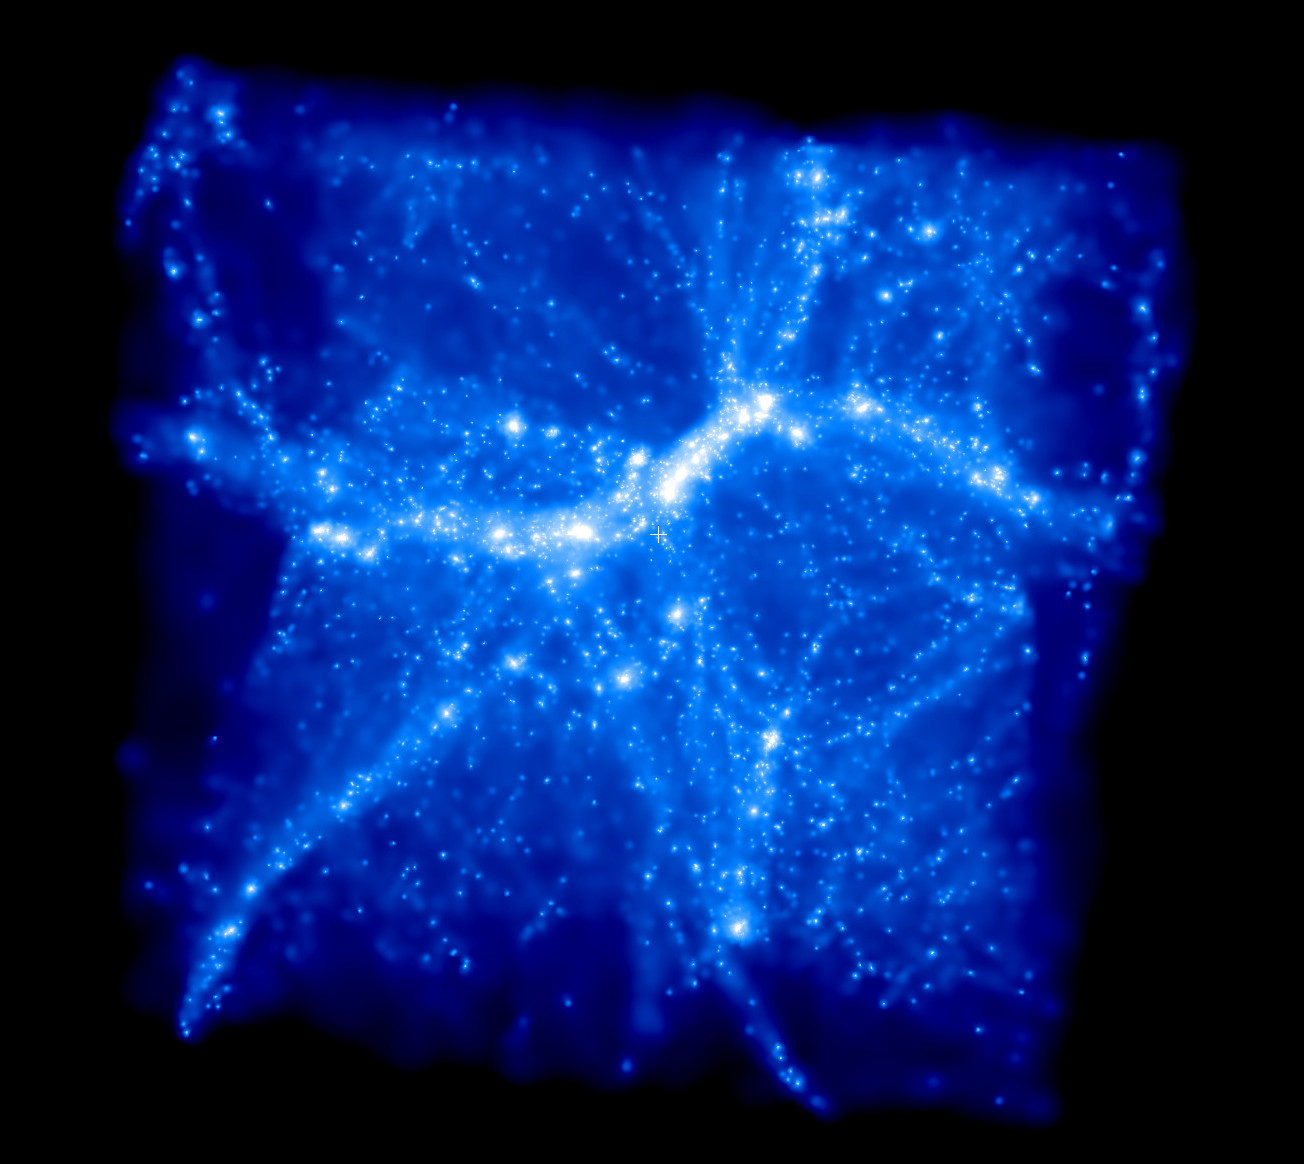
\includegraphics[scale=0.12]{dr5d5_r256/rotate_00320.jpg} \\

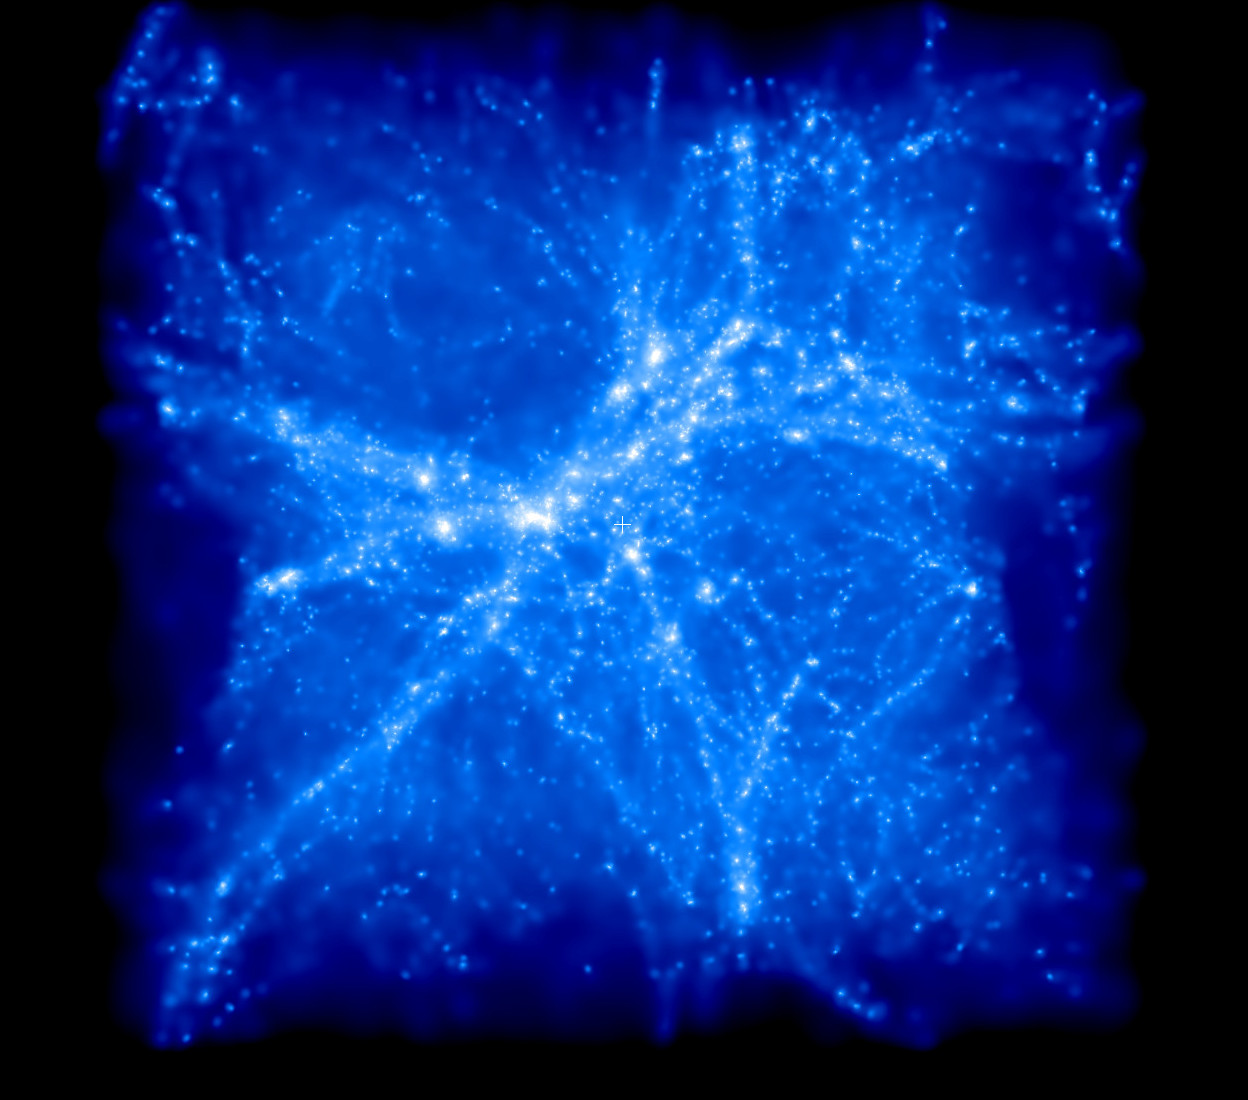
\includegraphics[scale=0.12]{dr5d5_r256/evolve_00160.jpg} 
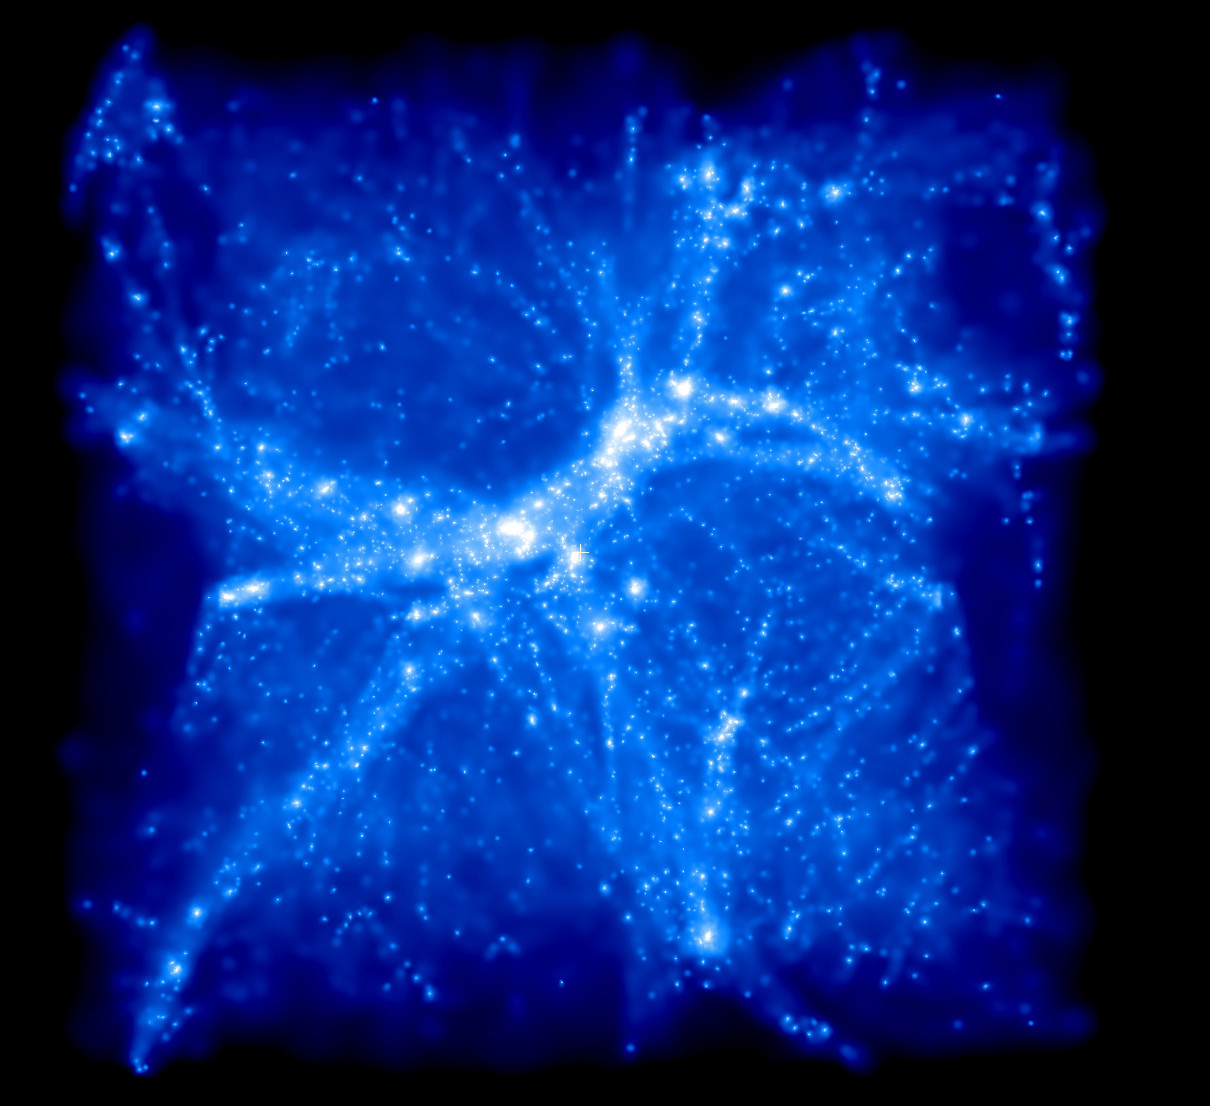
\includegraphics[scale=0.12]{dr5d5_r256/evolve_00304.jpg} 
%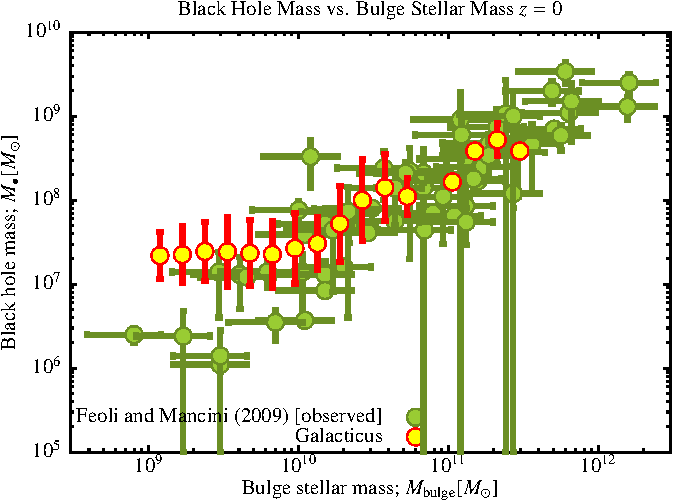
\includegraphics[scale=0.6]{drd5_r256/Black_Hole_vs_Bulge_Mass.pdf}
%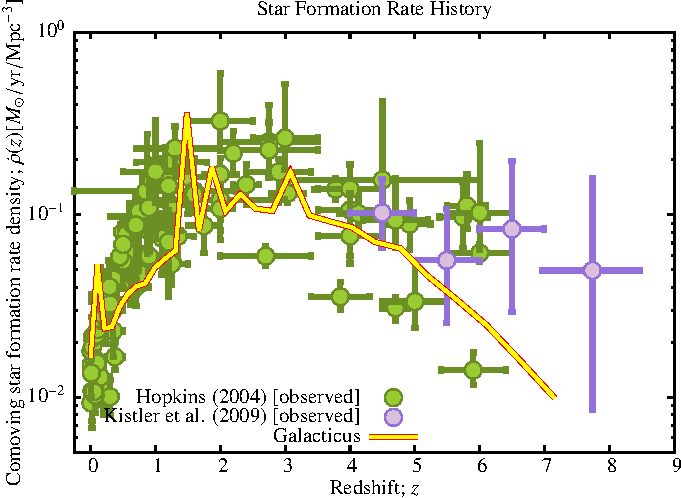
\includegraphics[scale=0.6]{drd5_r256/Star_Formation_History.pdf}
%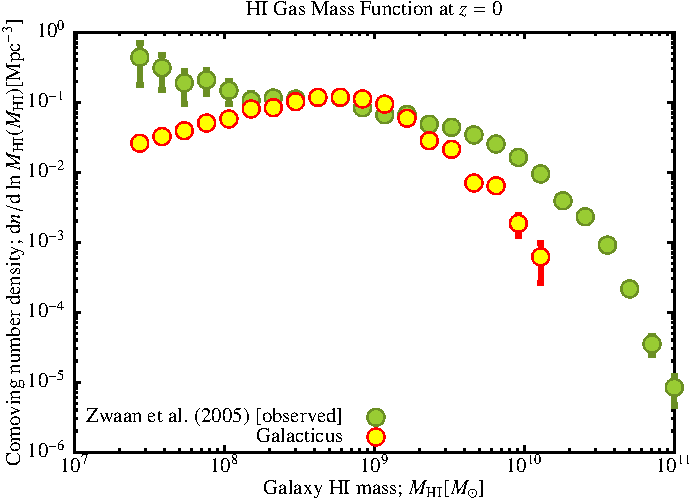
\includegraphics[scale=0.6]{drd5_r256/HI_Gas_Mass_Function.pdf}

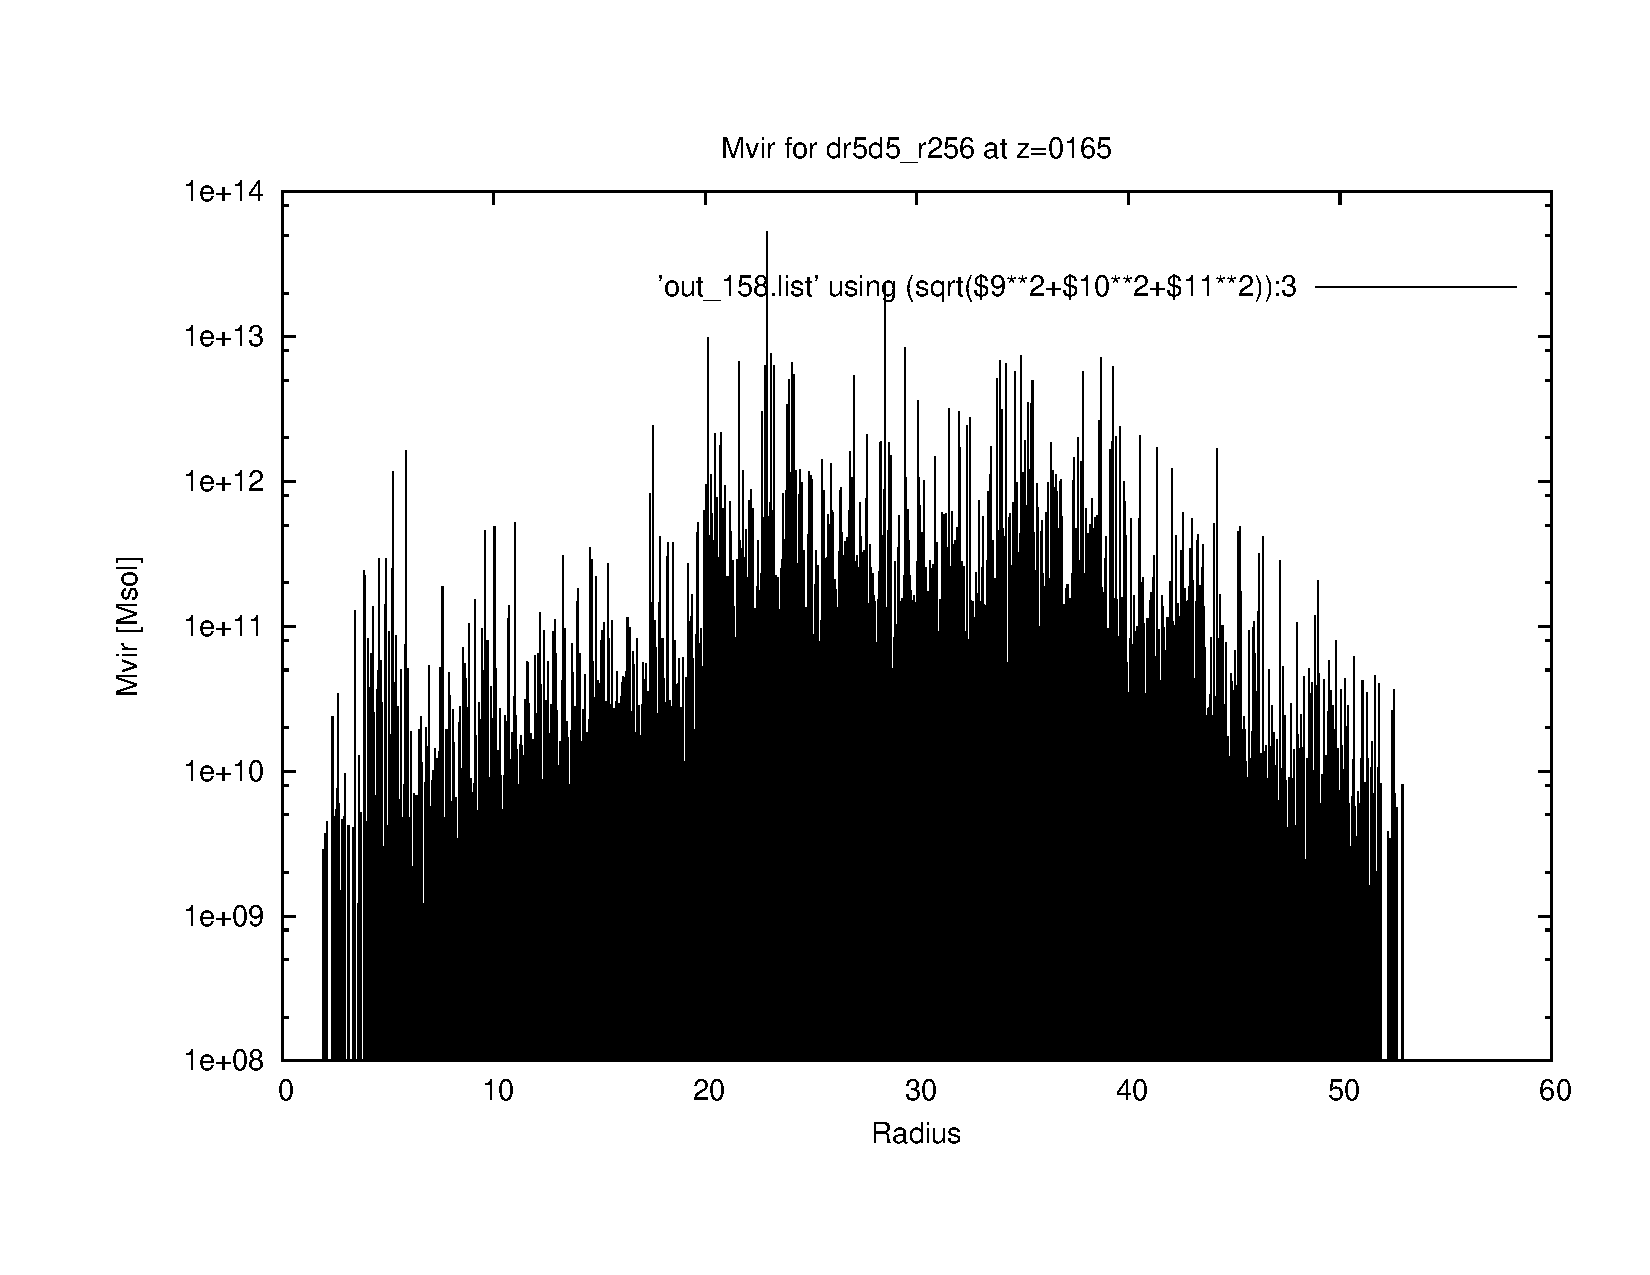
\includegraphics[scale=0.3]{dr5d5_r256/plot_mvir_z0165.pdf}
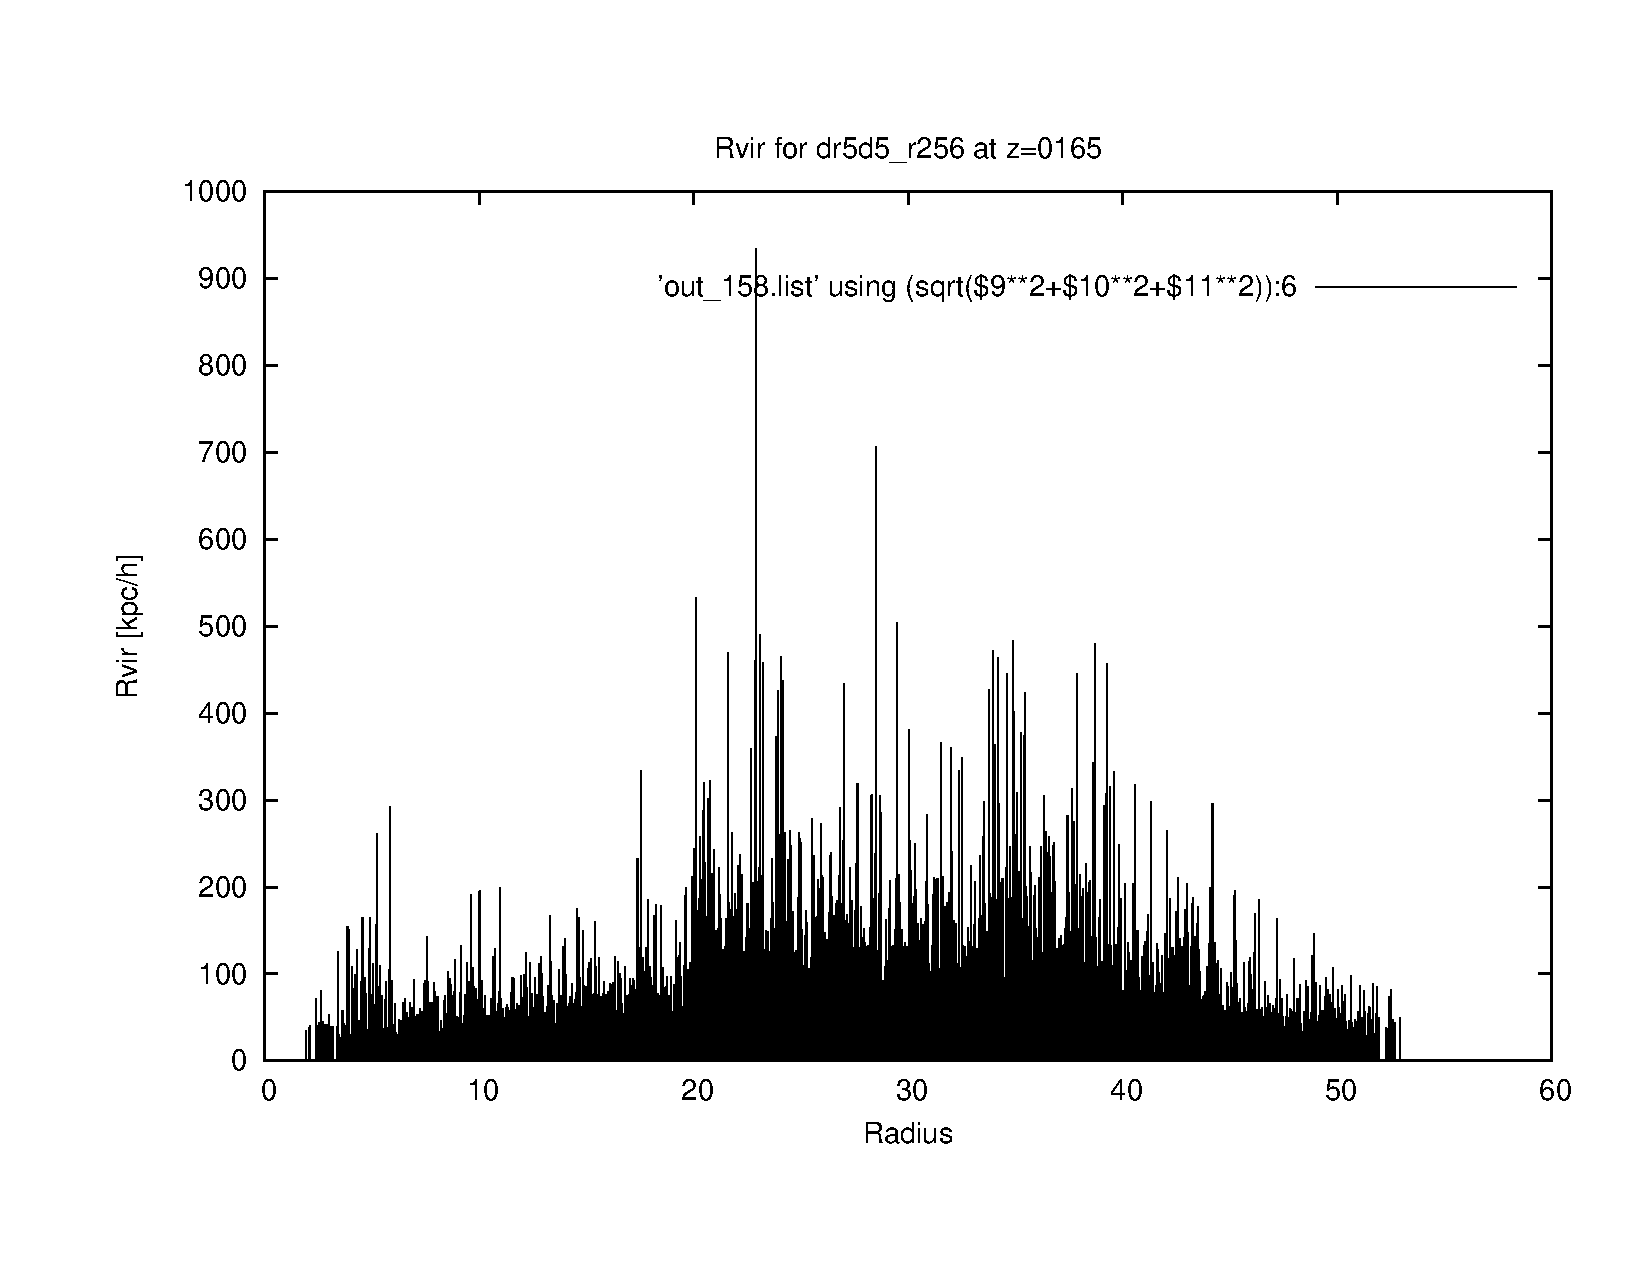
\includegraphics[scale=0.3]{dr5d5_r256/plot_rvir_z0165.pdf}
% 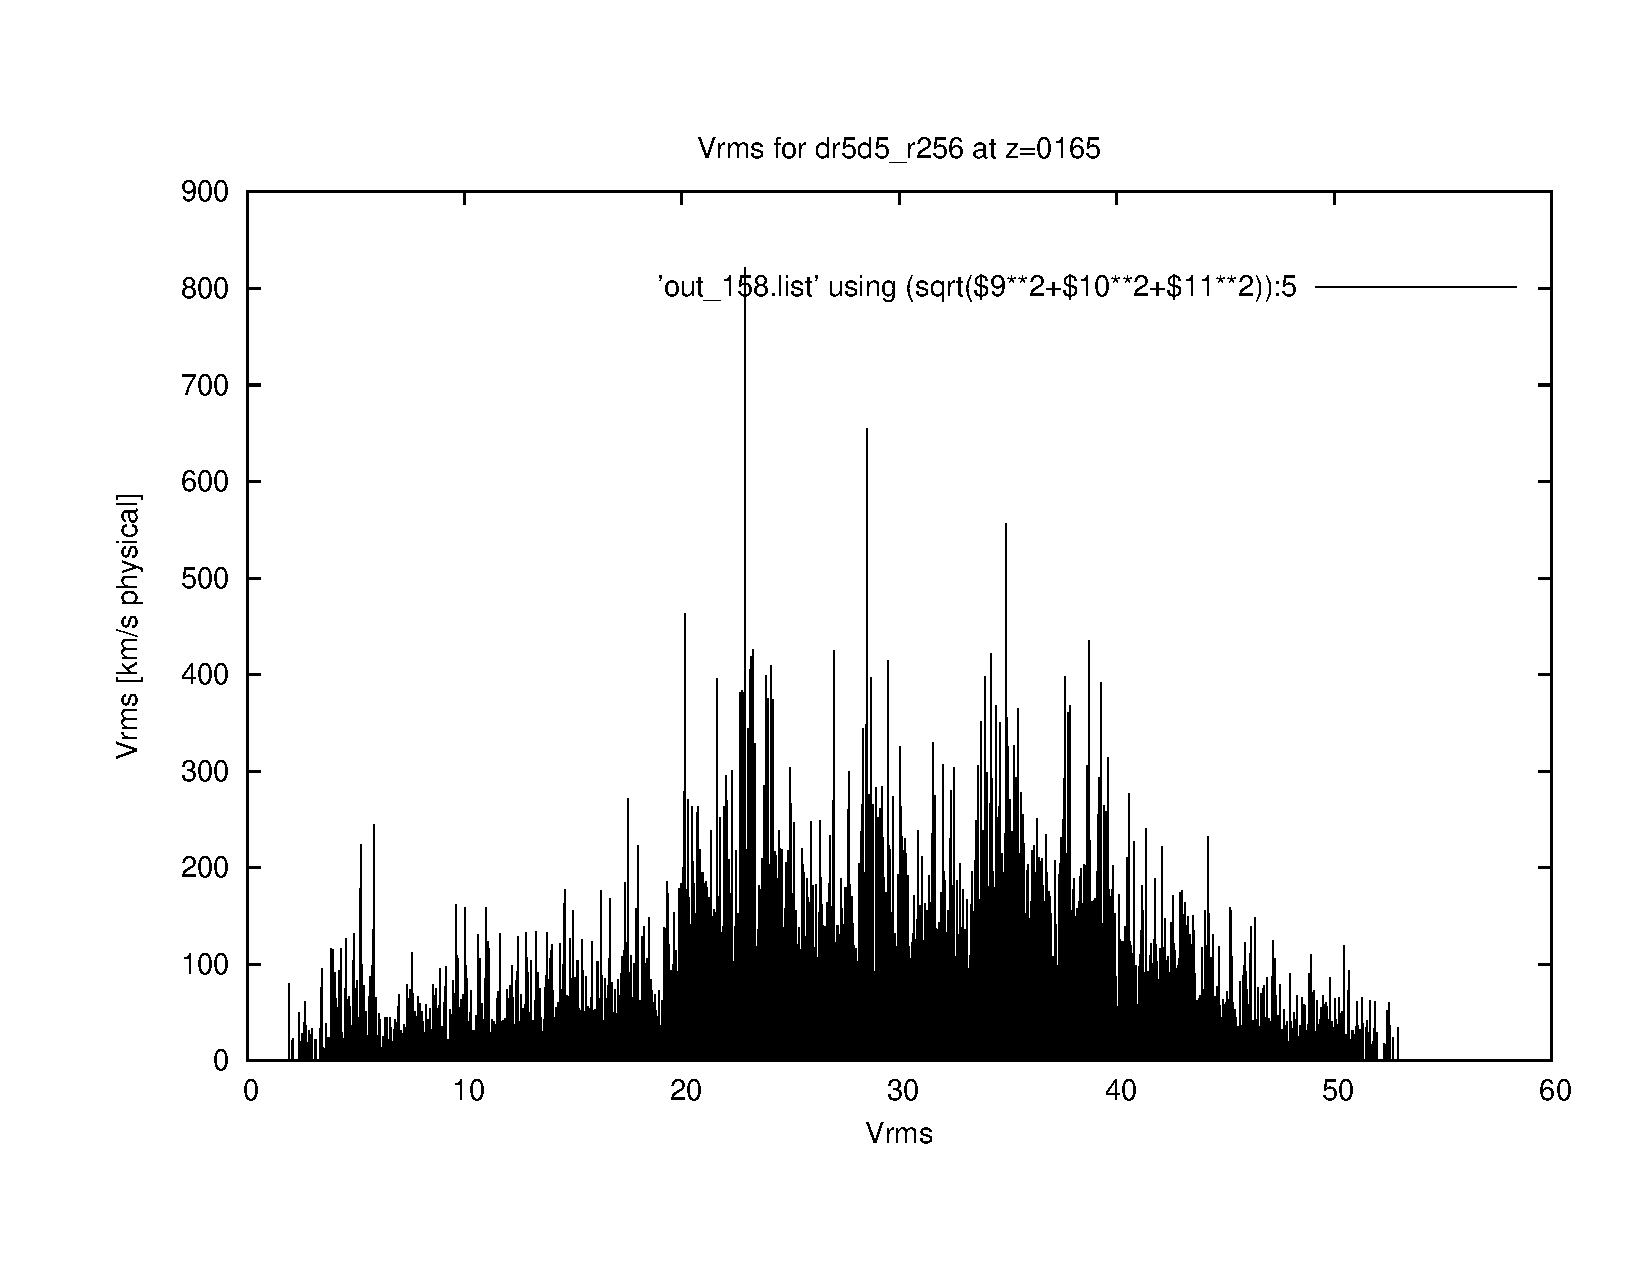
\includegraphics[scale=0.3]{dr5d5_r256/plot_vrms_z0165.pdf} 
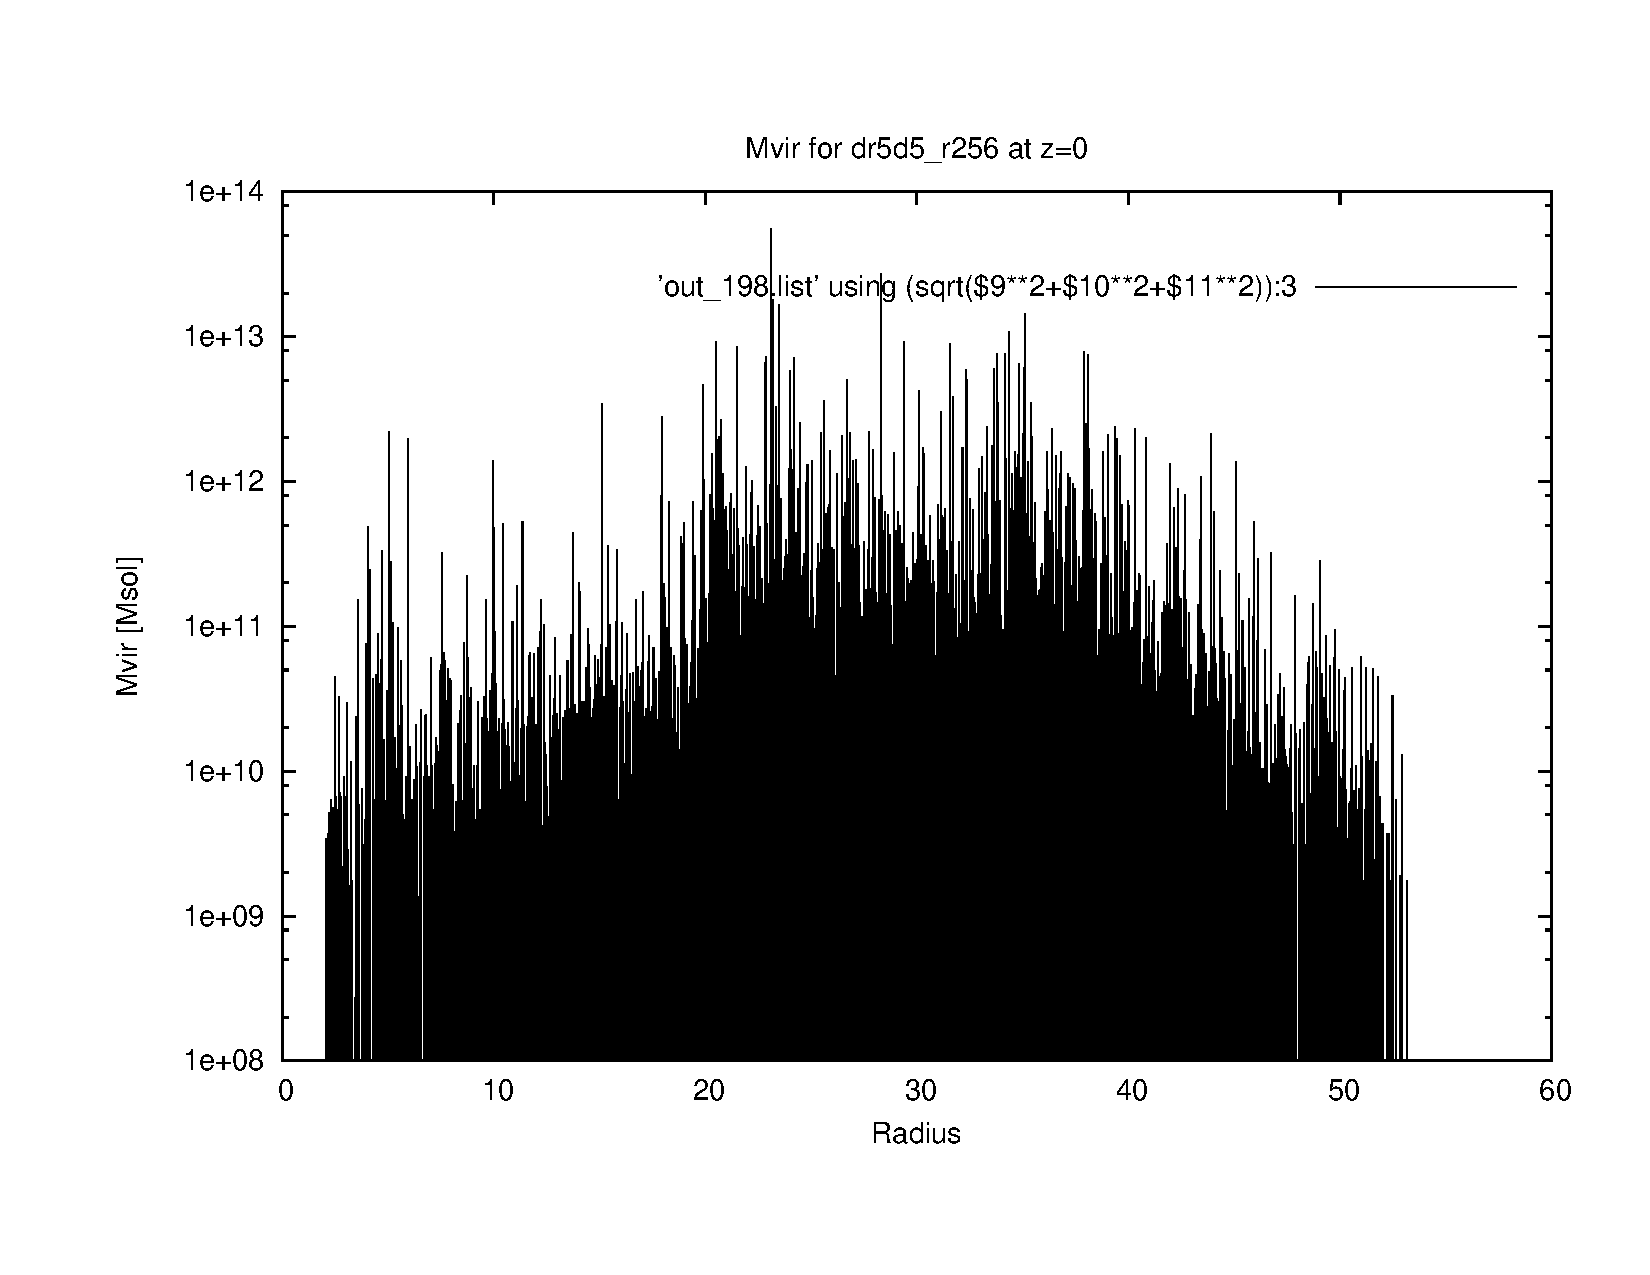
\includegraphics[scale=0.3]{dr5d5_r256/plot_mvir_z0.pdf}
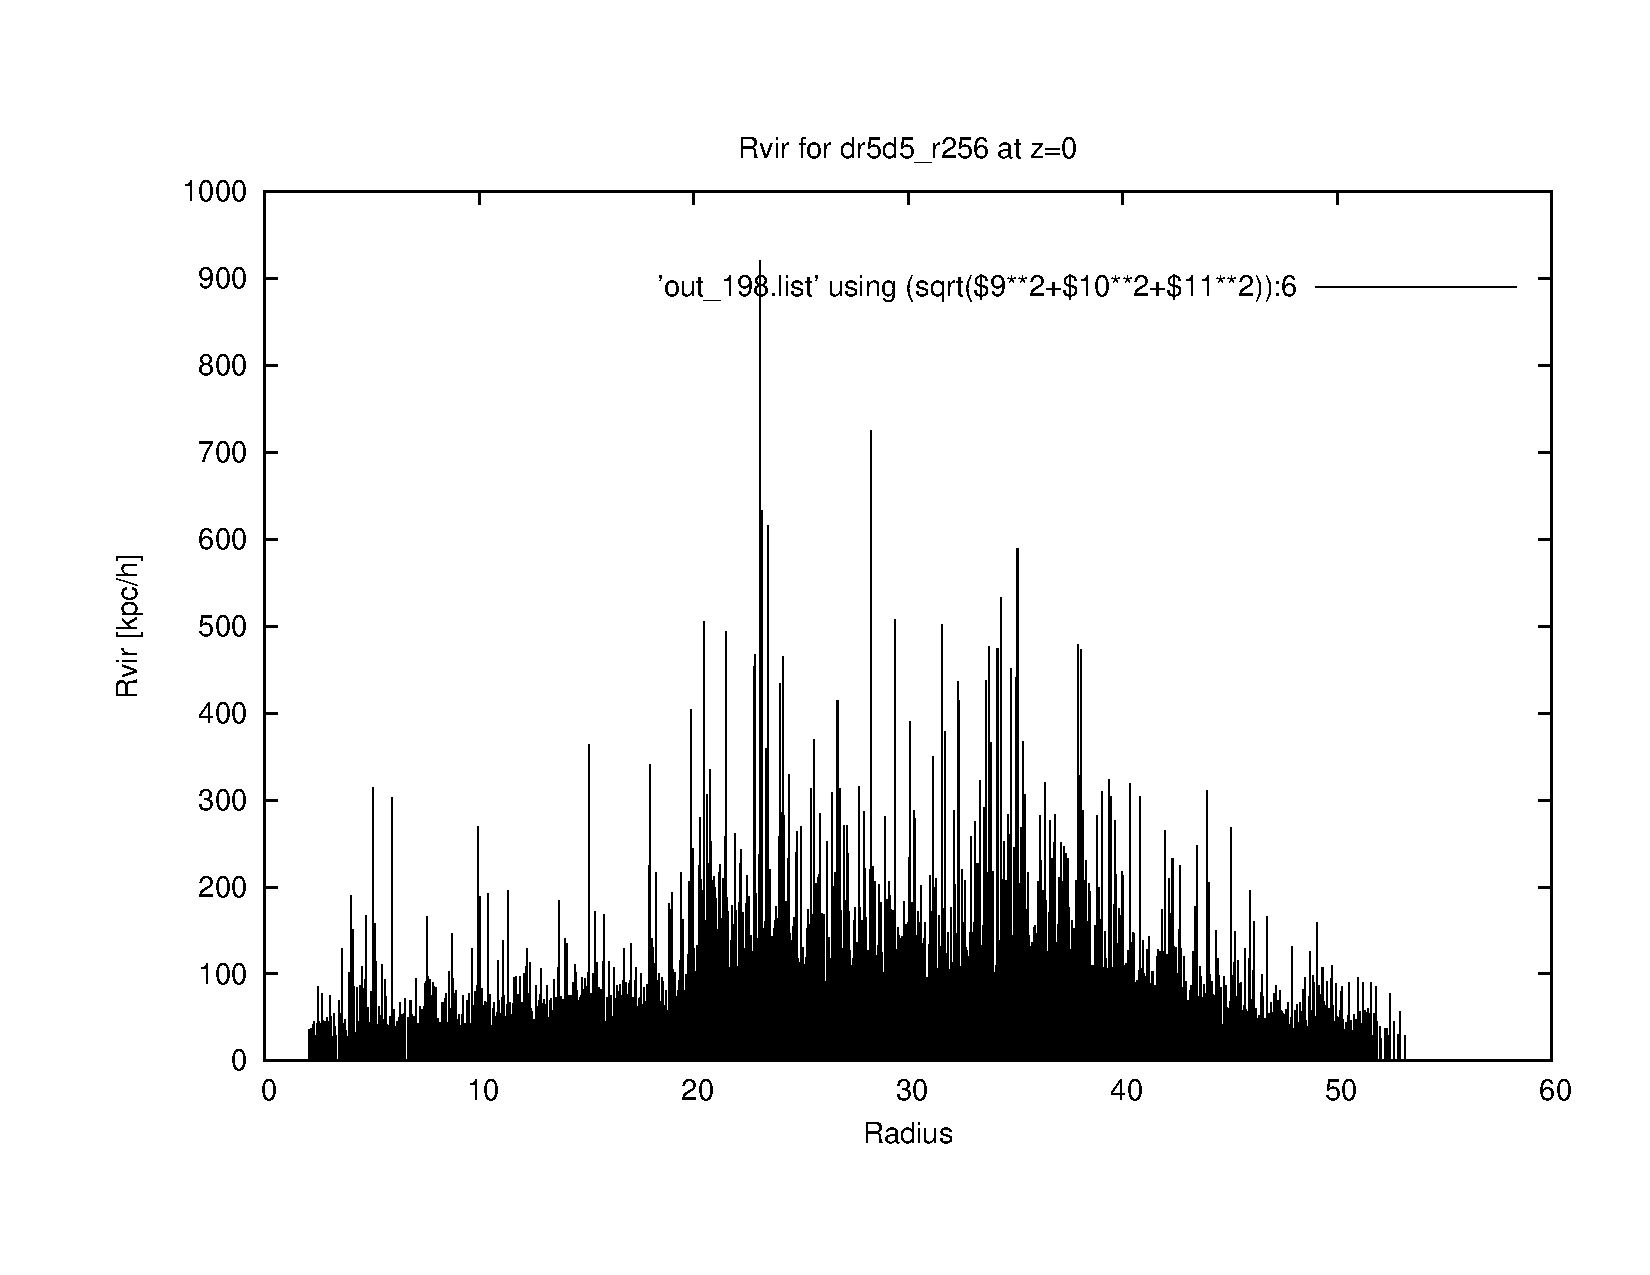
\includegraphics[scale=0.3]{dr5d5_r256/plot_rvir_z0.pdf}
% 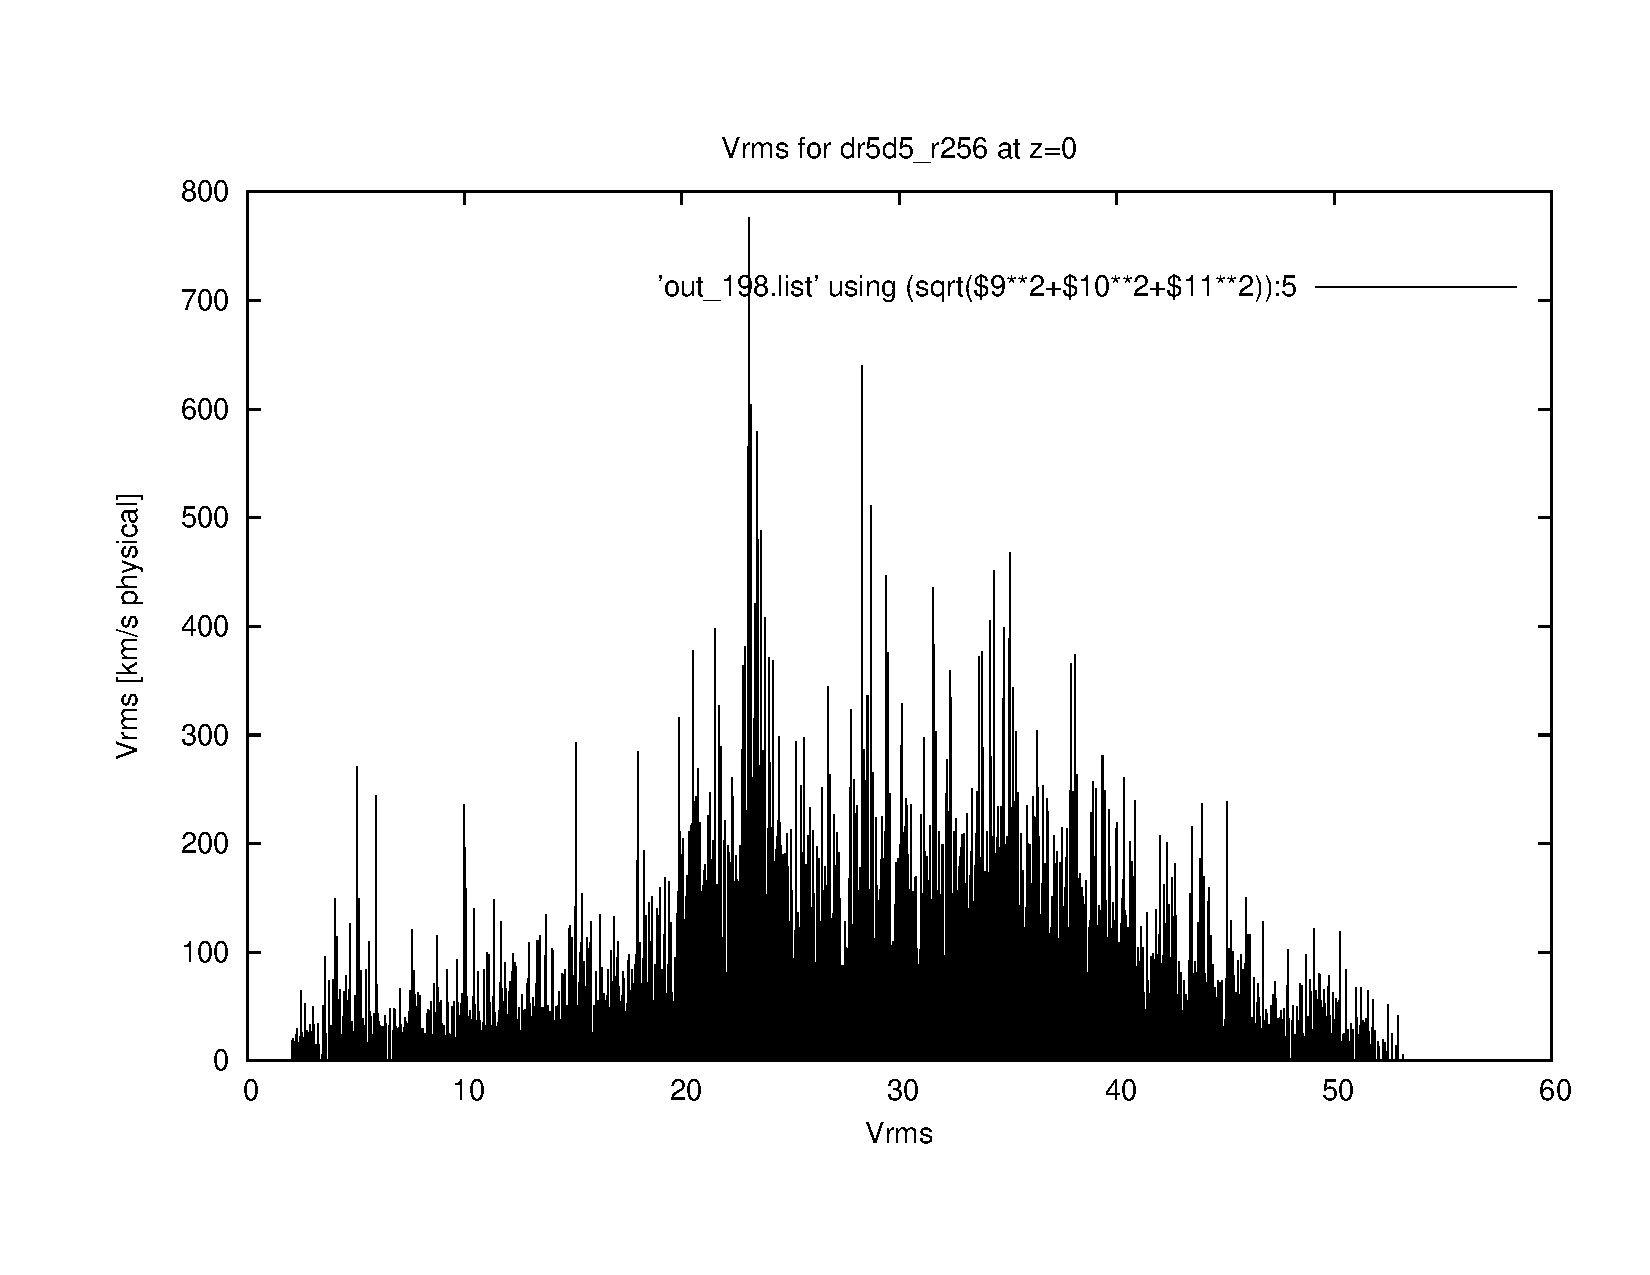
\includegraphics[scale=0.3]{dr5d5_r256/plot_vrms_z0.pdf}

is being galacticussed \\
\textsc{consistenttreed} $\surd$ \\
\textsc{rockstarred} $\surd$ \\
$\rightarrow$  re-rockstar on AMD ...-03 \\
\begin{verbatim}
find_parents_and_cleanup.c:130: 
lookup_new_id: Assertion `new_id' failed.
\end{verbatim}
is being consistenttreed \\ 

% 
%
%
%
%
%
%
%

\newpage

\subsection{drd5\_r256 ($\sim$)} 

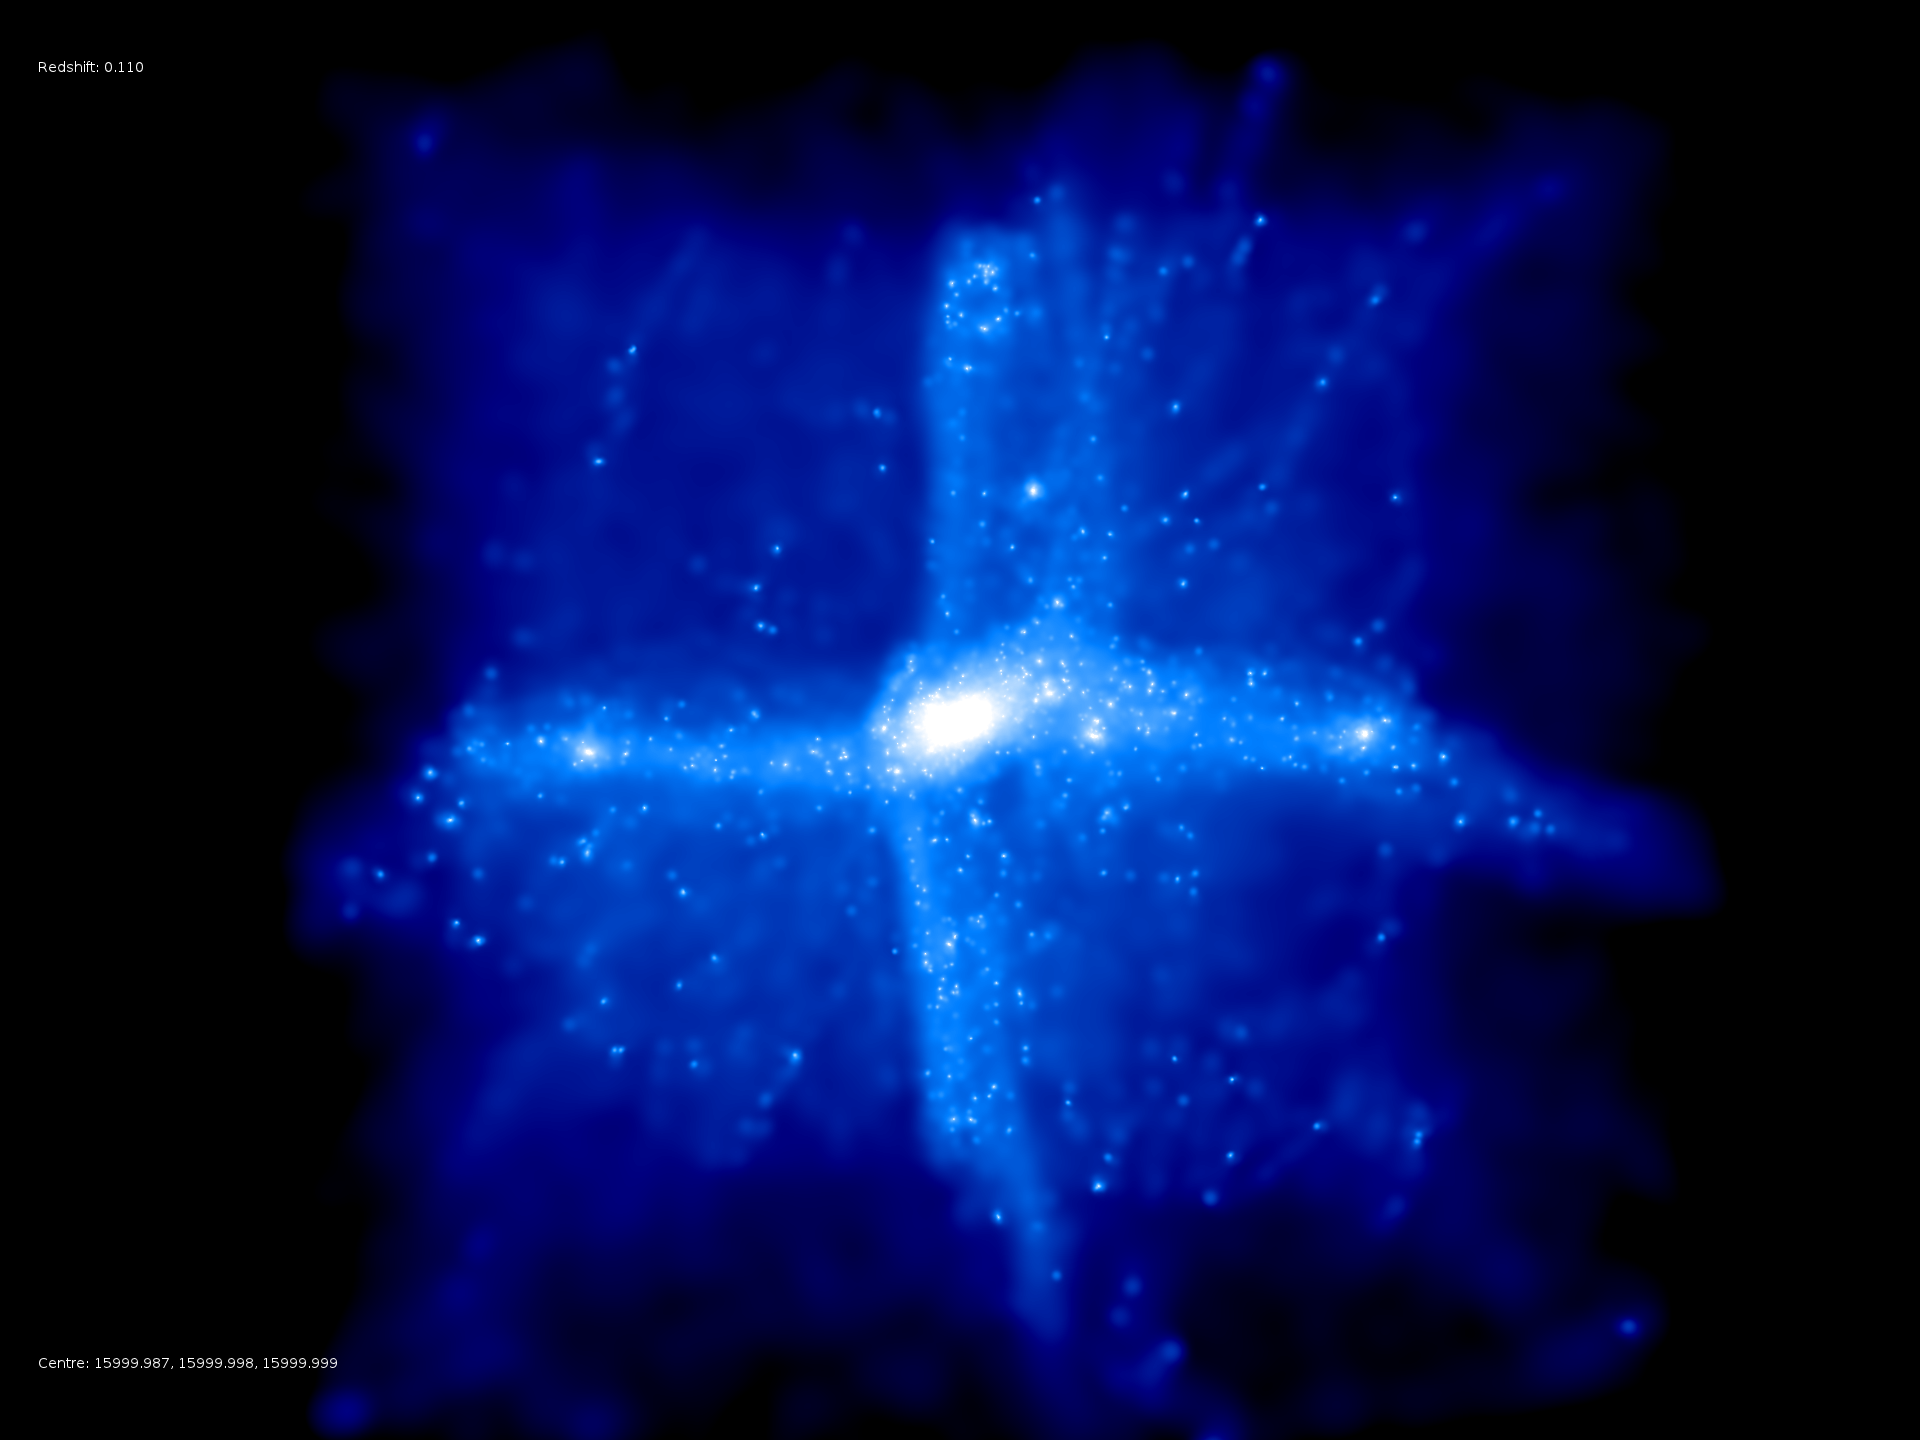
\includegraphics[scale=0.12]{drd5_r256/rotate_1.png} 
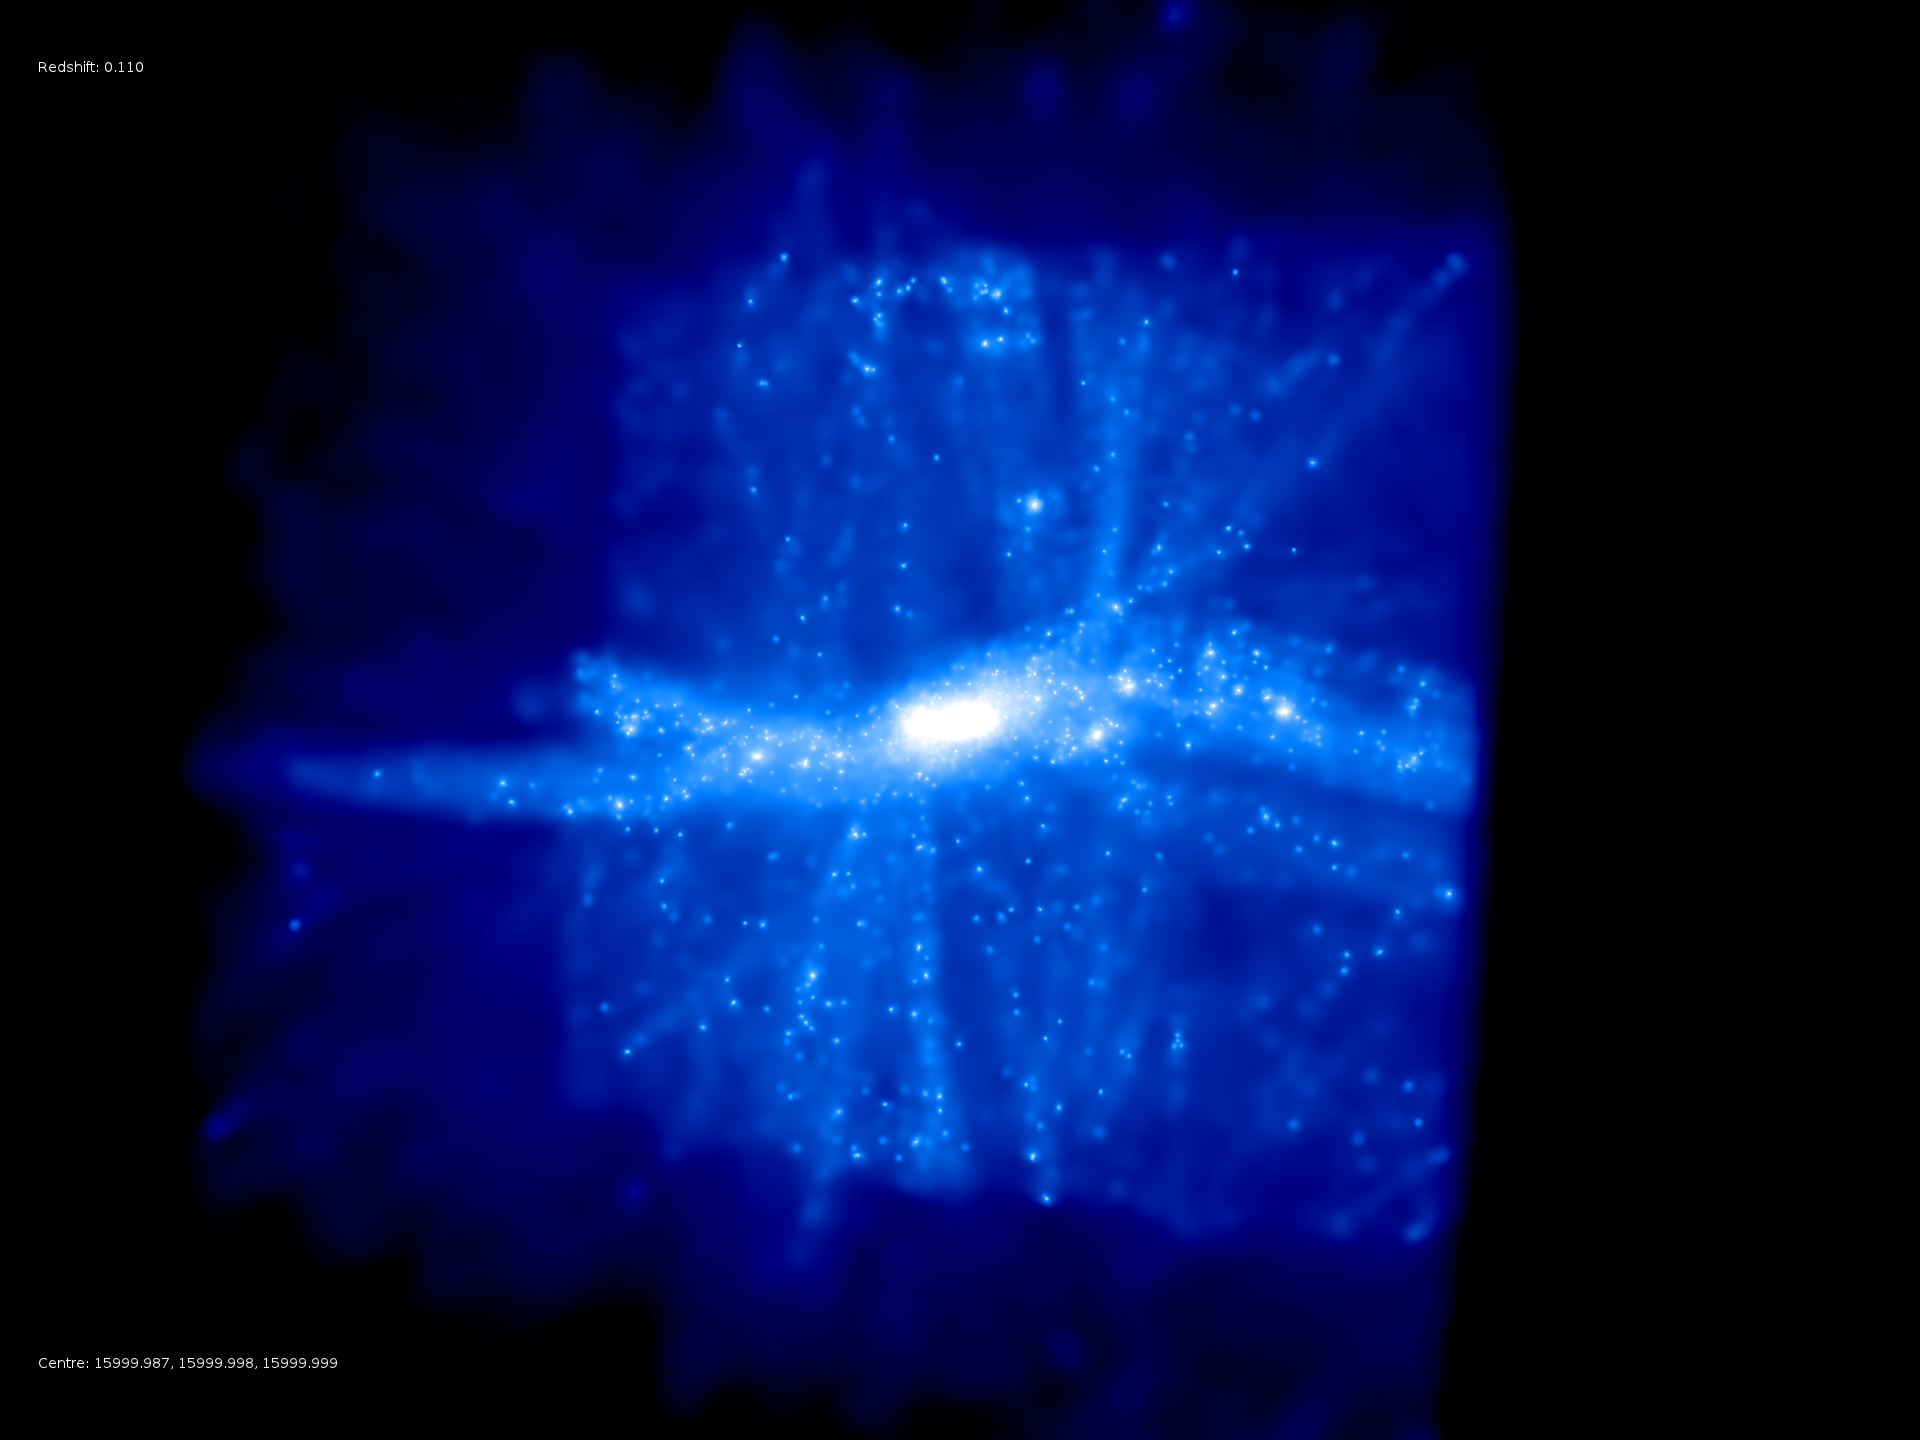
\includegraphics[scale=0.12]{drd5_r256/rotate_2.png} 
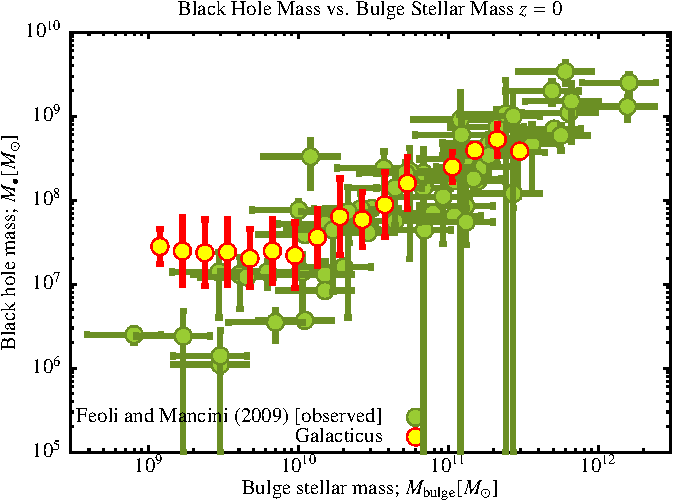
\includegraphics[scale=0.6]{drd5_r256/Plot_Black_Hole_vs_Bulge_Mass.pdf}
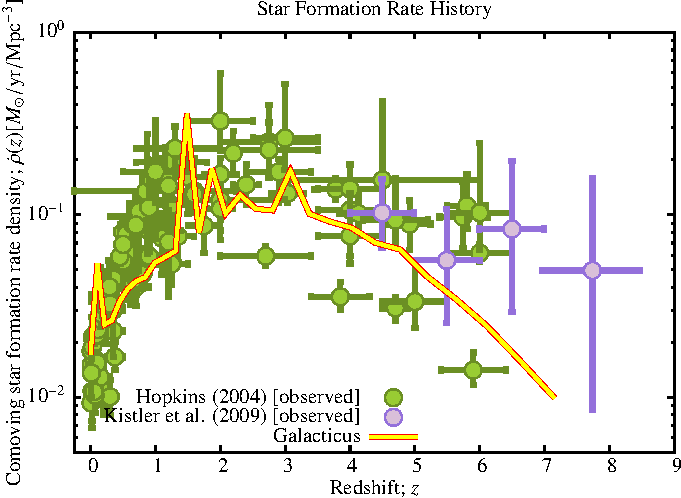
\includegraphics[scale=0.6]{drd5_r256/Plot_Star_Formation_History.pdf}
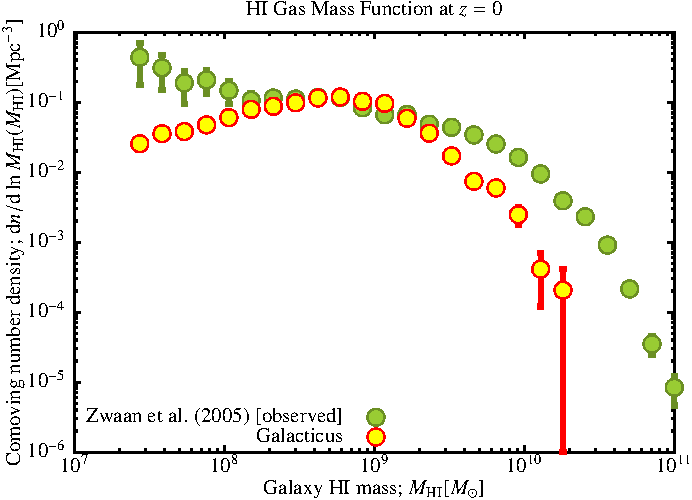
\includegraphics[scale=0.6]{drd5_r256/Plot_HI_Mass_Function.pdf}

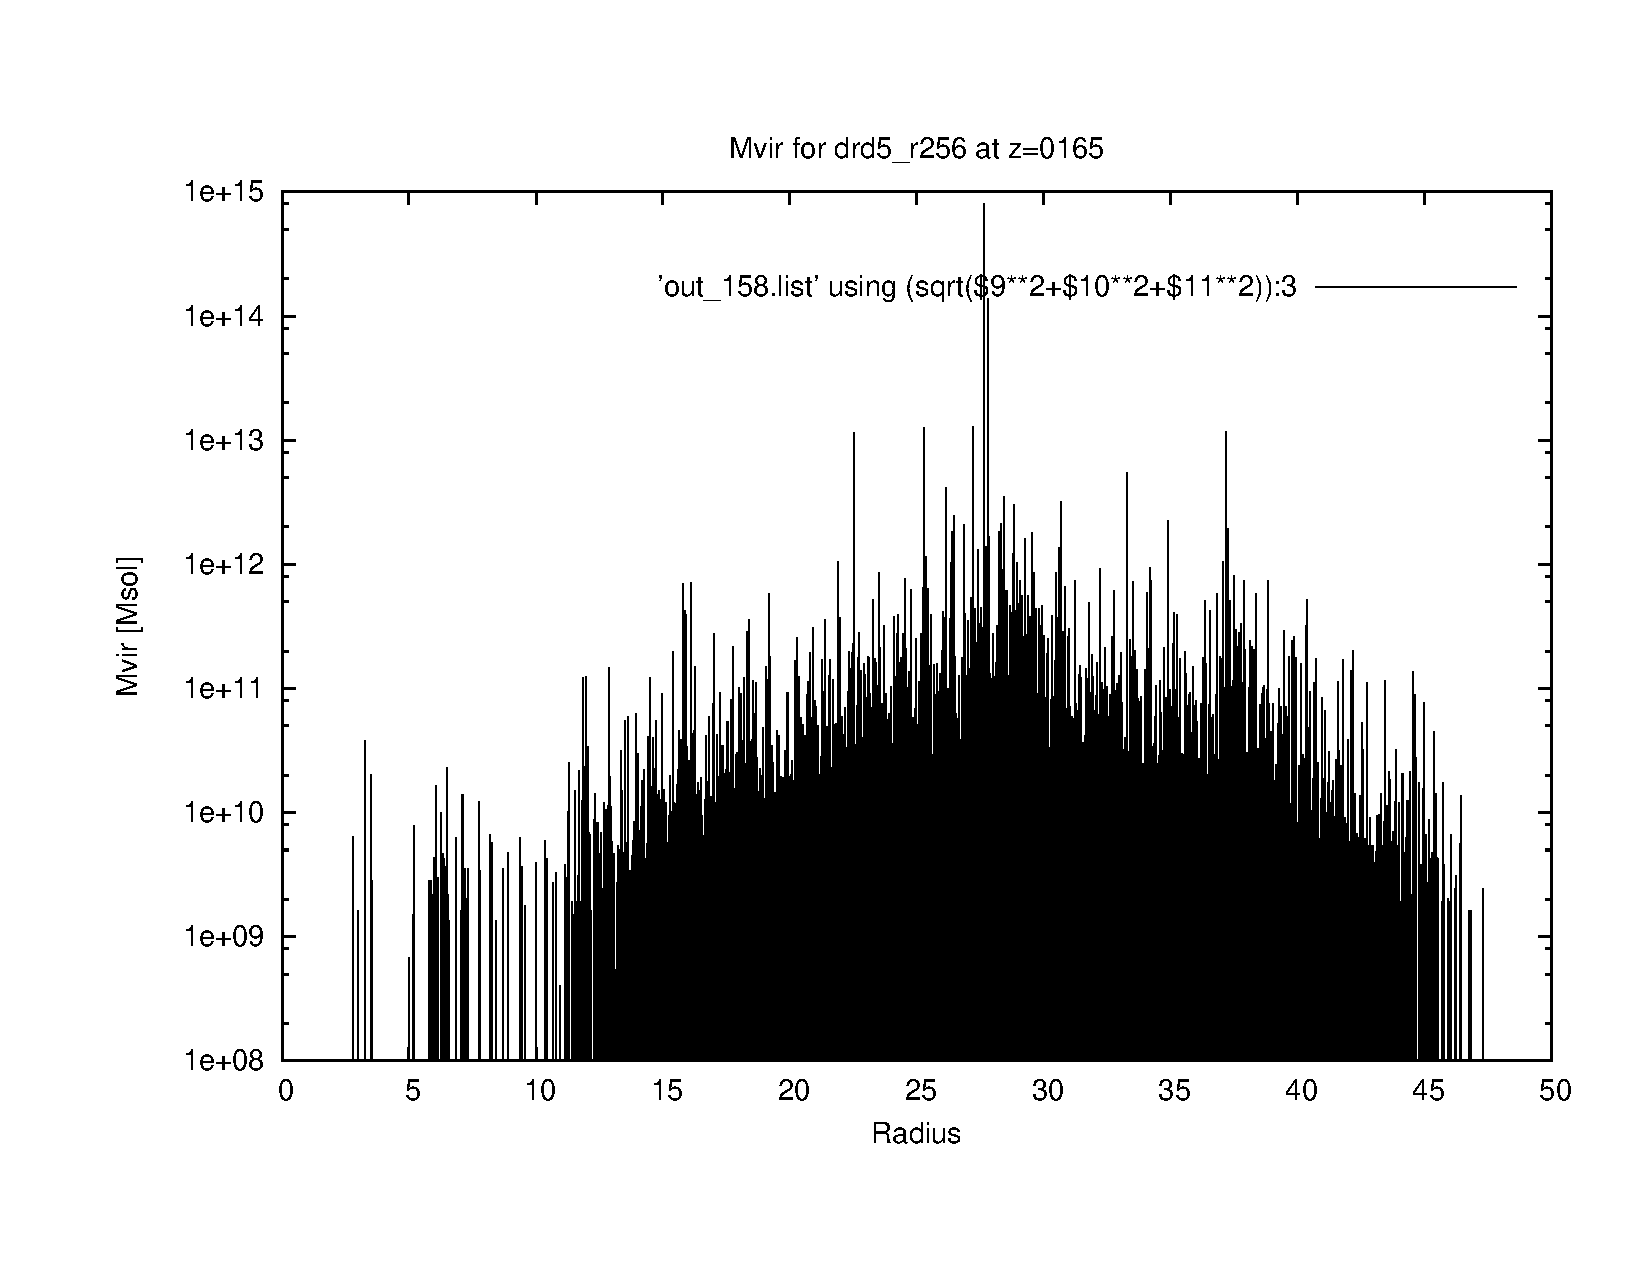
\includegraphics[scale=0.3]{drd5_r256/plot_mvir_z0165.pdf}
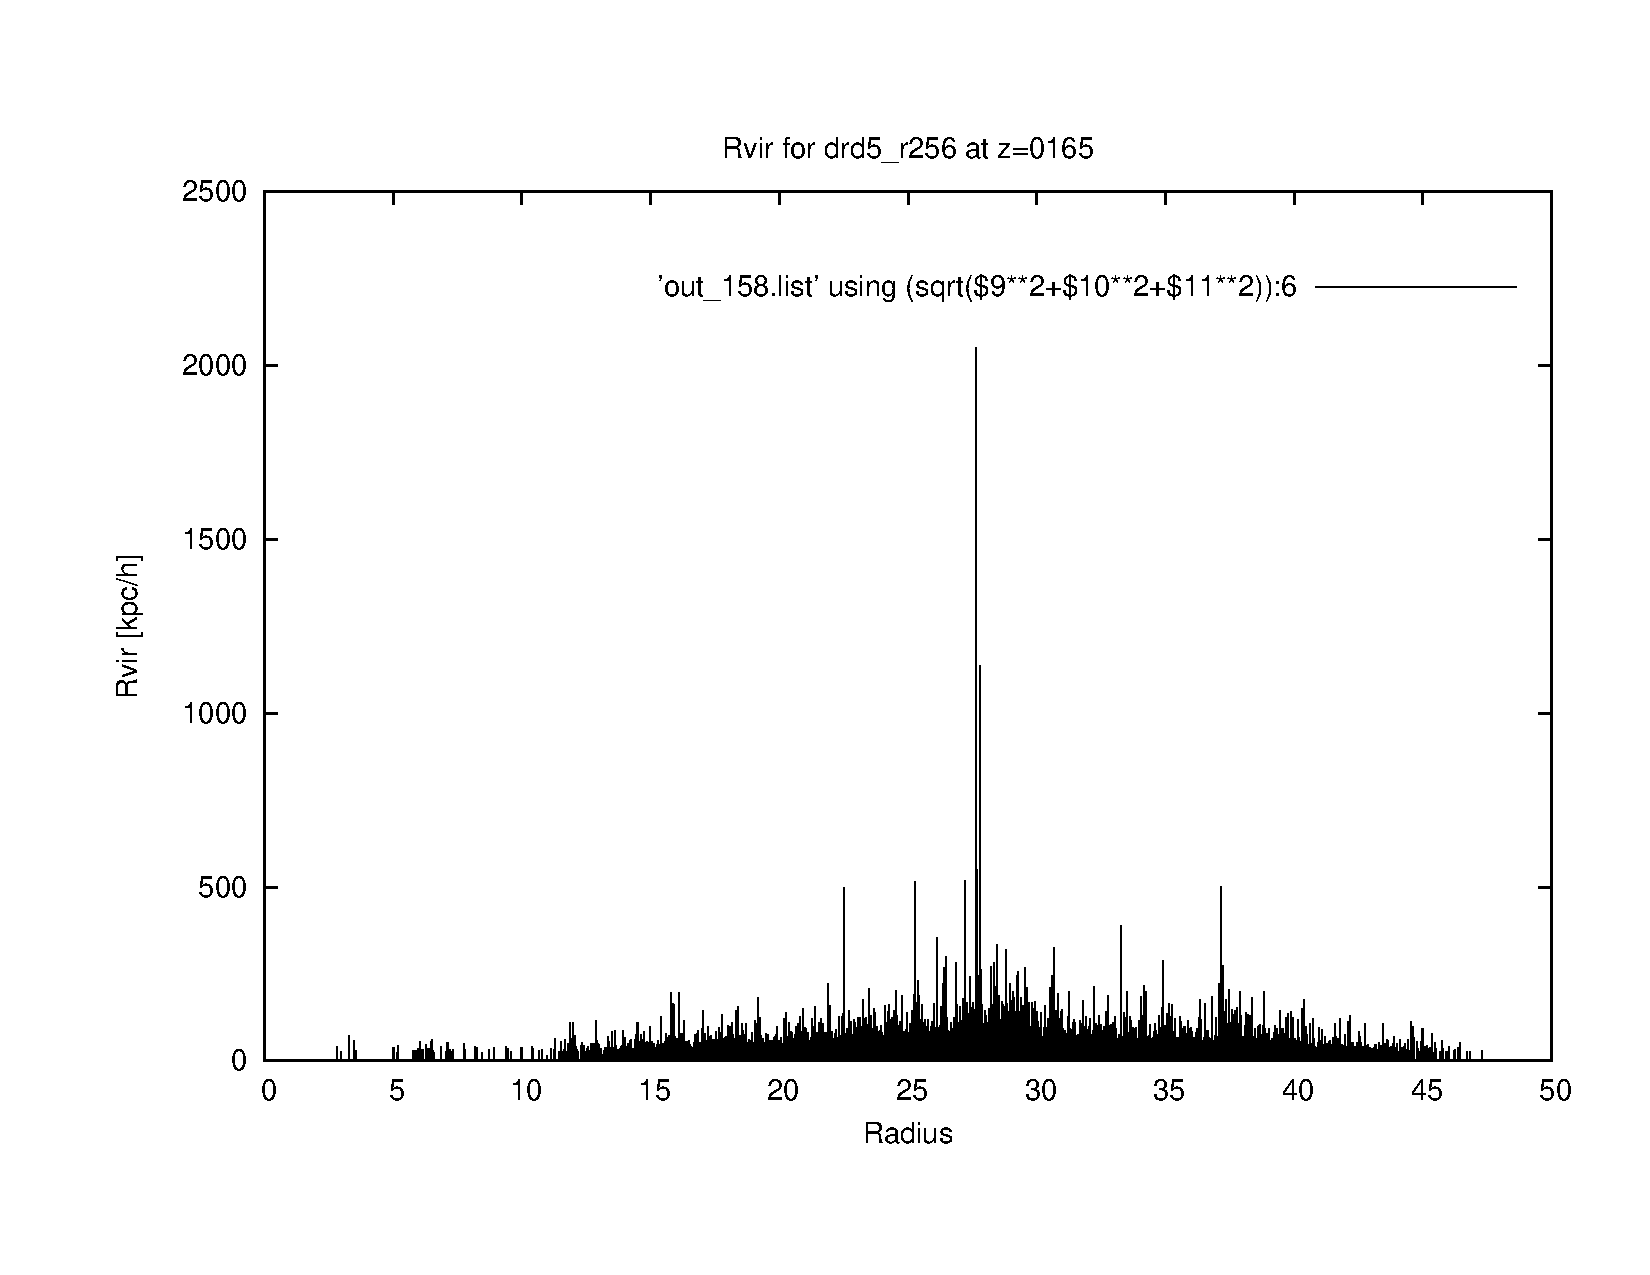
\includegraphics[scale=0.3]{drd5_r256/plot_rvir_z0165.pdf}
% 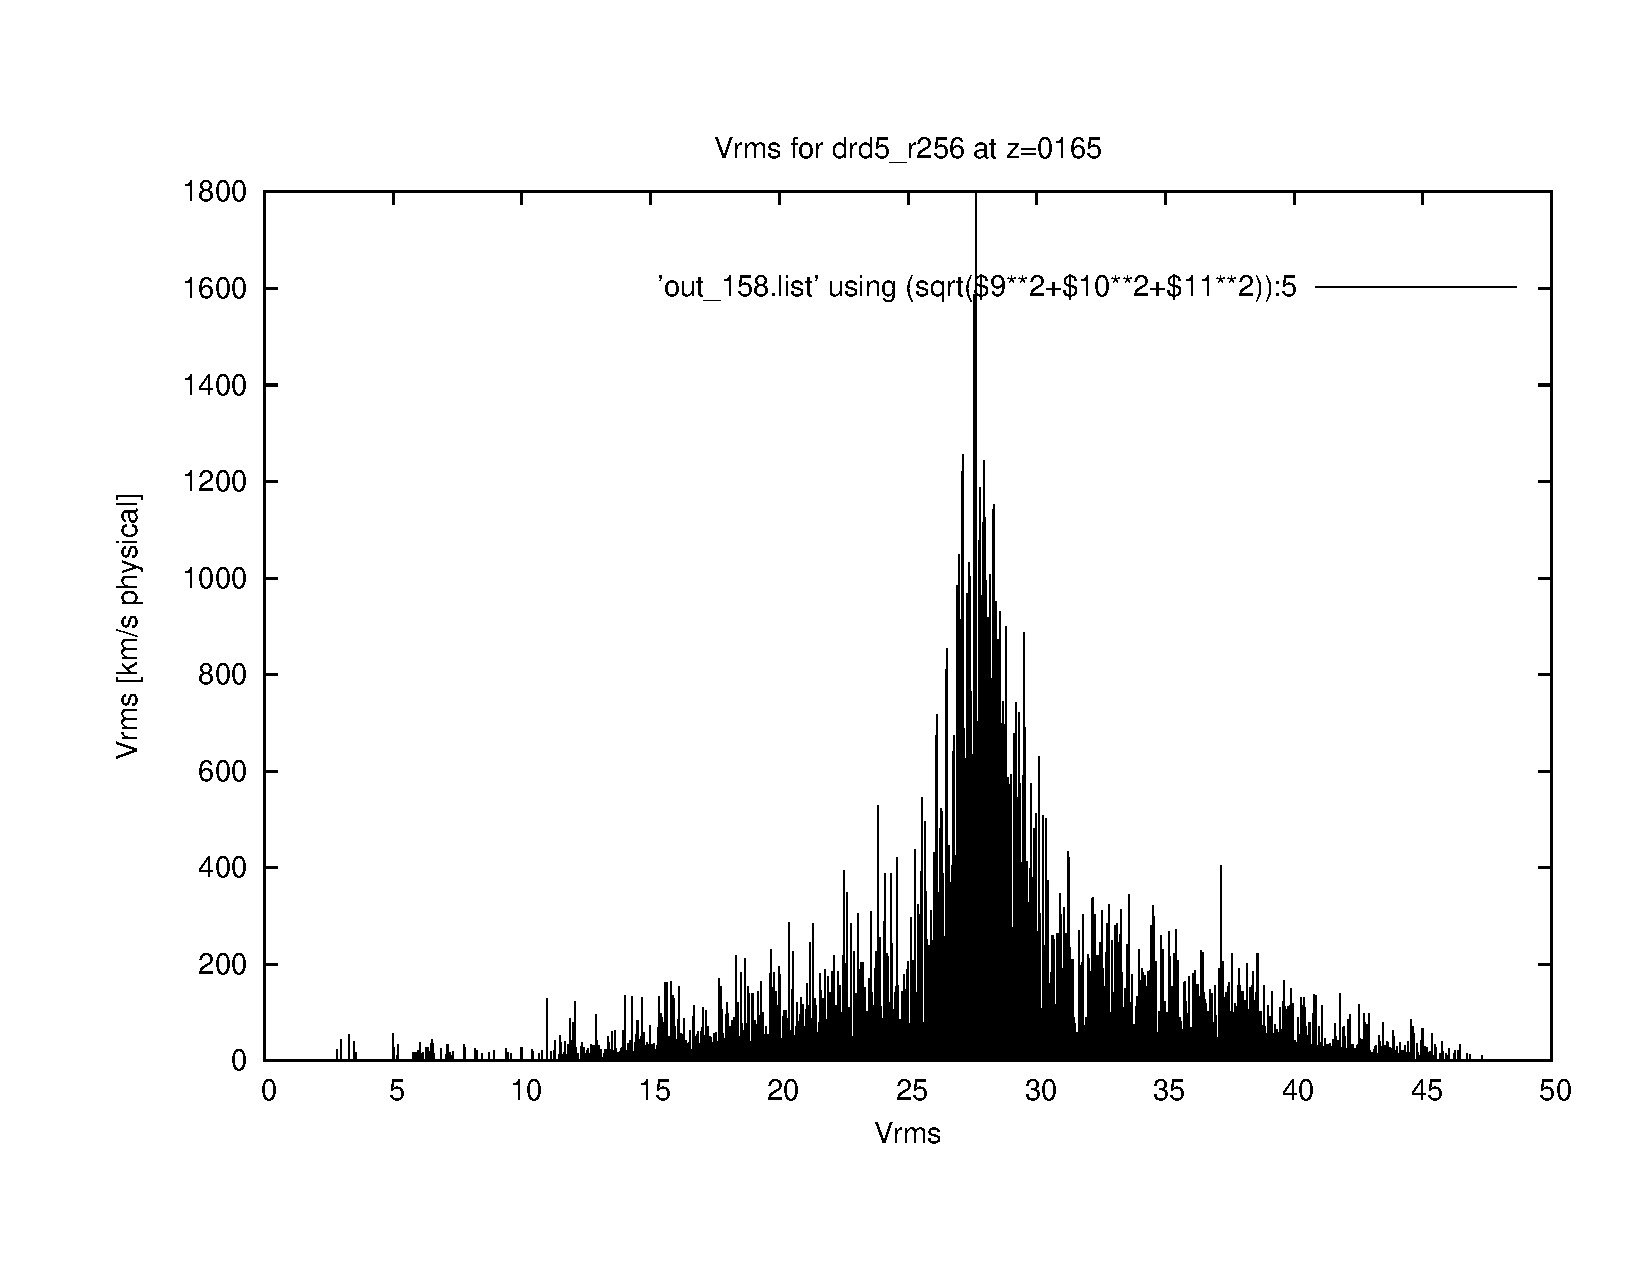
\includegraphics[scale=0.3]{drd5_r256/plot_vrms_z0165.pdf} 
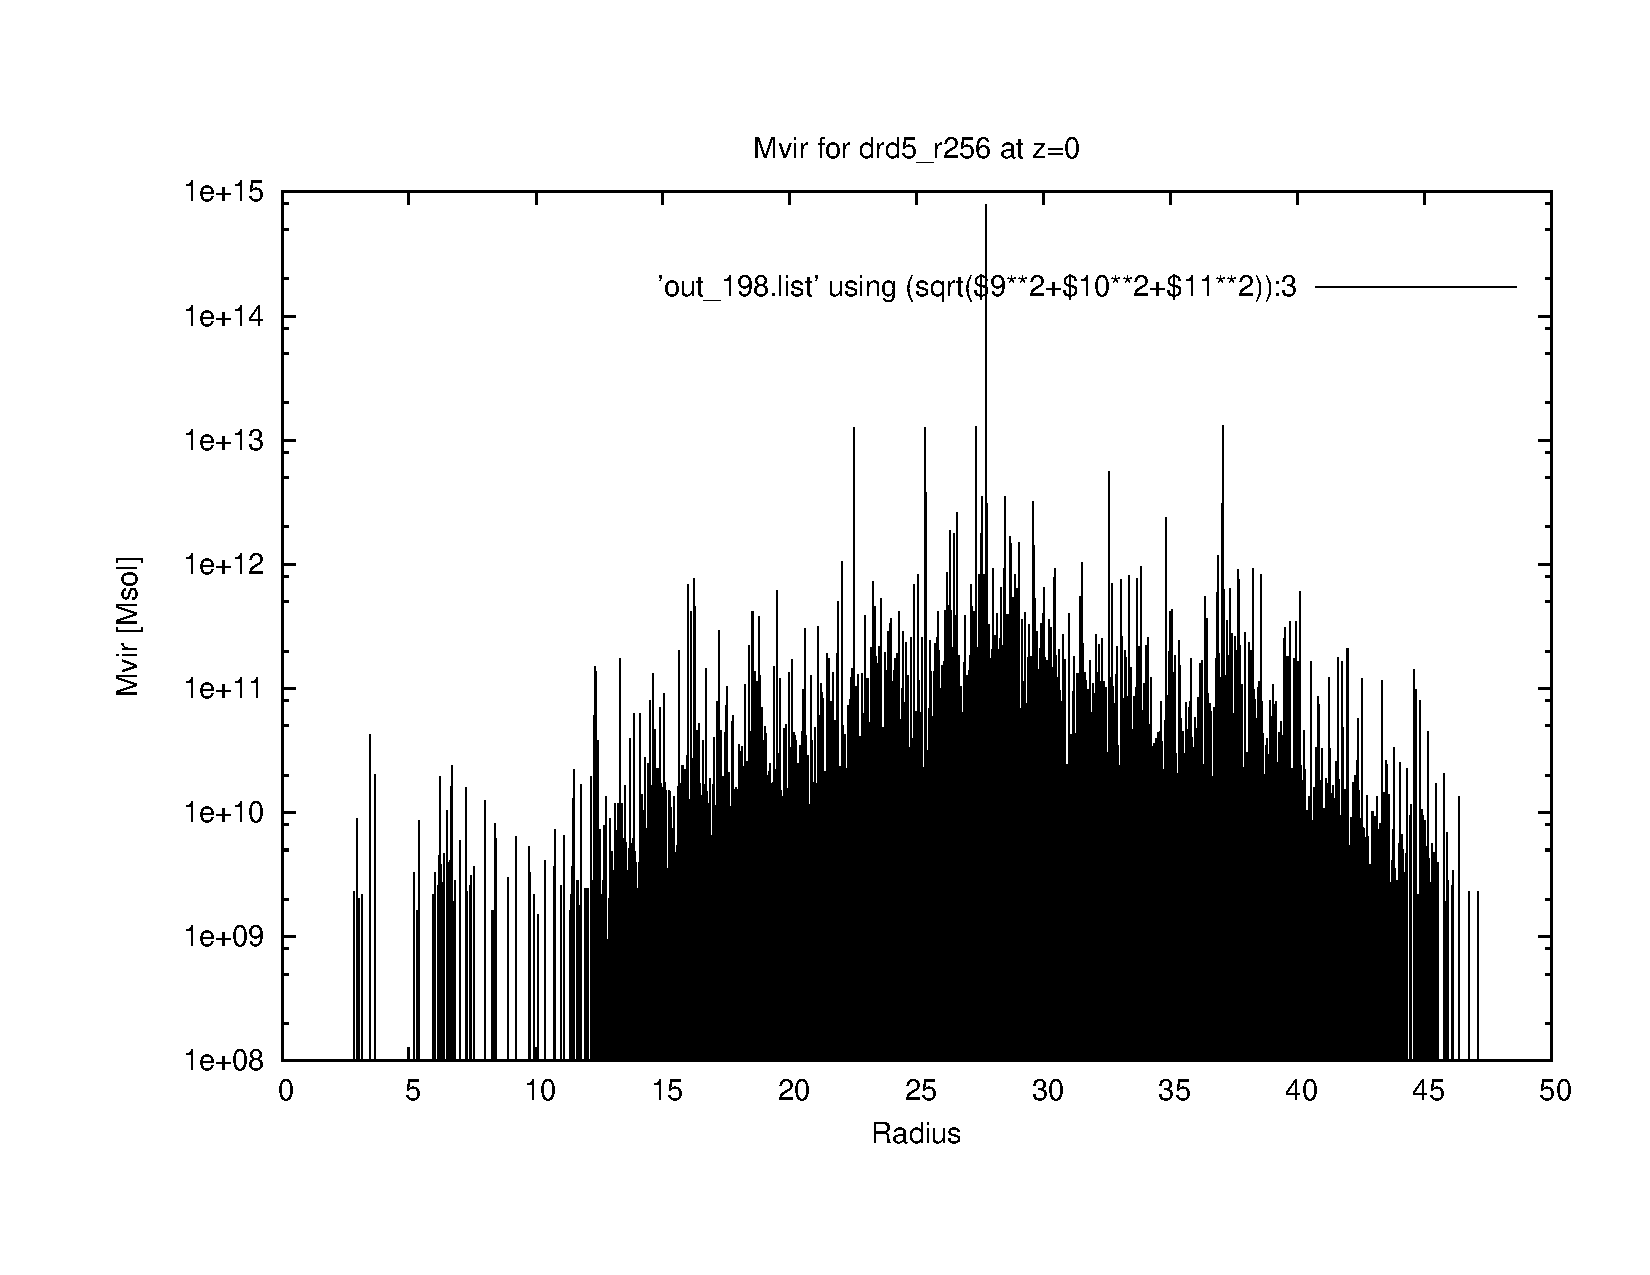
\includegraphics[scale=0.3]{drd5_r256/plot_mvir_z0.pdf}
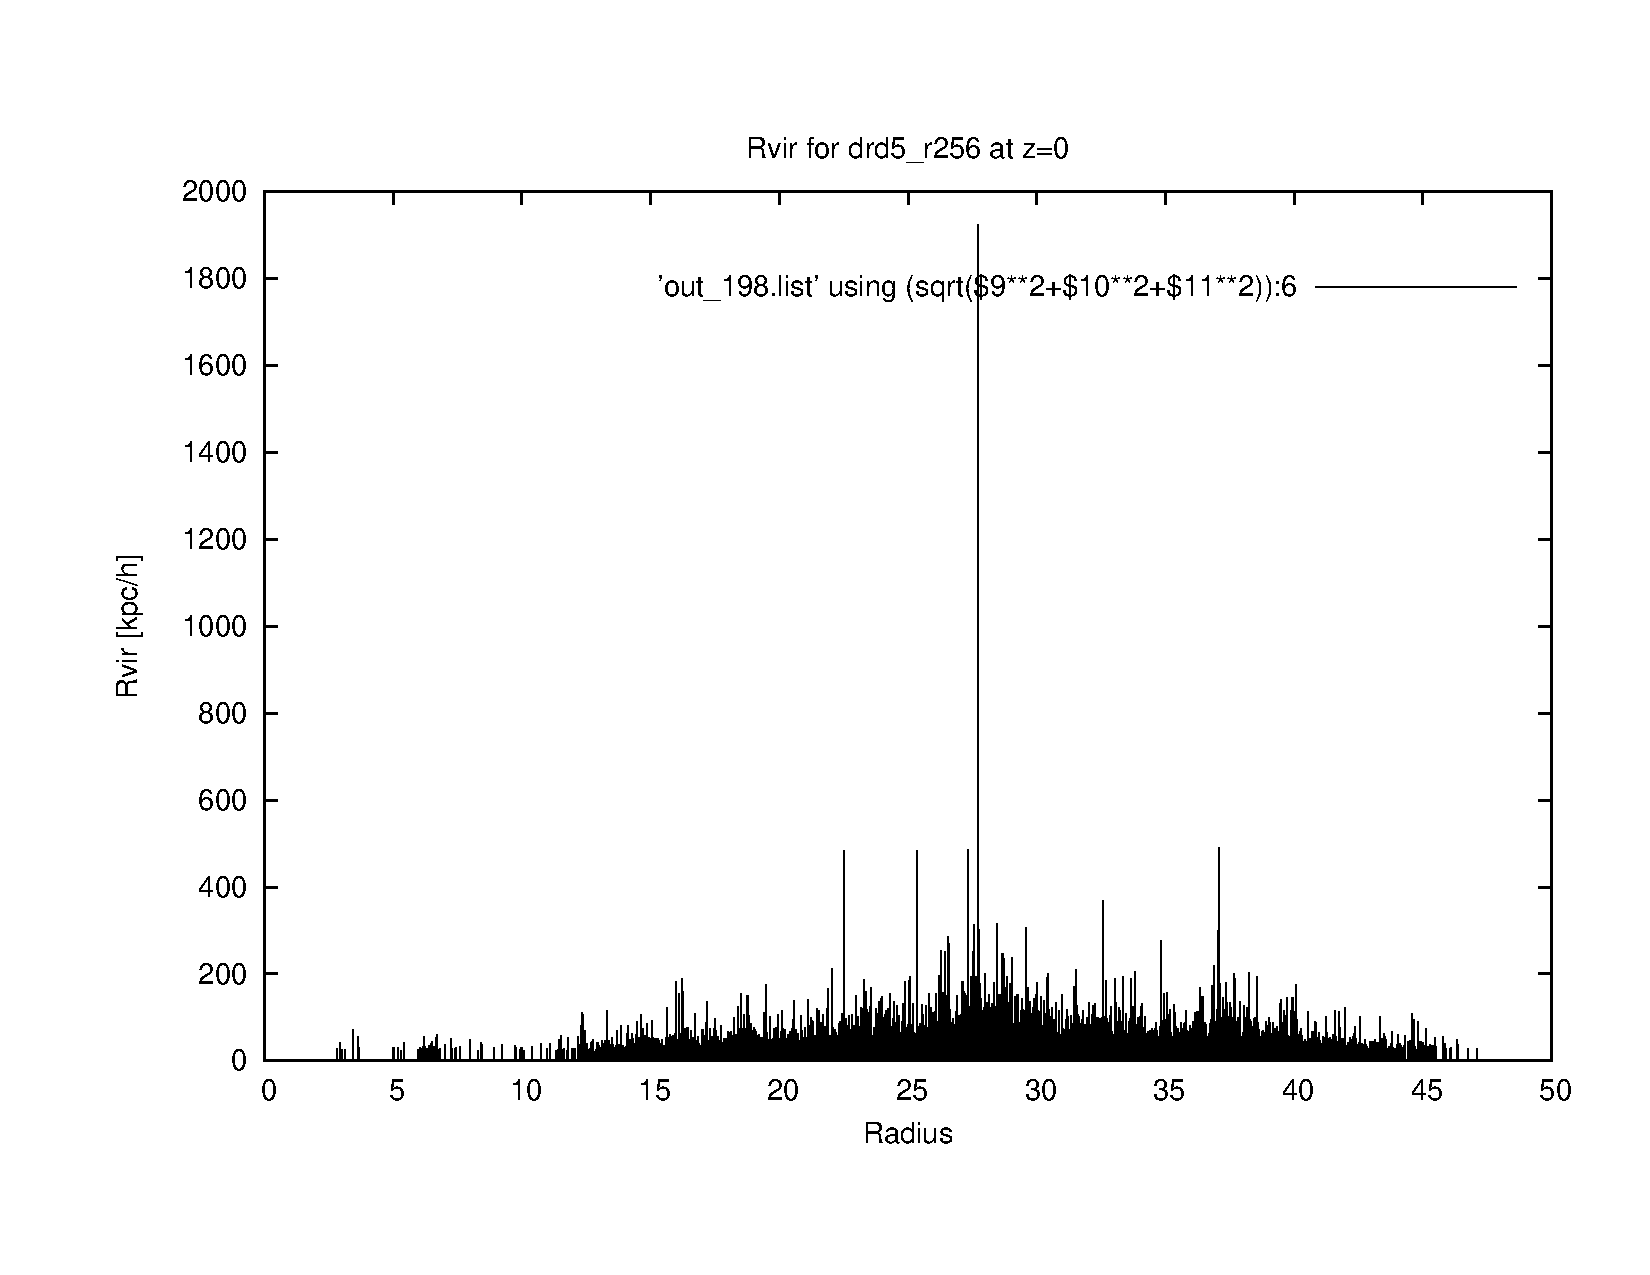
\includegraphics[scale=0.3]{drd5_r256/plot_rvir_z0.pdf}
% 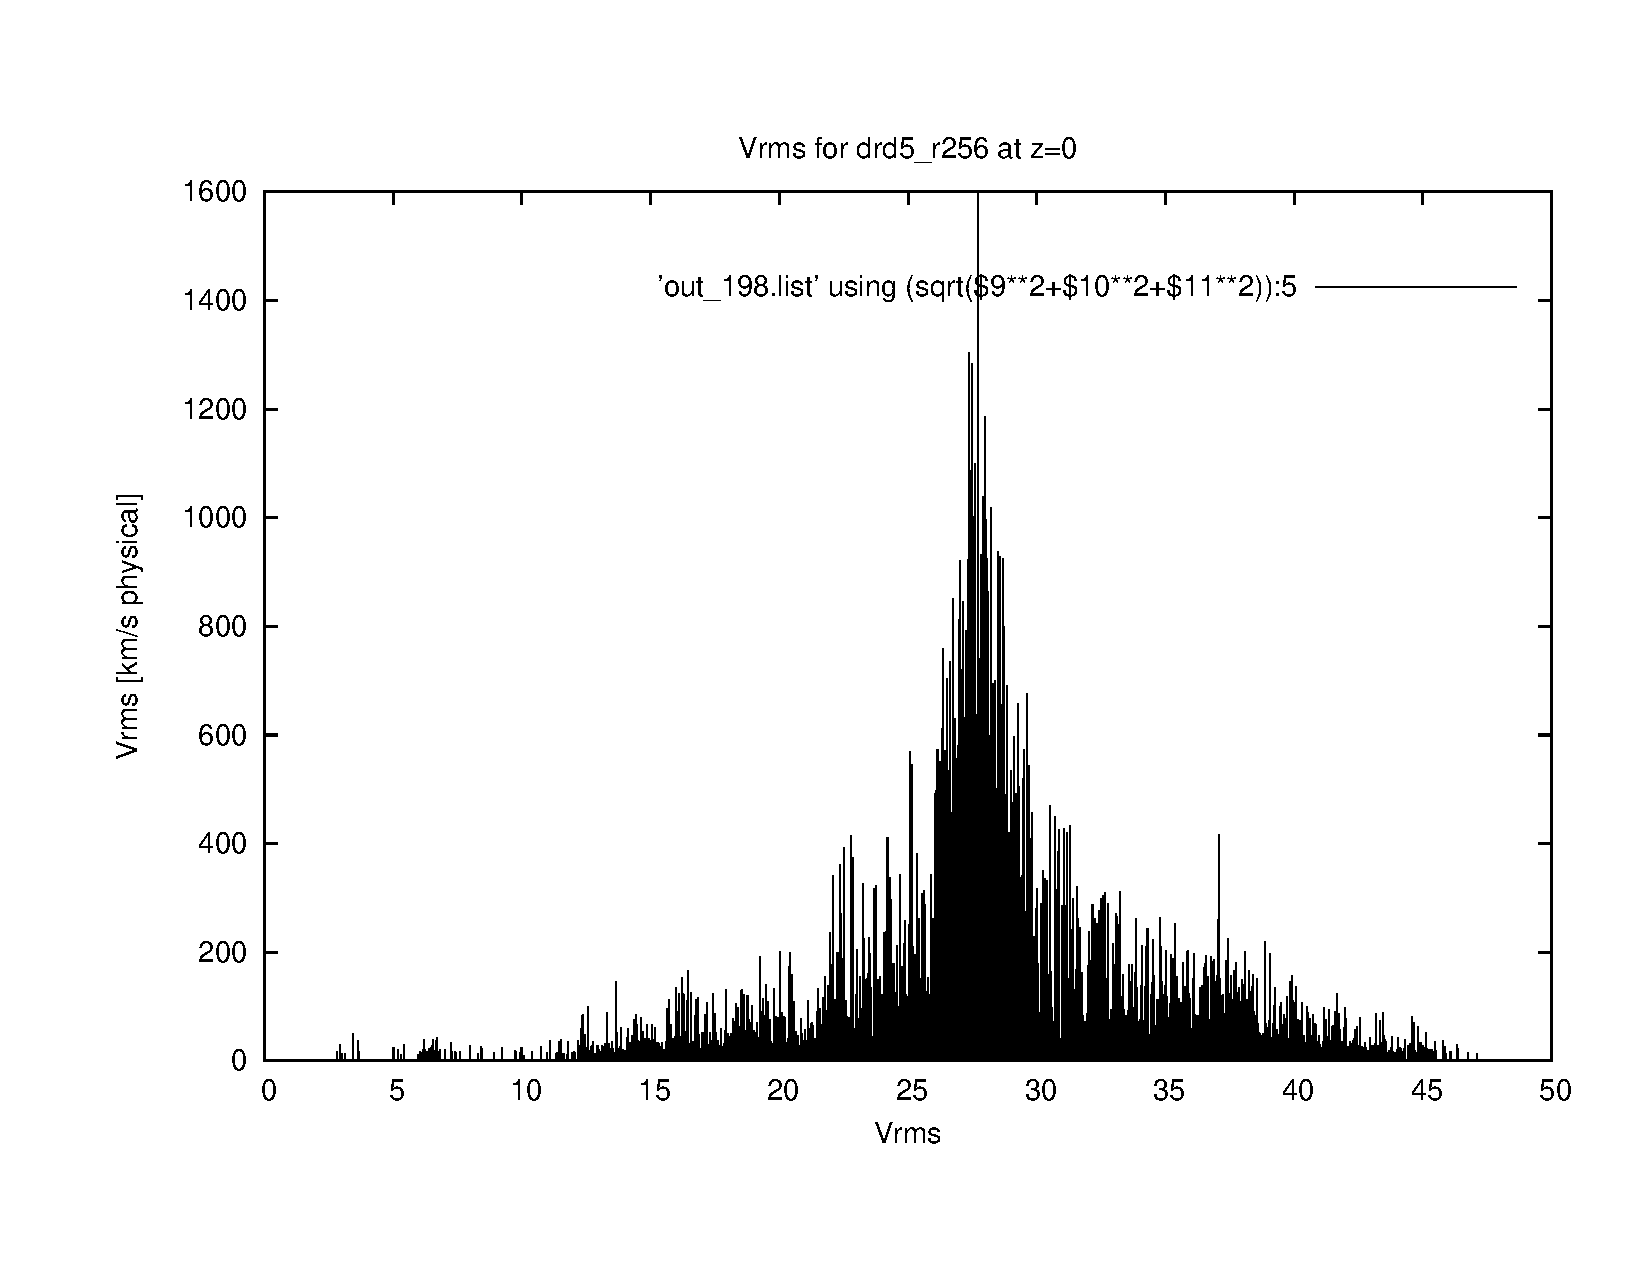
\includegraphics[scale=0.3]{drd5_r256/plot_vrms_z0.pdf}

\textsc{galacticussed} $\surd$  \\
galacticus running on SGE \\
$\rightarrow$ re-converted with bugfixed converter \\
tree copied to markus transfer \\
\textsc{galacticus}: 
\begin{verbatim}
Fatal error in Build_Descendent\_Pointers():
failed to find descendent node: 5546454 of 5522259
galacticus.sh: line 67: 25689 Aborted  
\end{verbatim}
\textsc{consistenttreed} $\surd$  \\ 
\textsc{rockstarred} $\surd$ \\ 

% 
%
%
%
%
%
%
%

\newpage
\subsection{drd5\_r256\_2 (+ major merger in progress)} 

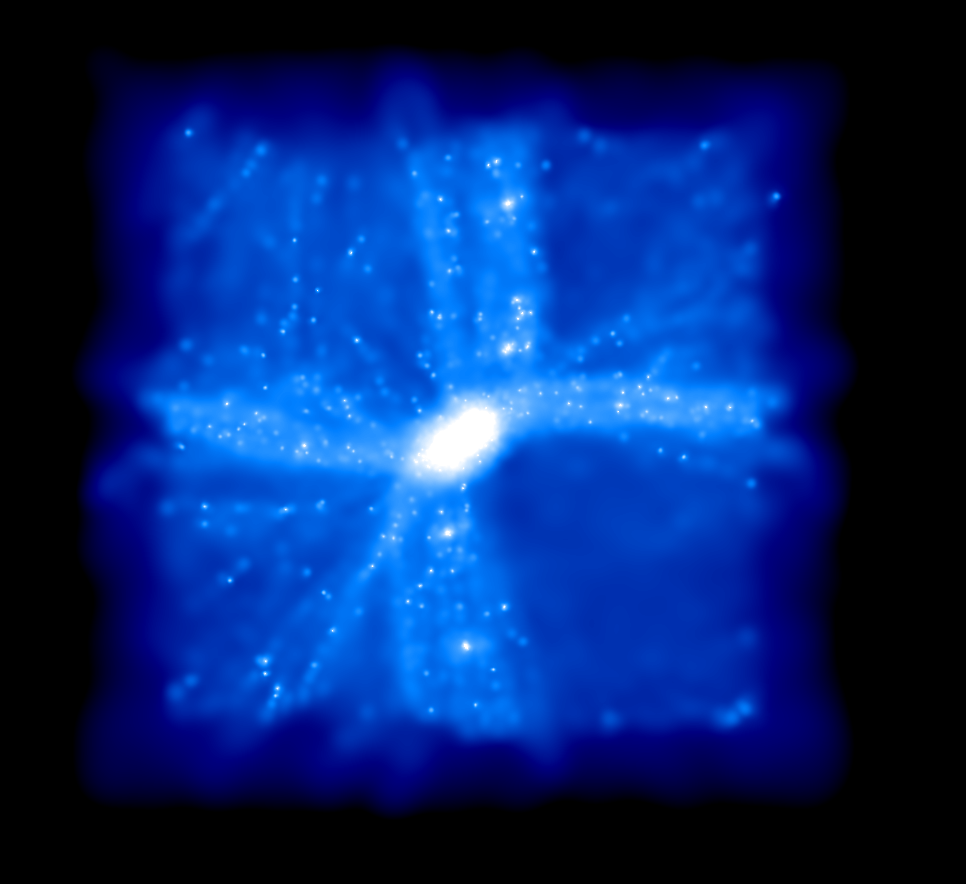
\includegraphics[scale=0.2]{drd5_r256_2/1.png} 
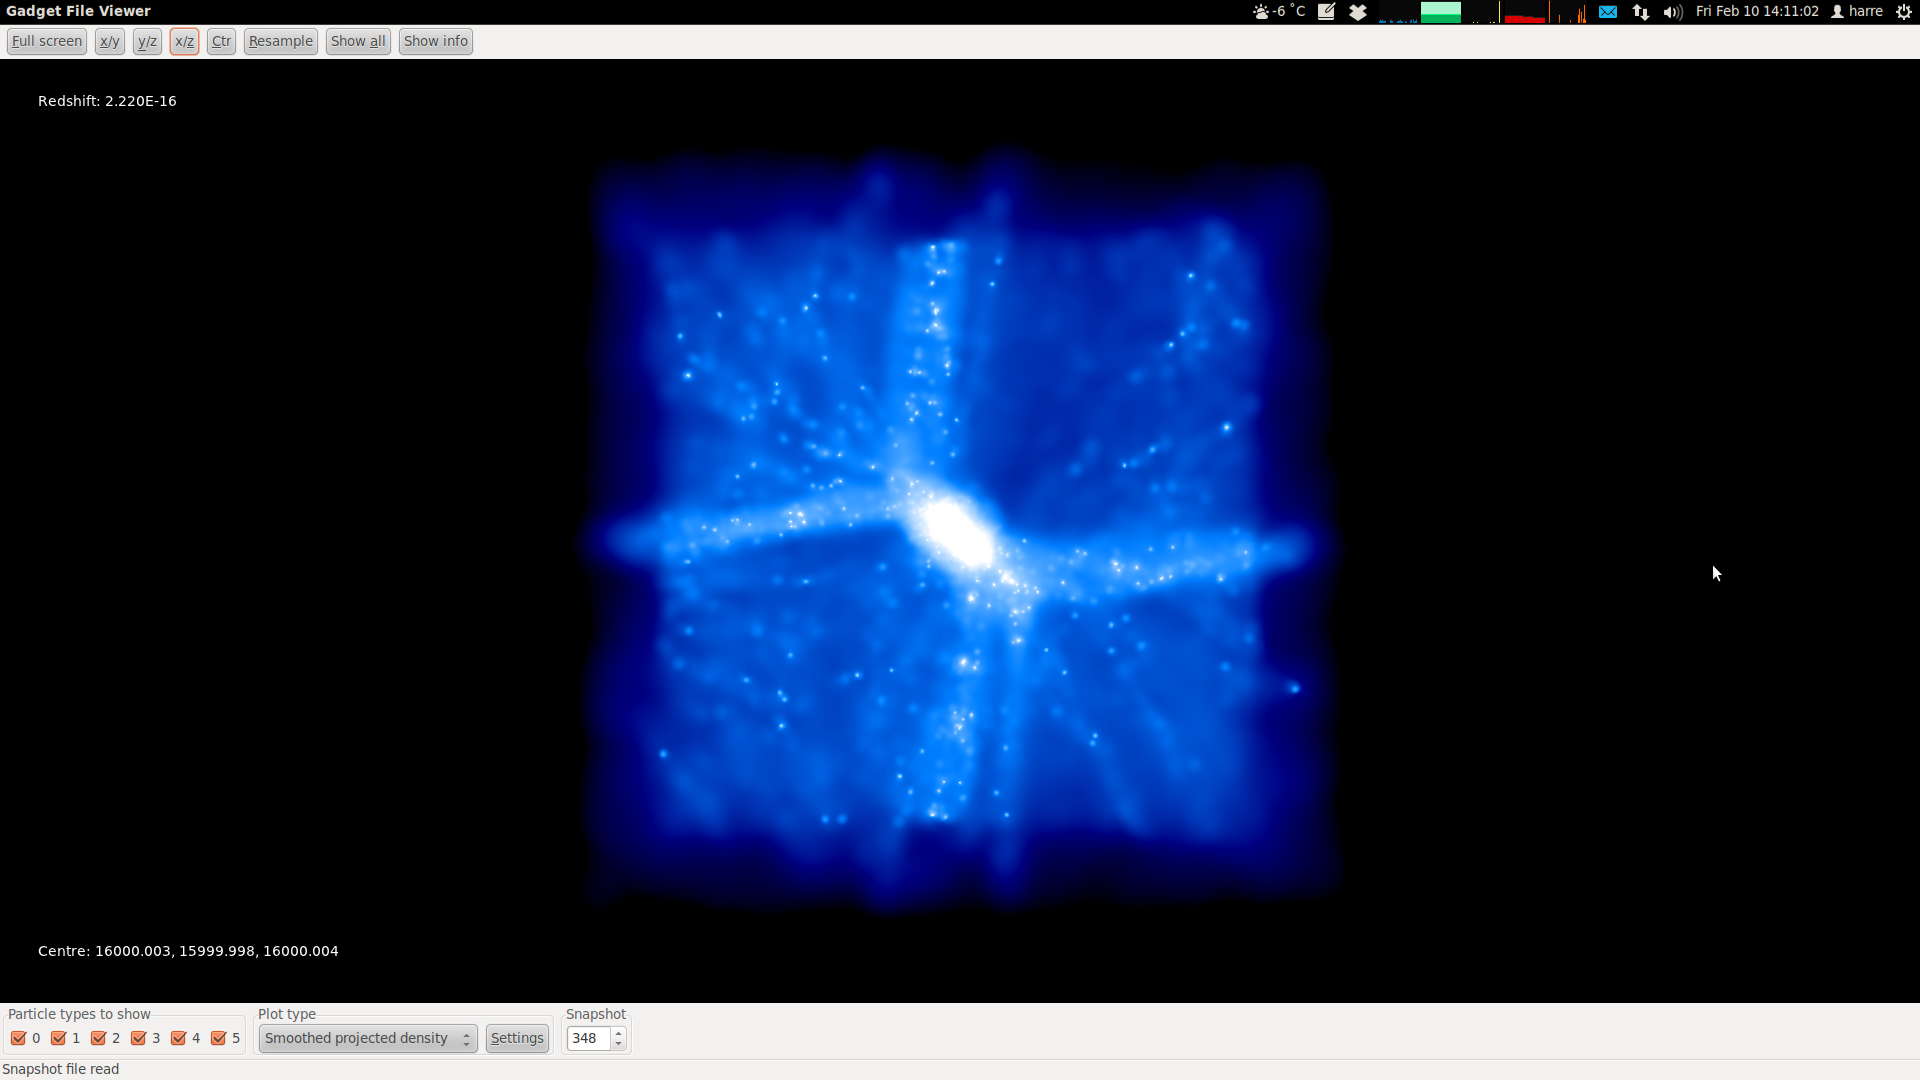
\includegraphics[scale=0.2]{drd5_r256_2/2.png} 

\textbf{Evolution:} \\
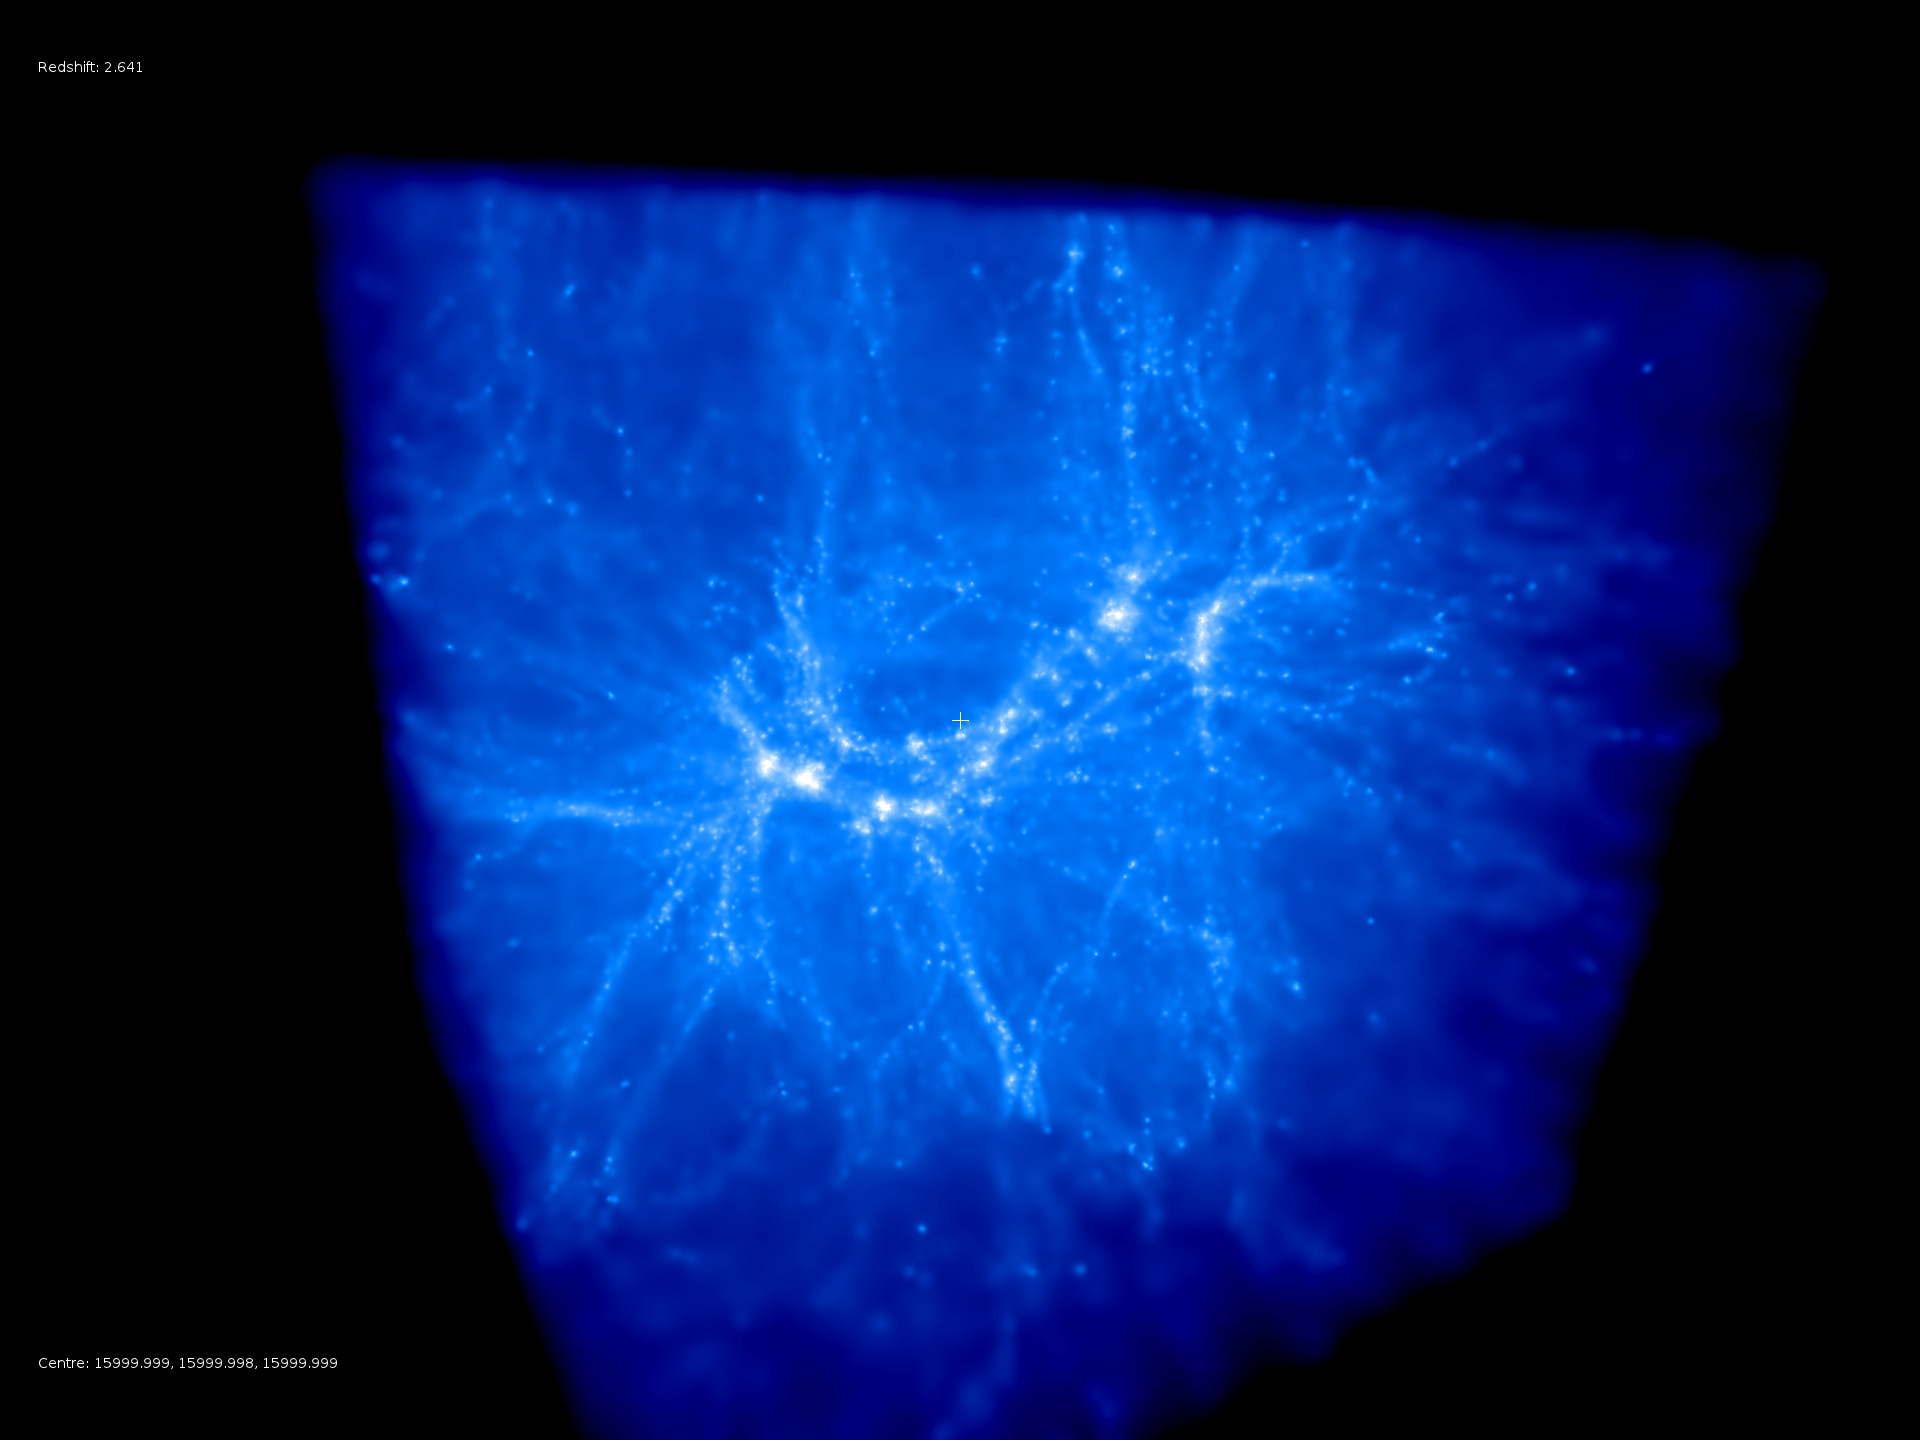
\includegraphics[scale=0.1]{drd5_r256_2/62.jpg} 
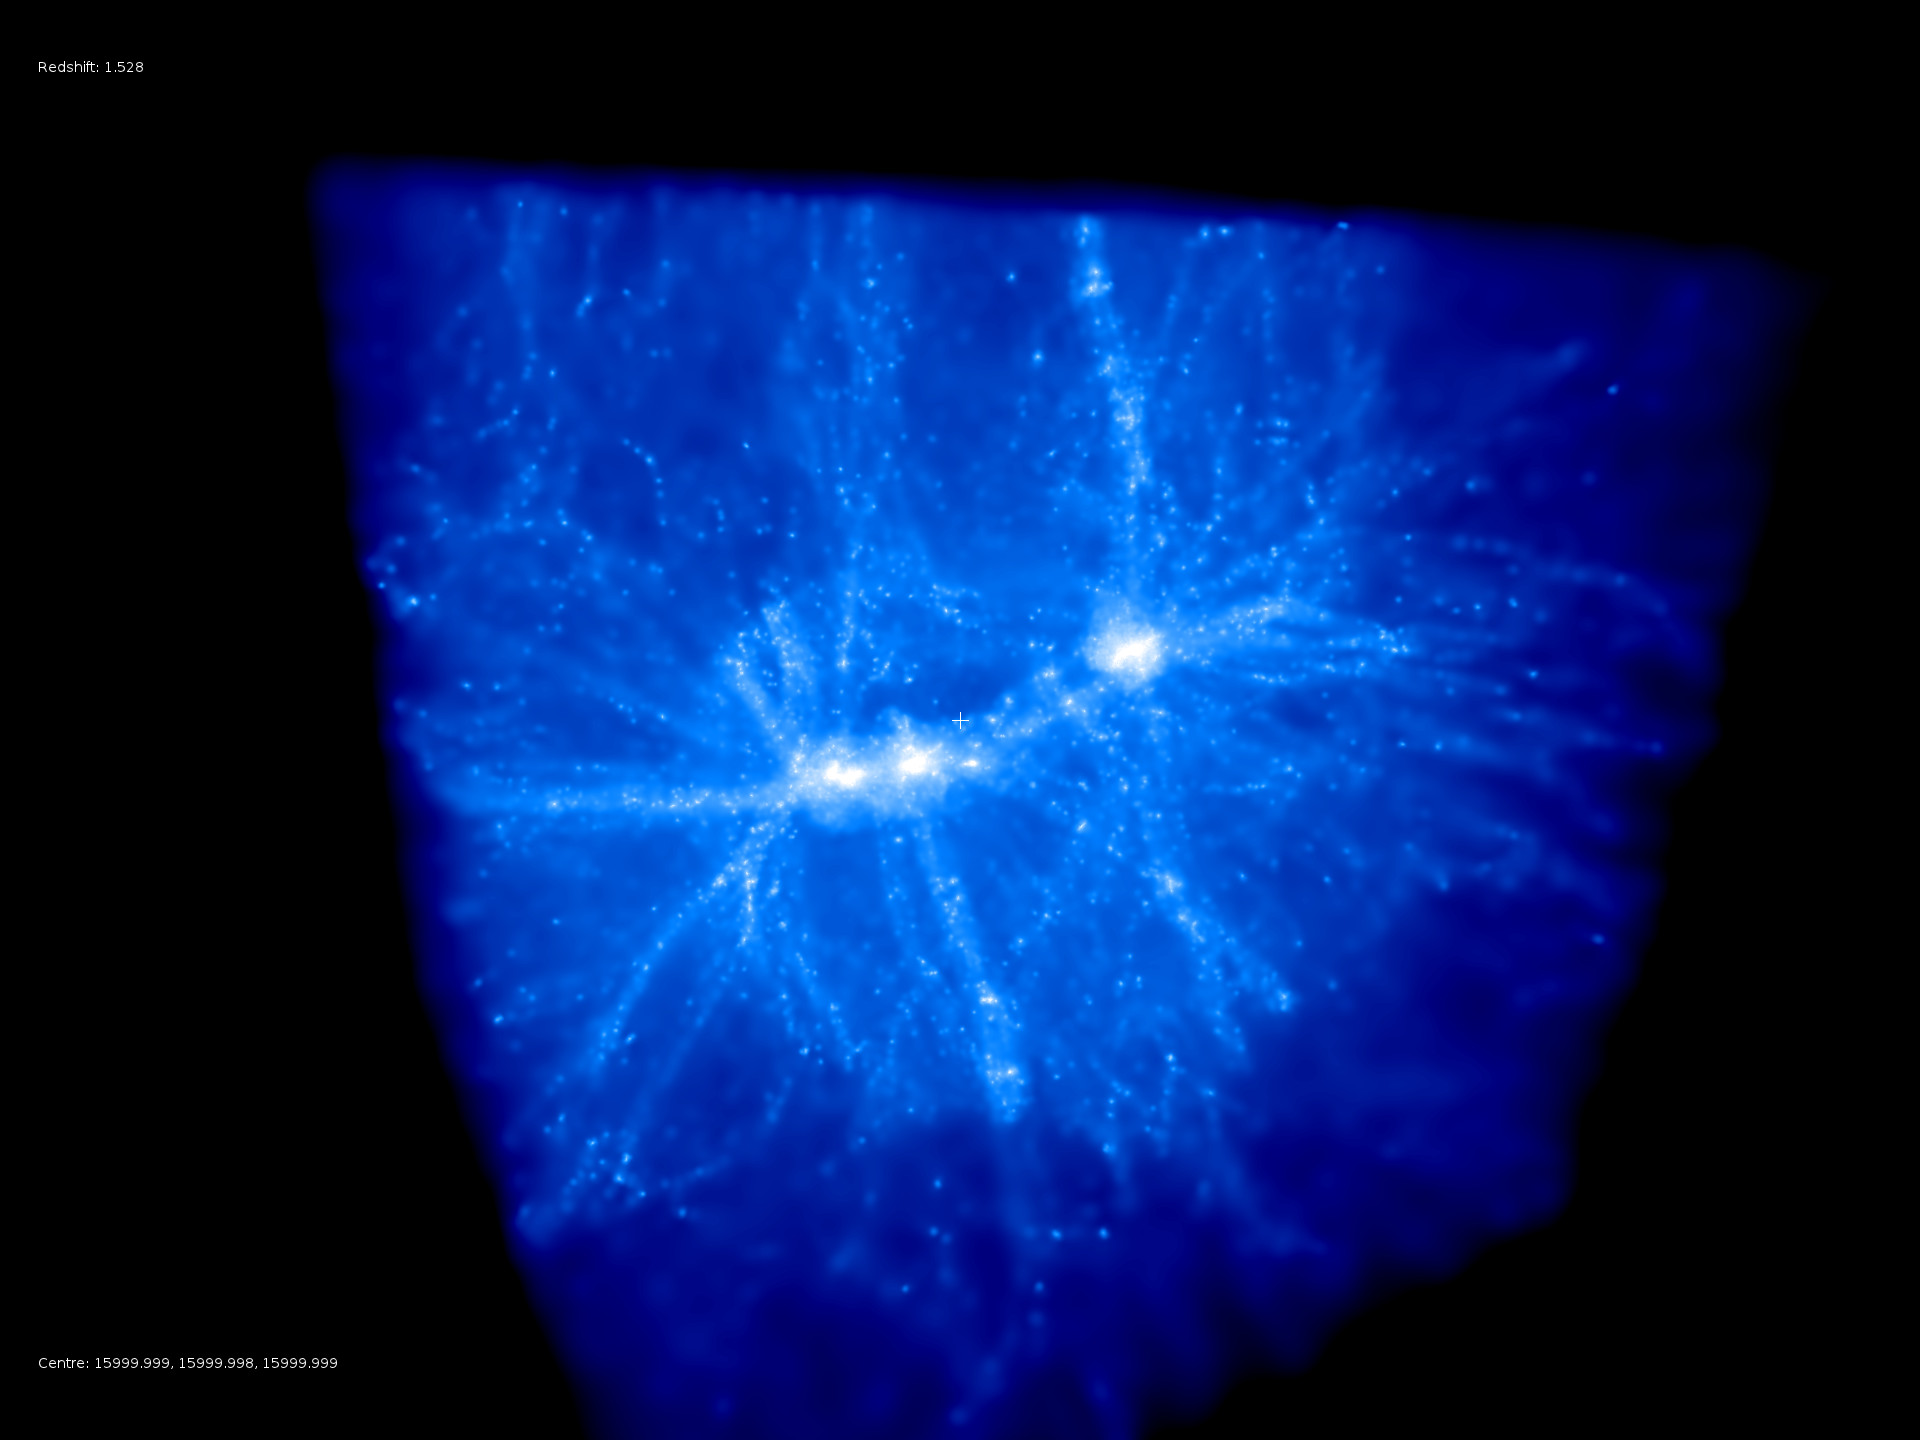
\includegraphics[scale=0.1]{drd5_r256_2/107.jpg} 
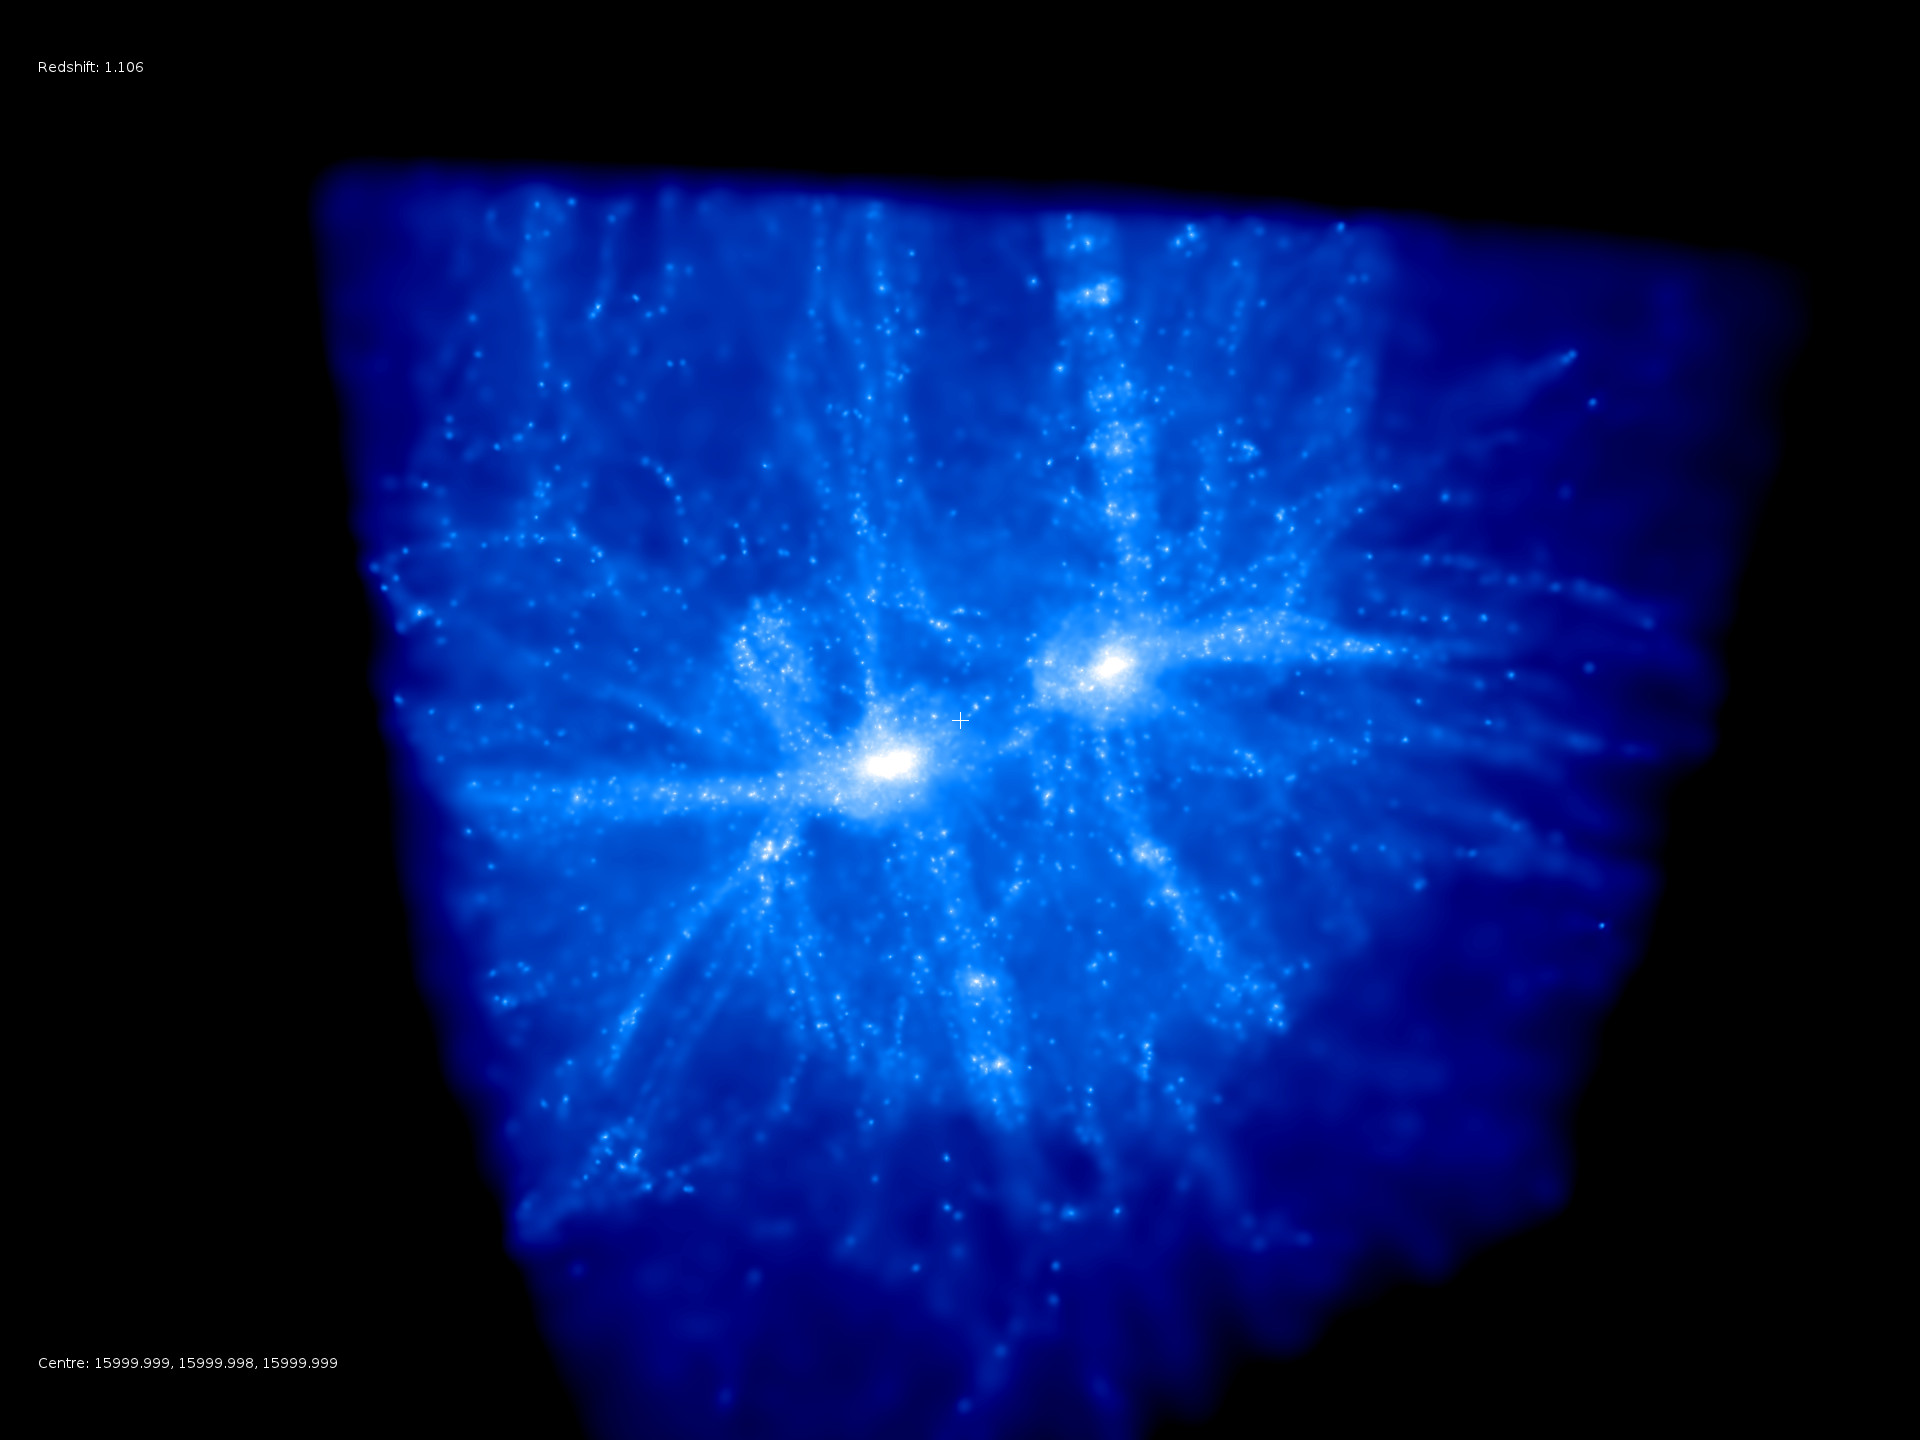
\includegraphics[scale=0.1]{drd5_r256_2/139.jpg} 
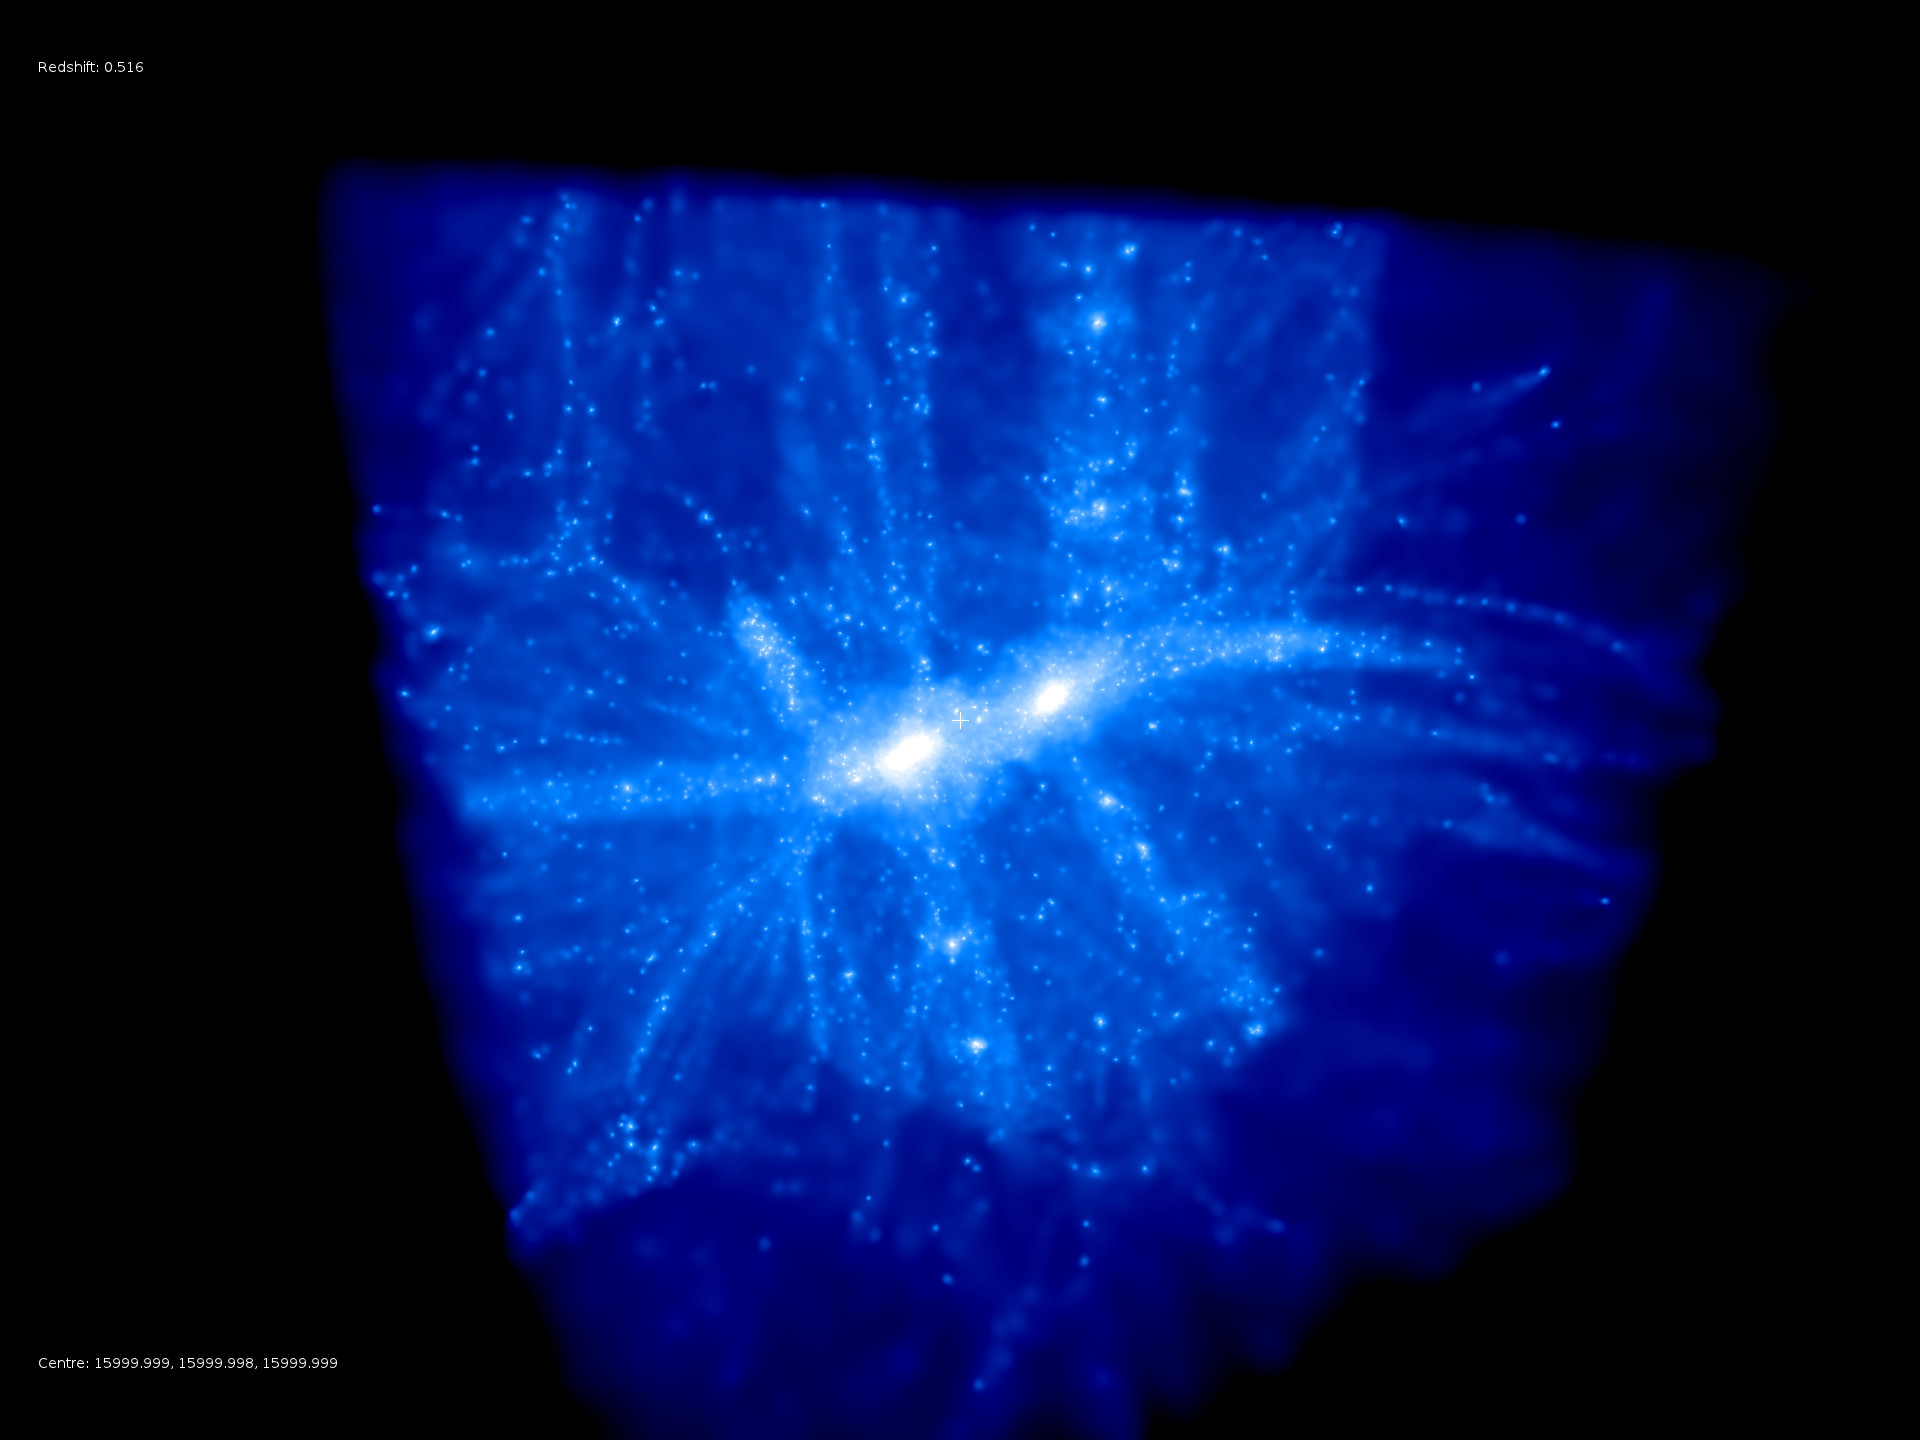
\includegraphics[scale=0.1]{drd5_r256_2/216.jpg} 
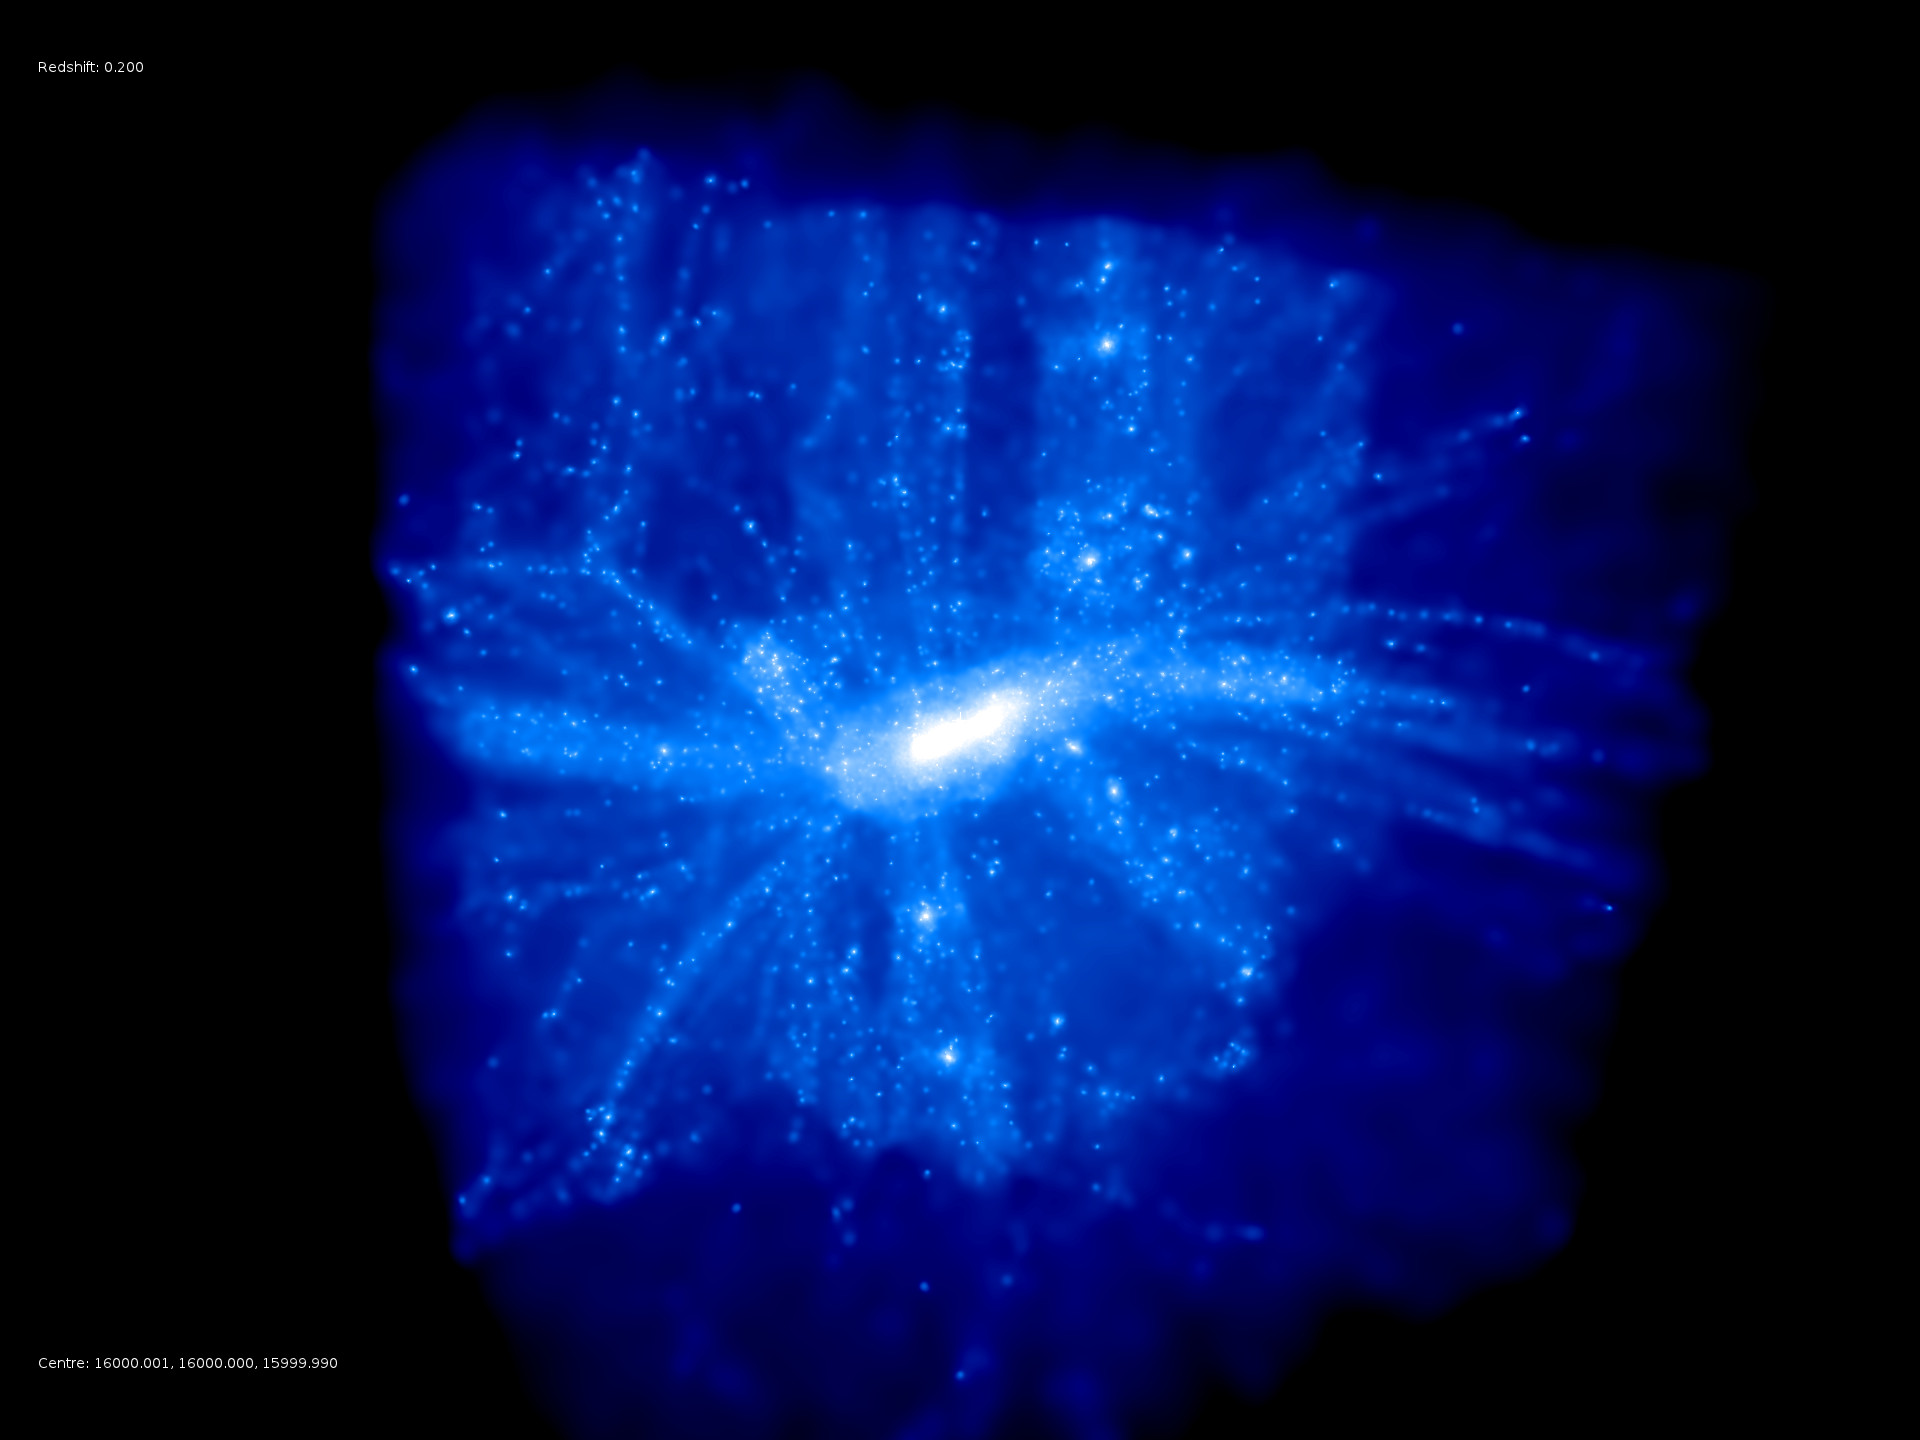
\includegraphics[scale=0.1]{drd5_r256_2/286.jpg} 
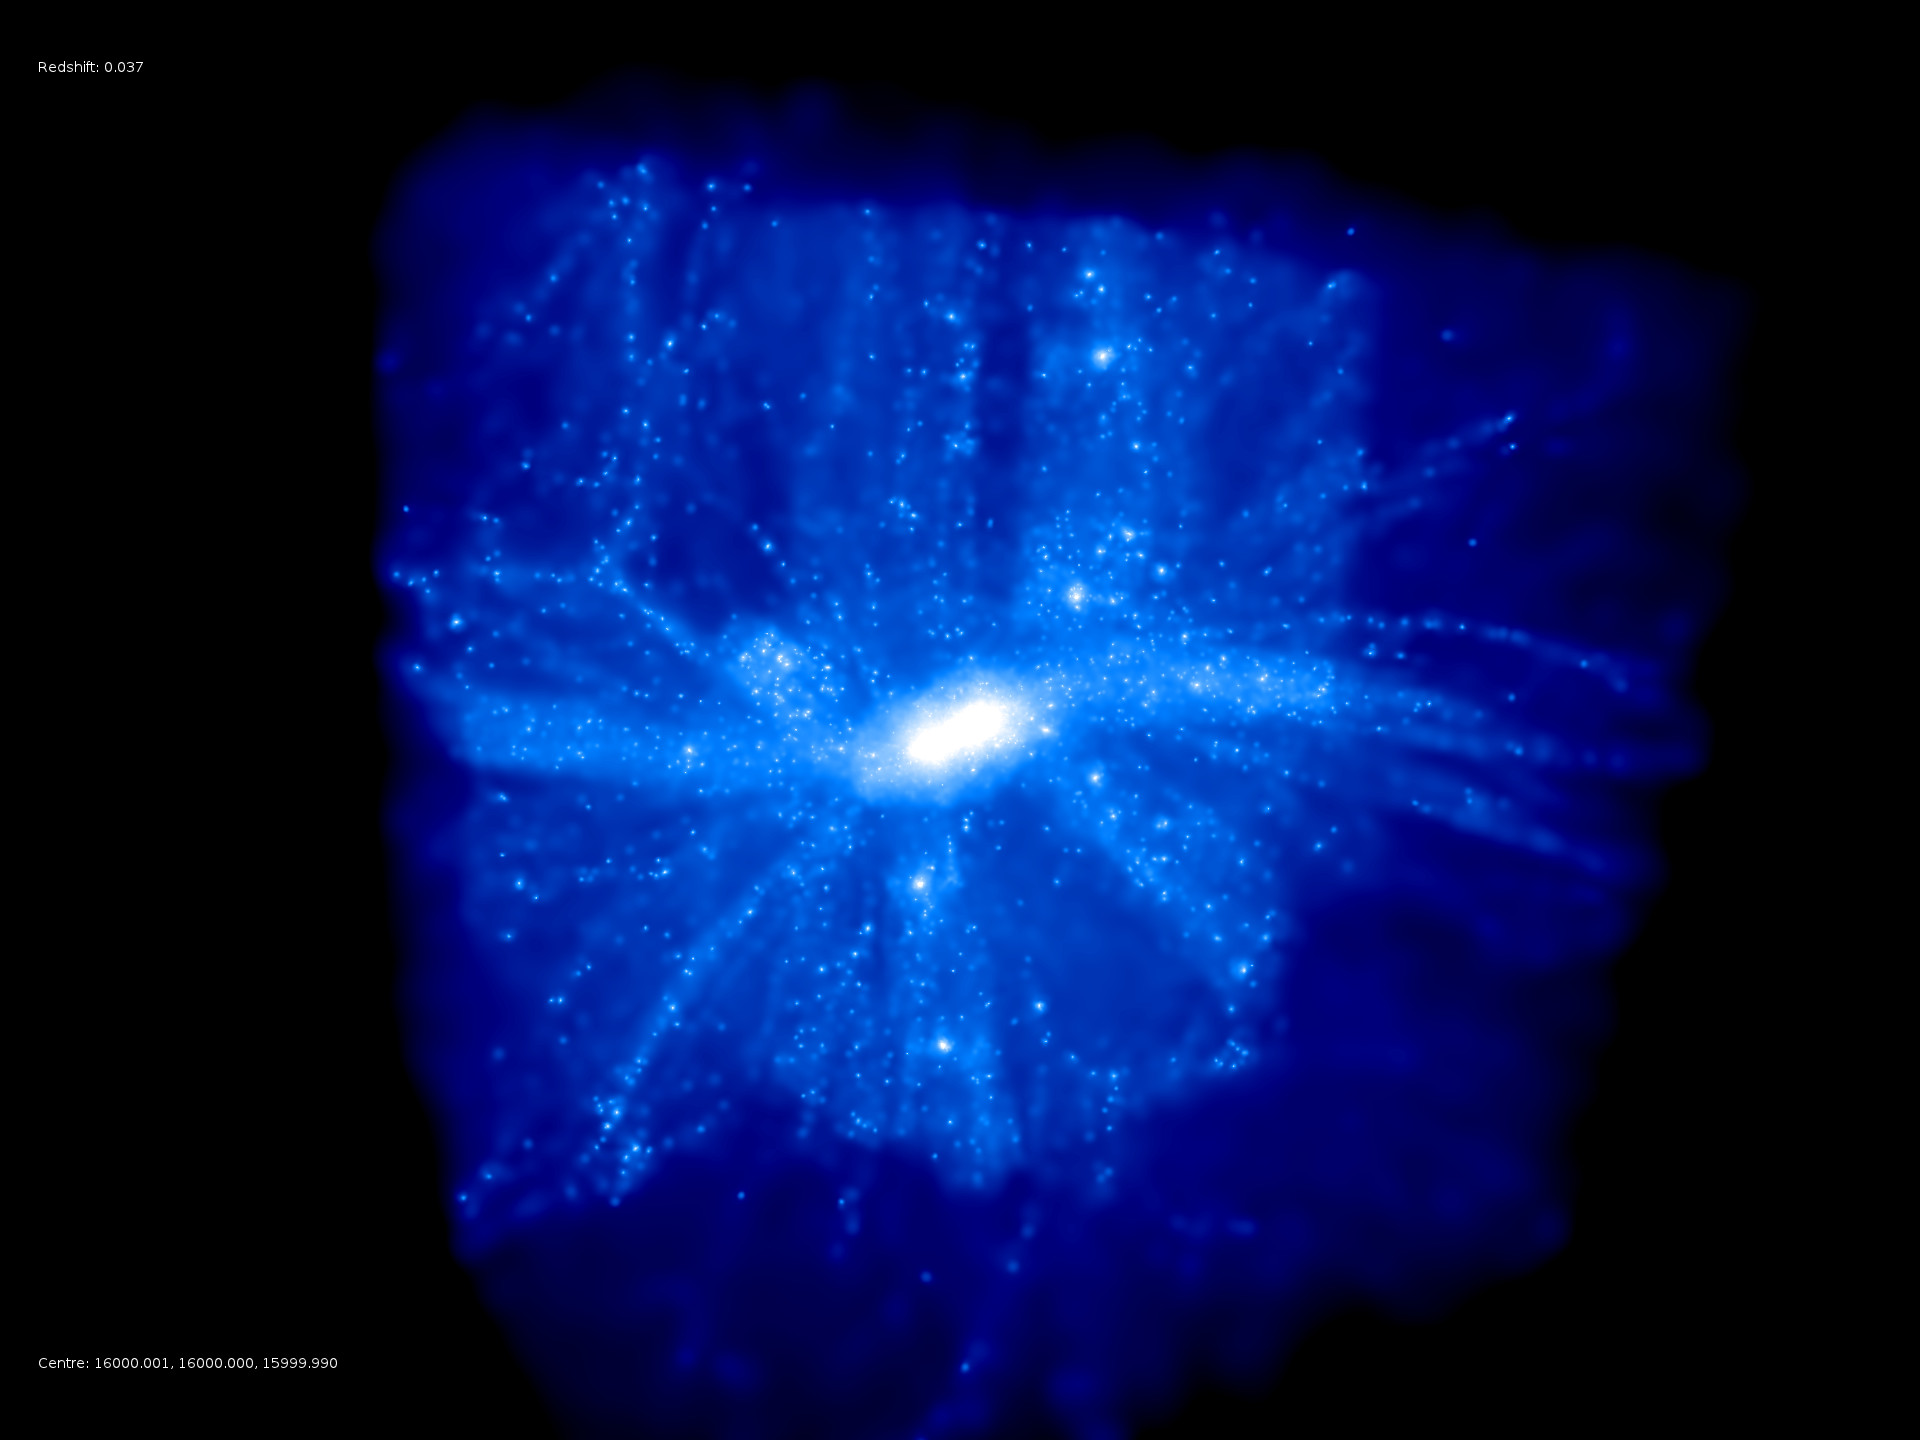
\includegraphics[scale=0.1]{drd5_r256_2/335.jpg} 

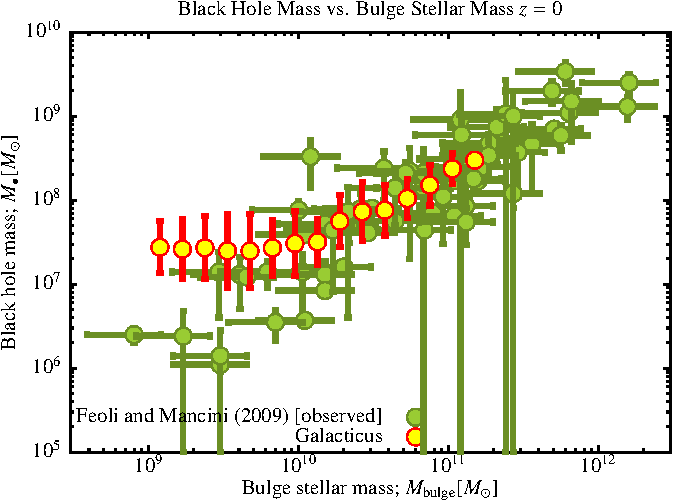
\includegraphics[scale=0.6]{drd5_r256_2/Plot_Black_Hole_vs_Bulge_Mass.pdf}
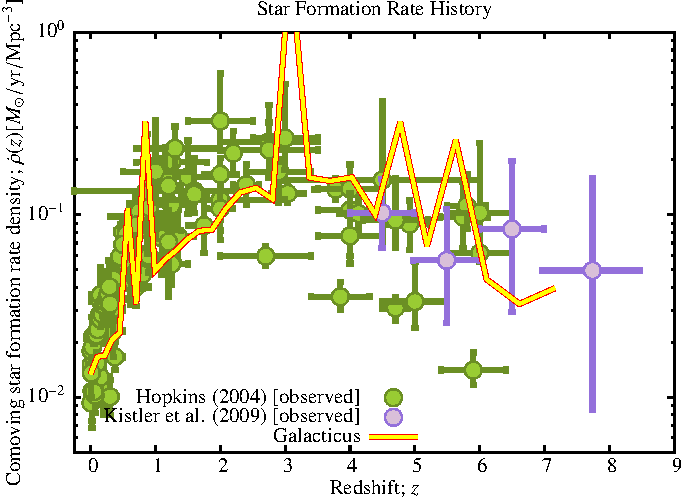
\includegraphics[scale=0.6]{drd5_r256_2/Plot_Star_Formation_History.pdf}
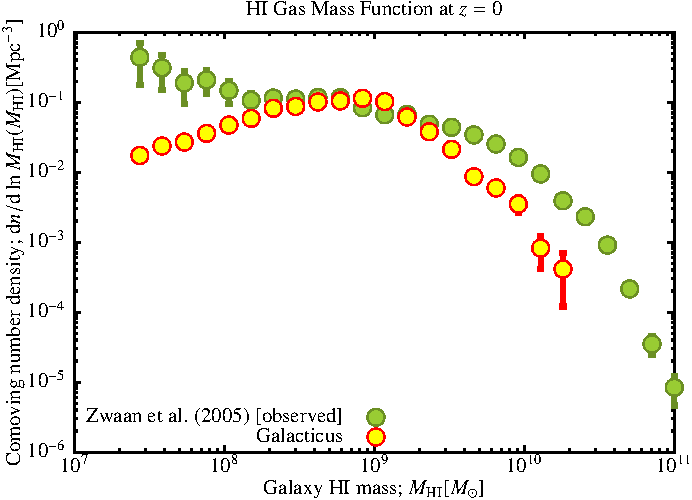
\includegraphics[scale=0.6]{drd5_r256_2/Plot_HI_Mass_Function.pdf}

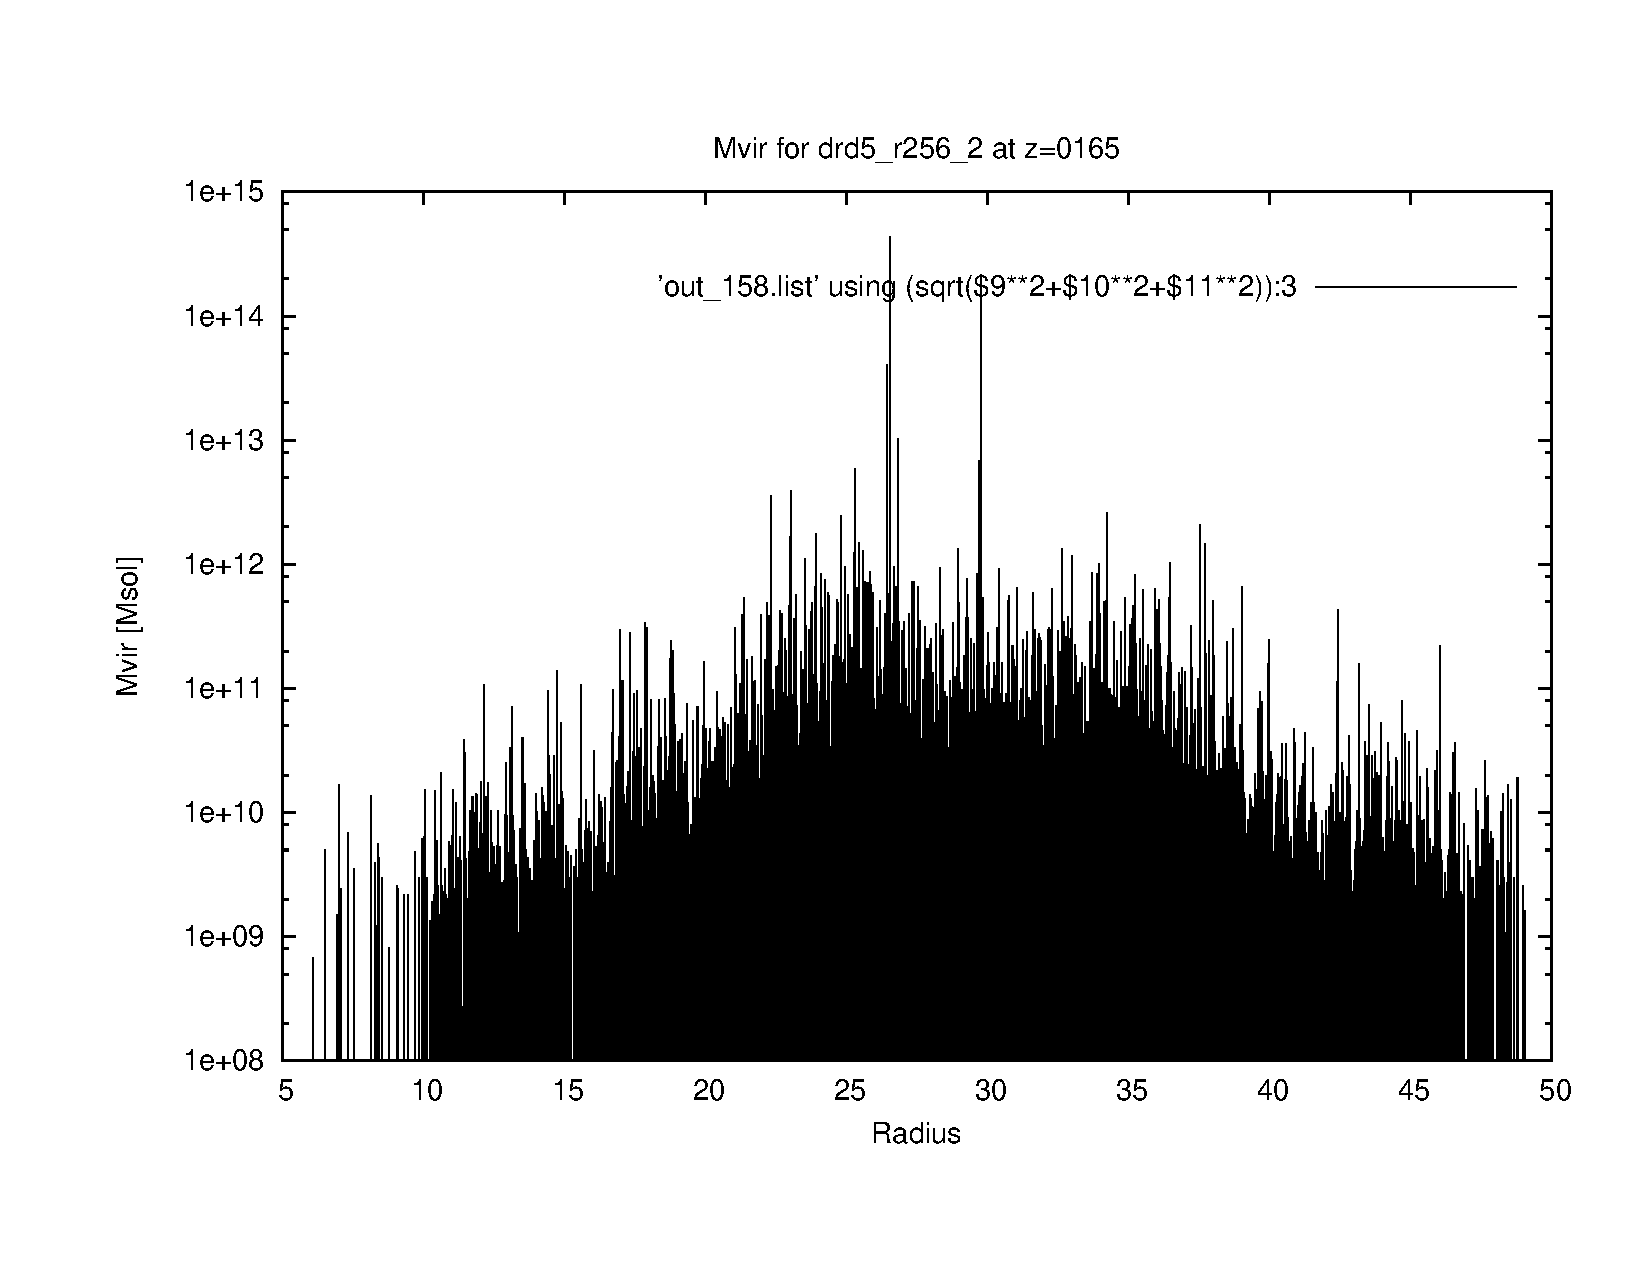
\includegraphics[scale=0.3]{drd5_r256_2/plot_mvir_z0165.pdf}
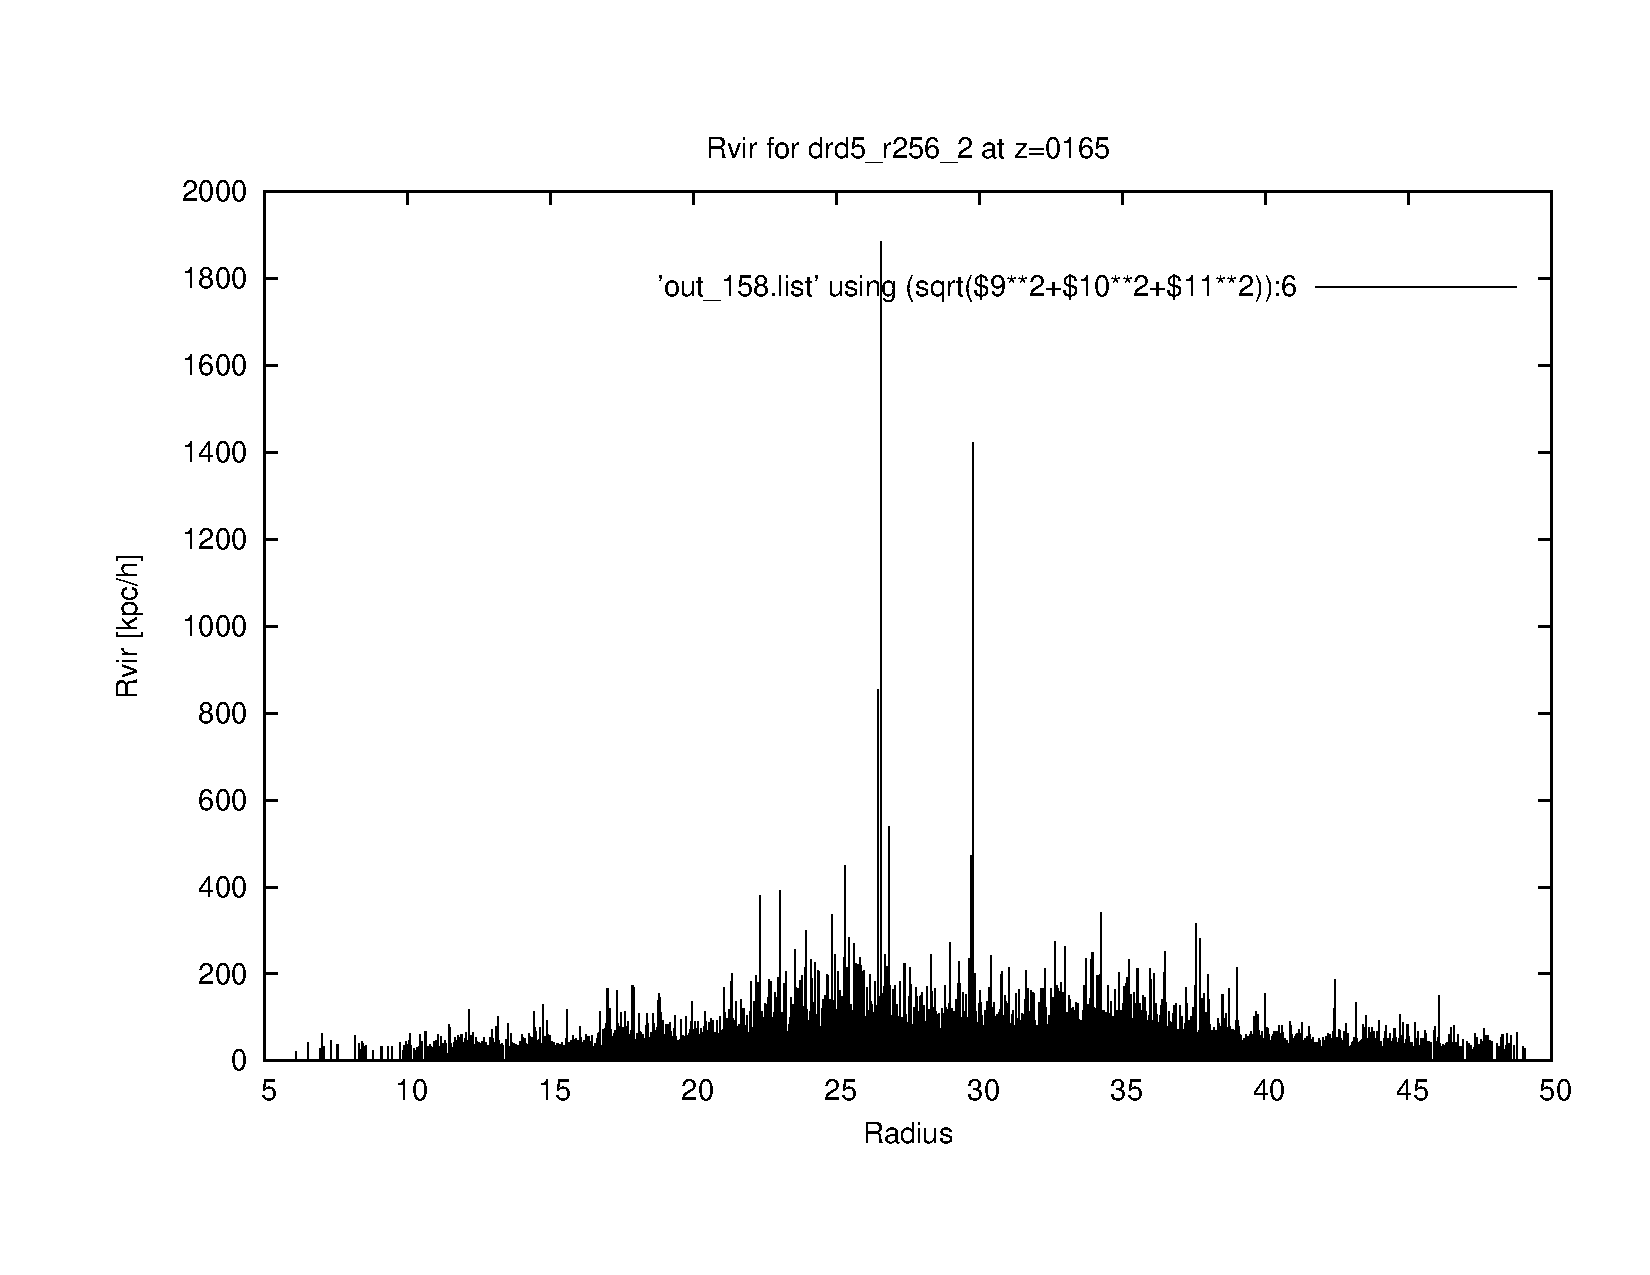
\includegraphics[scale=0.3]{drd5_r256_2/plot_rvir_z0165.pdf}
% 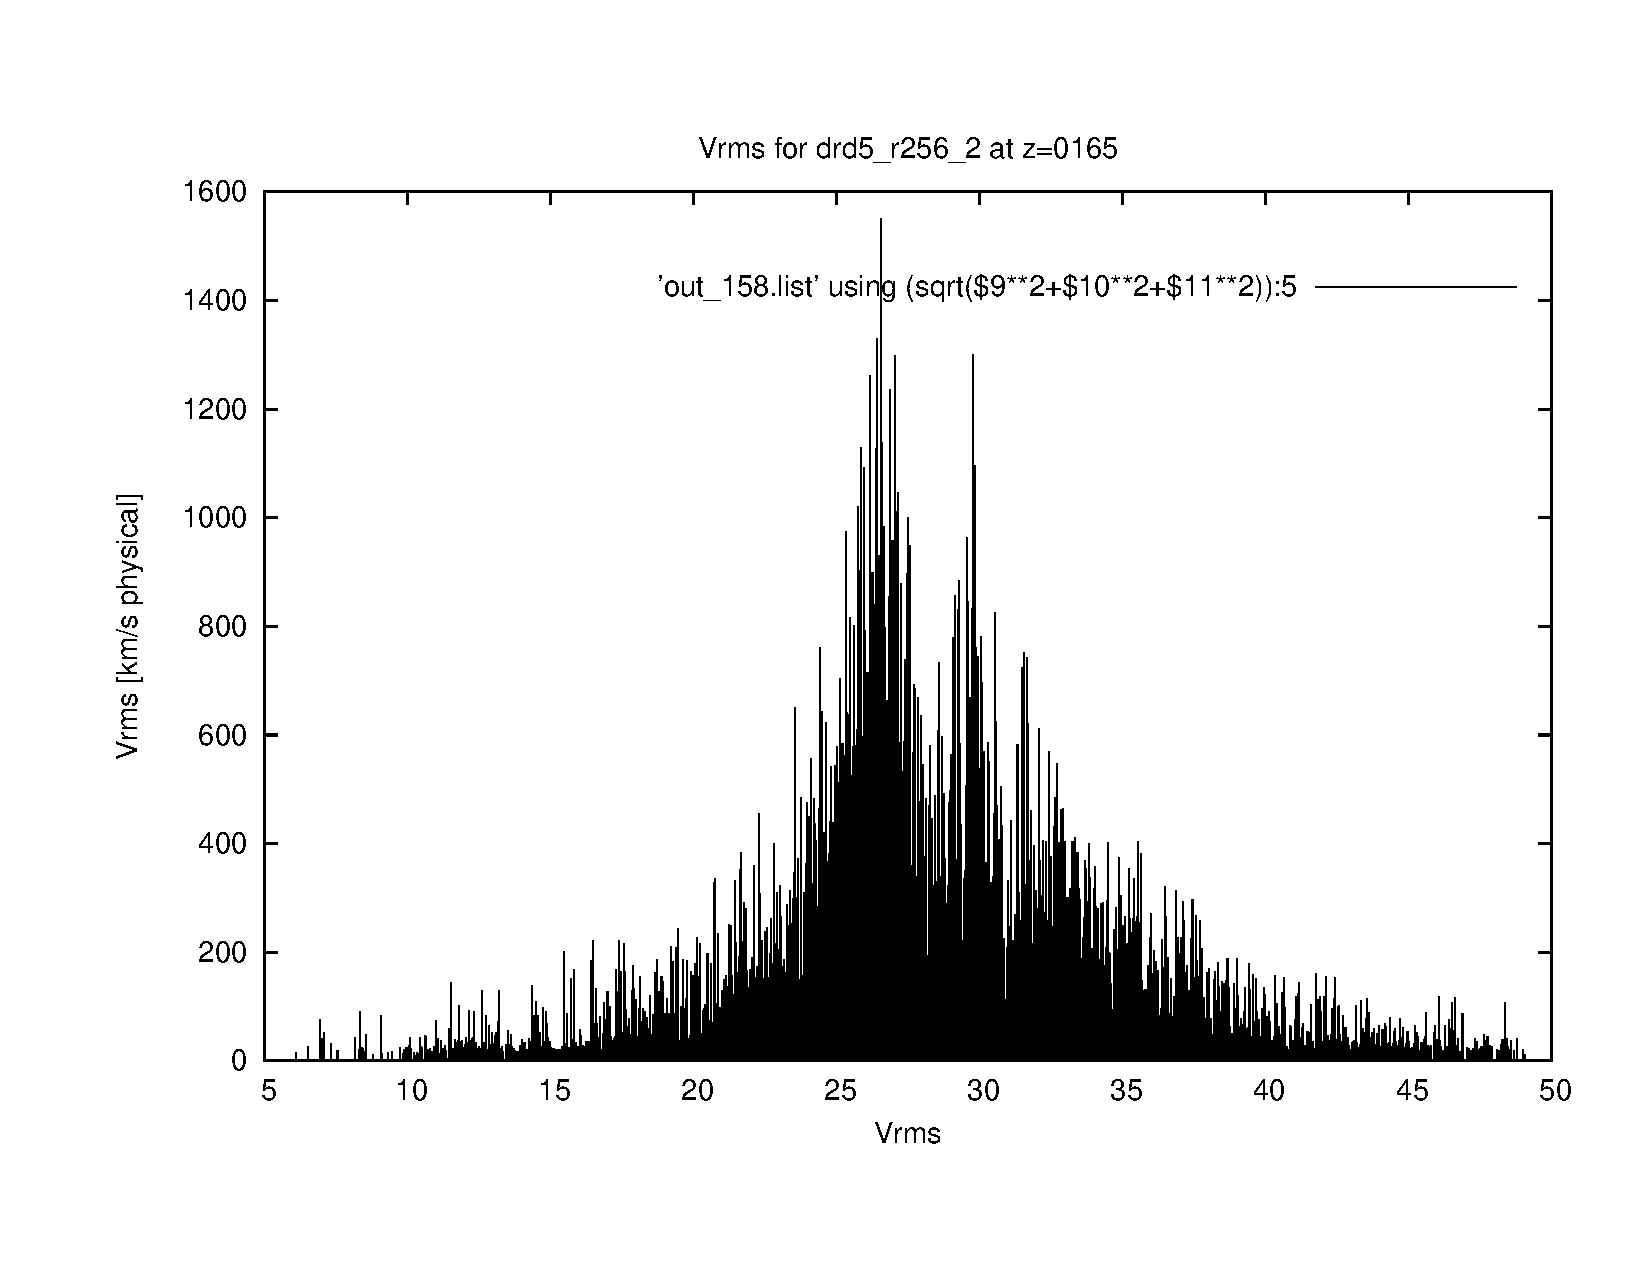
\includegraphics[scale=0.3]{drd5_r256_2/plot_vrms_z0165.pdf} 
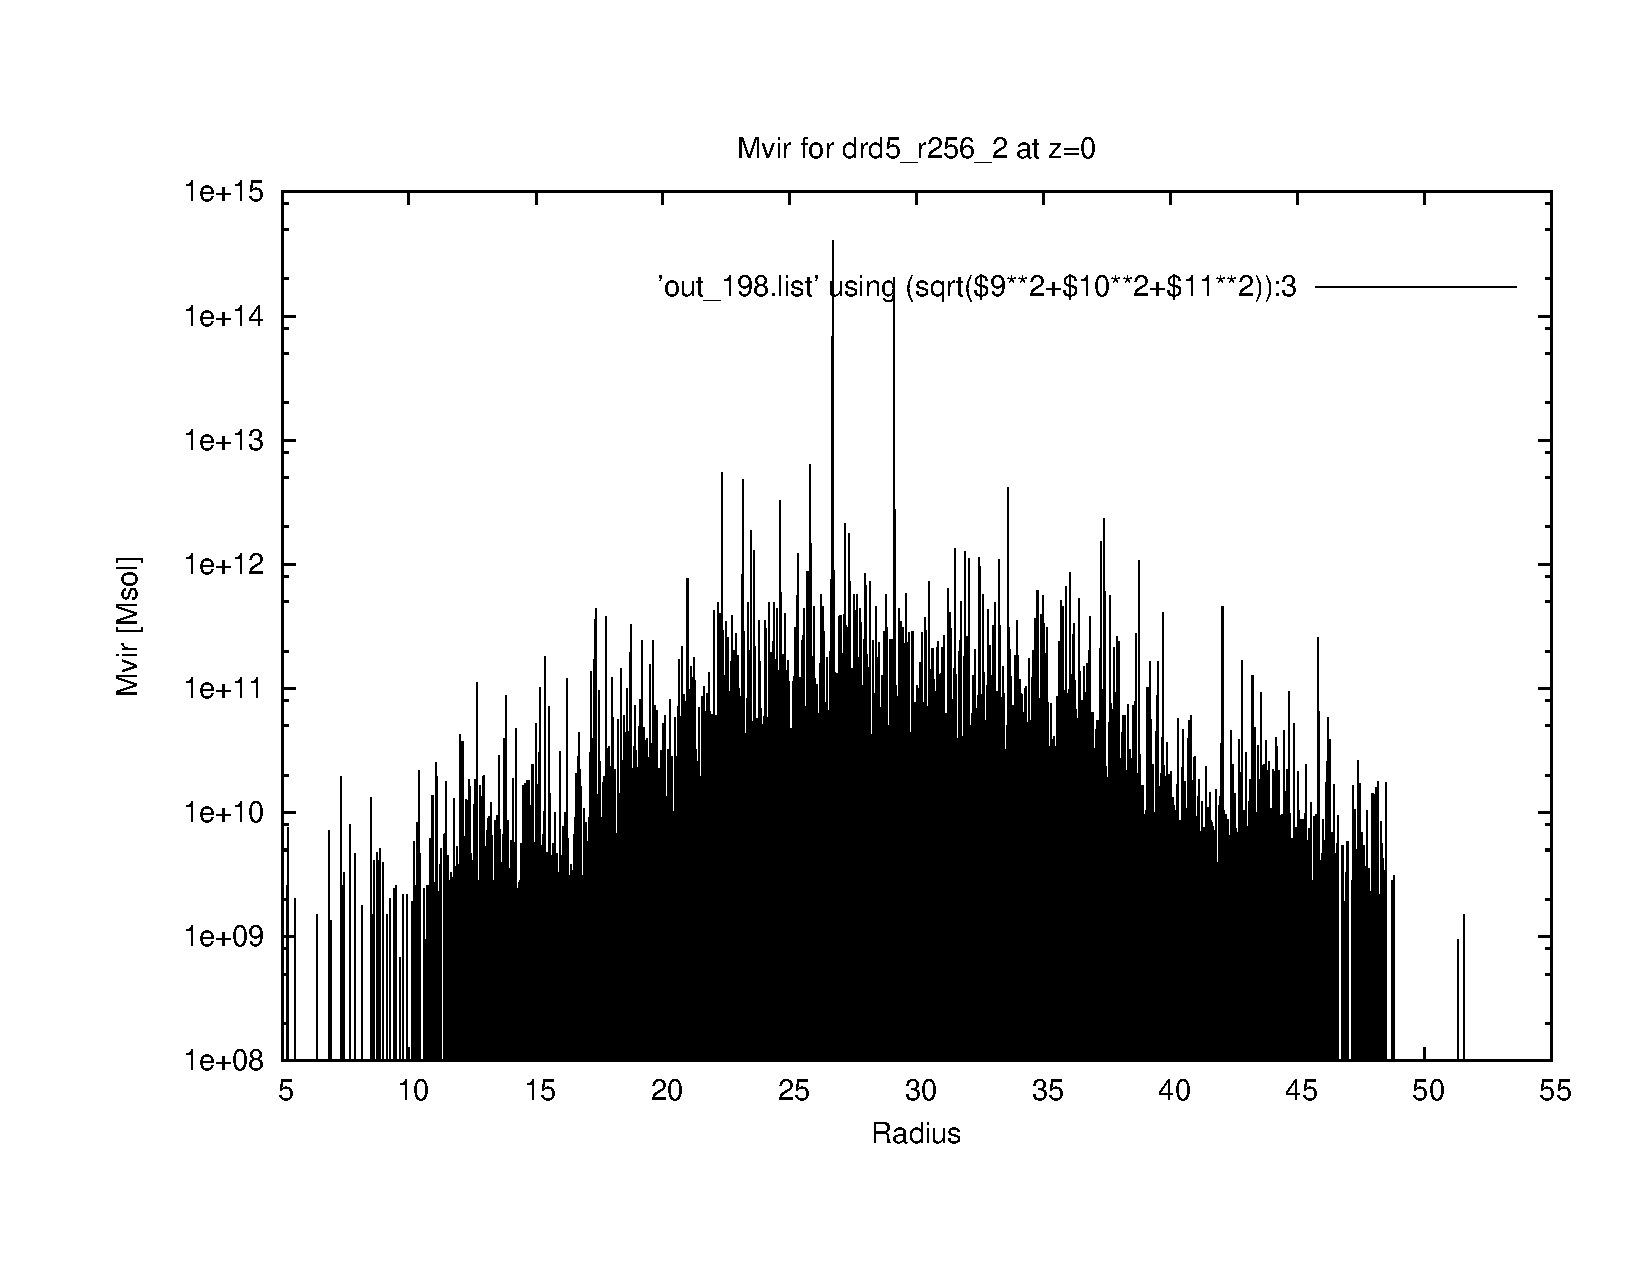
\includegraphics[scale=0.3]{drd5_r256_2/plot_mvir_z0.pdf}
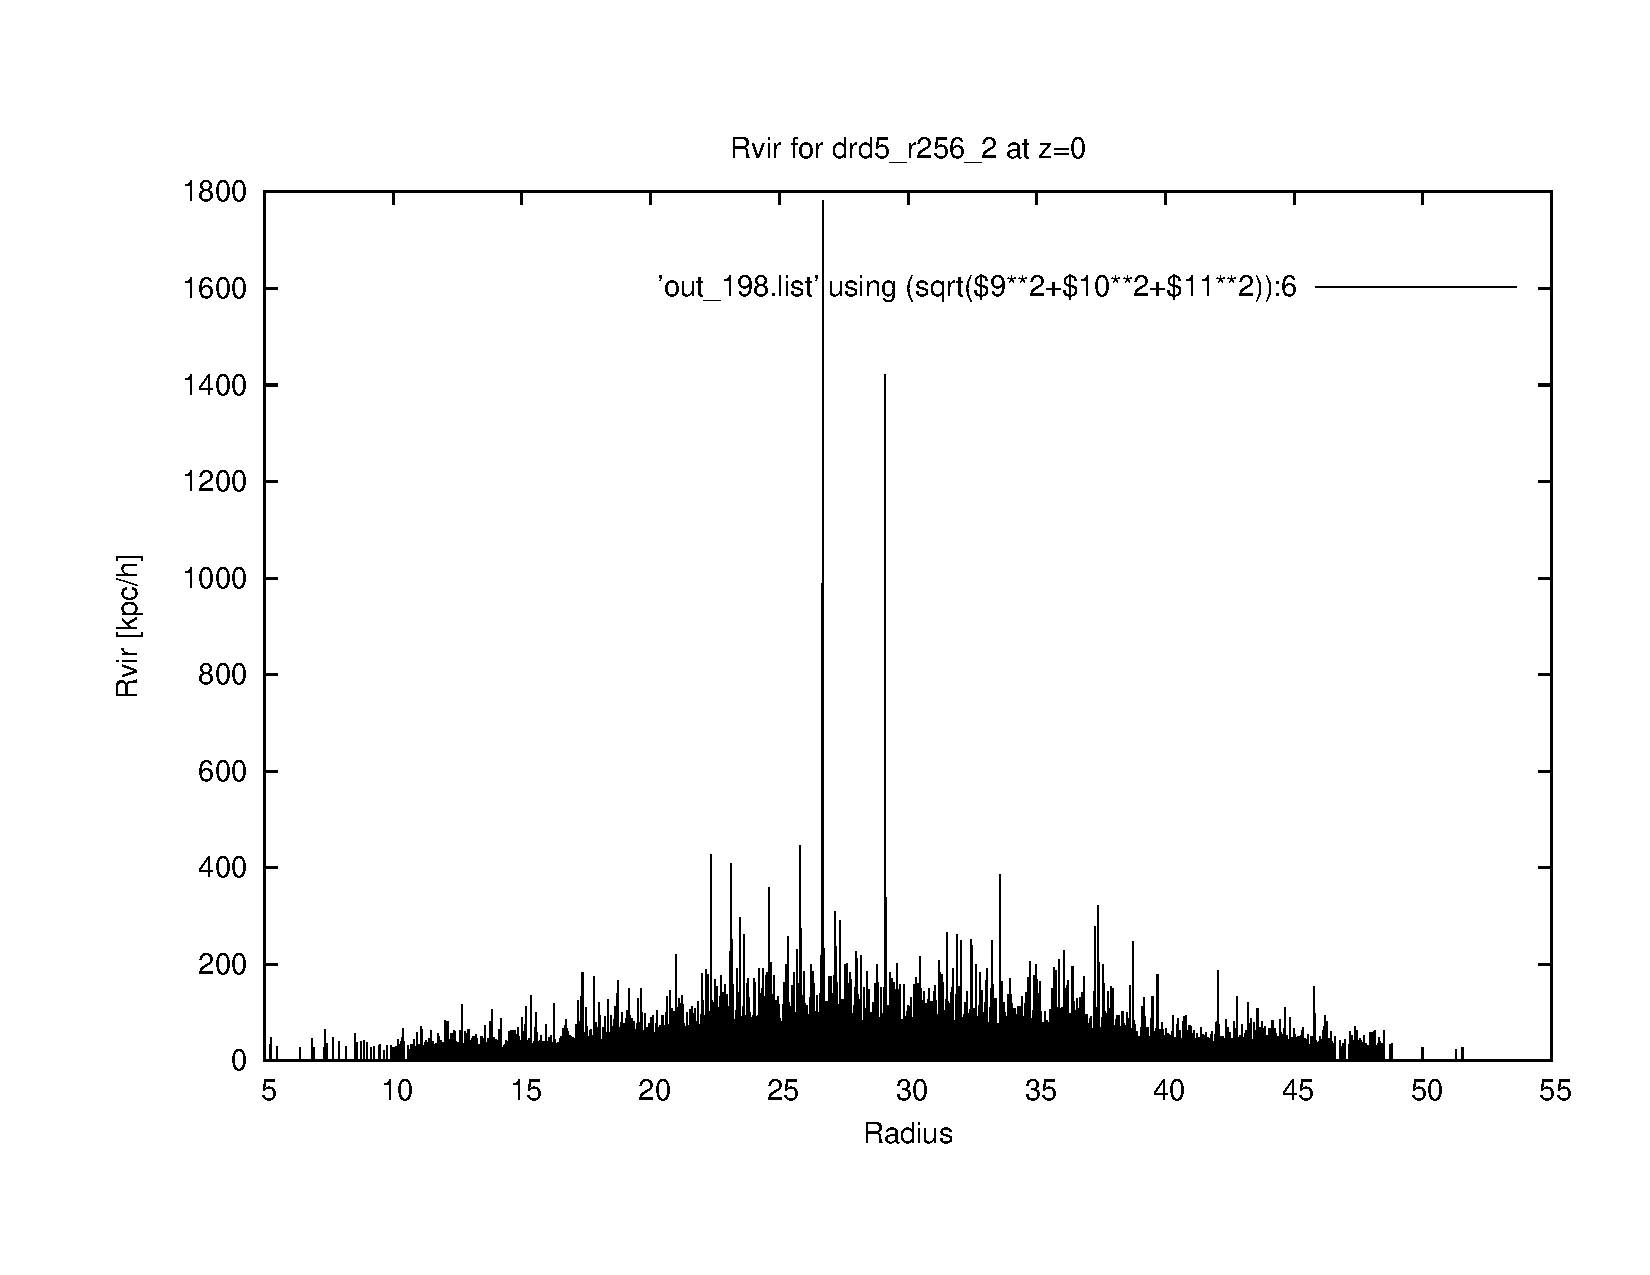
\includegraphics[scale=0.3]{drd5_r256_2/plot_rvir_z0.pdf}
% 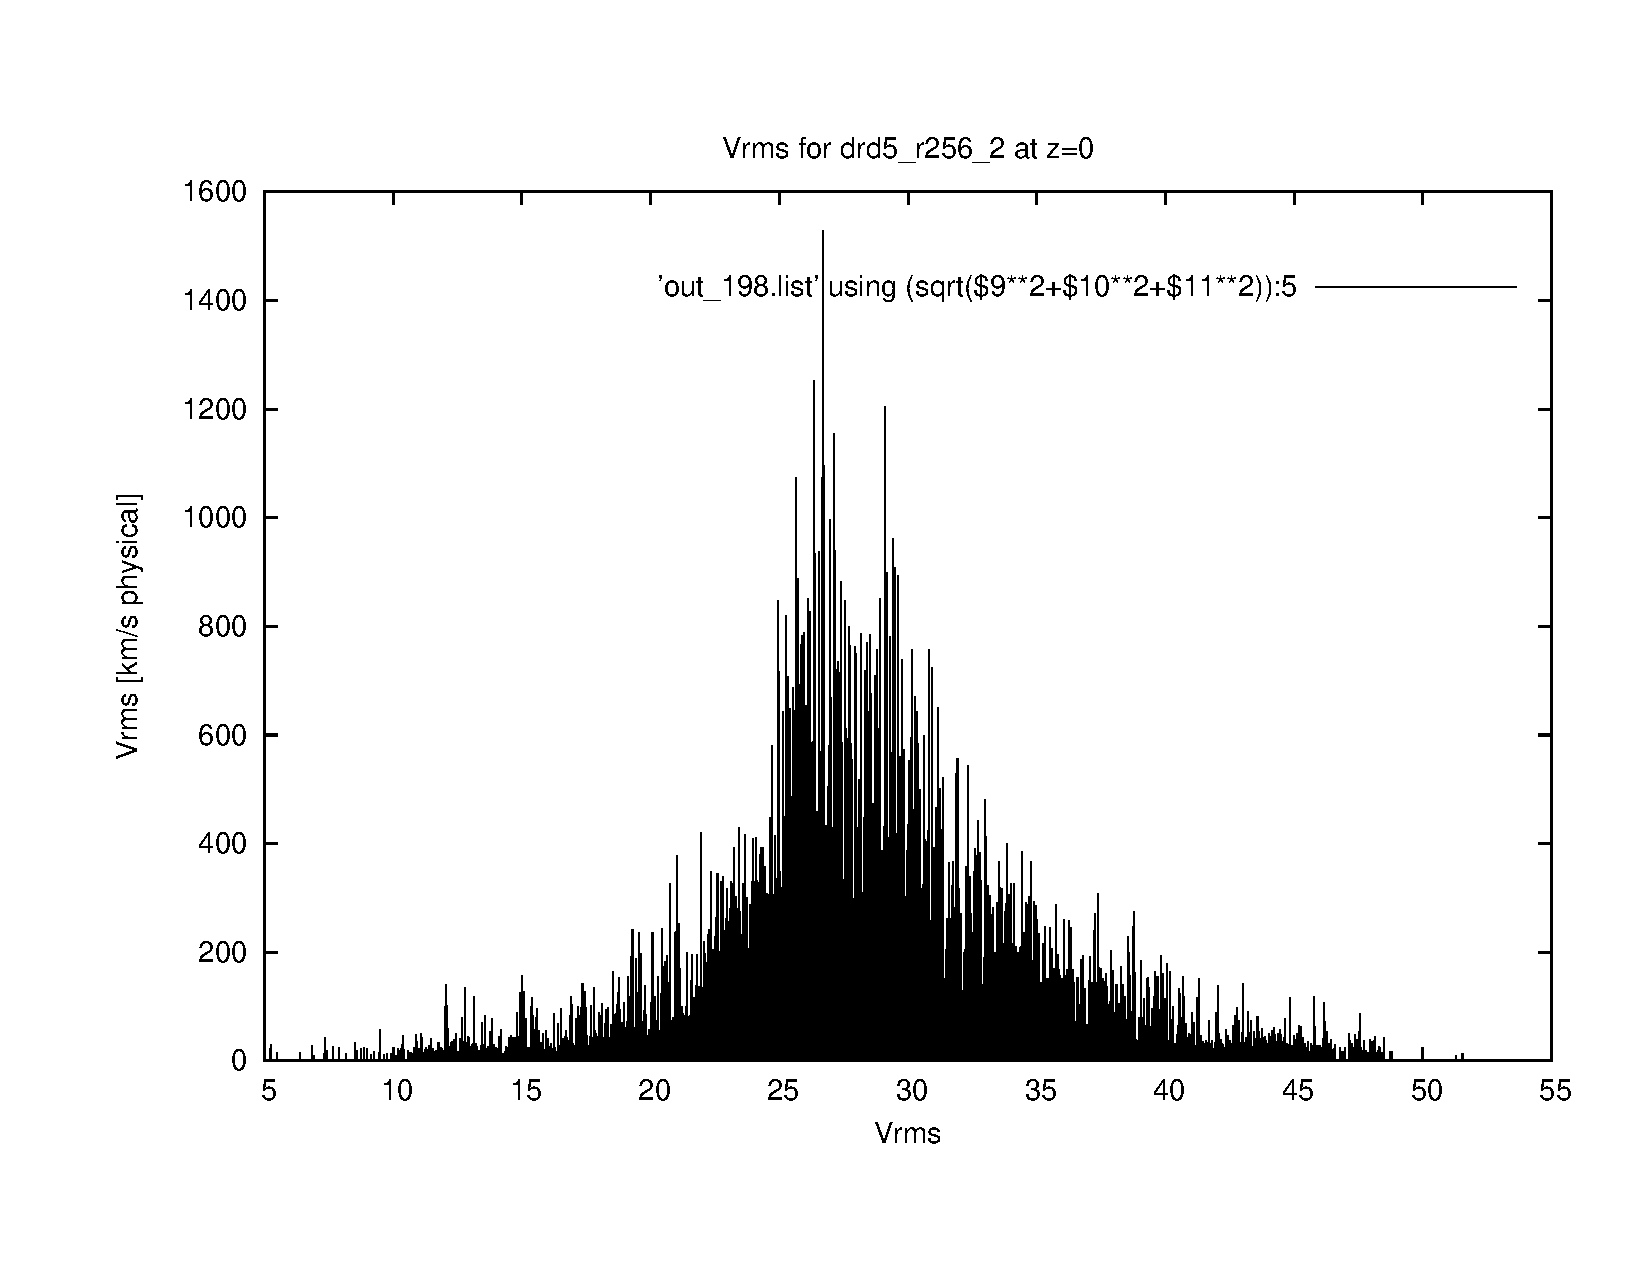
\includegraphics[scale=0.3]{drd5_r256_2/plot_vrms_z0.pdf}

\textsc{galacticussed} $\surd$ \\
$\rightarrow$ fixed in revision 709 \\
$\rightarrow$  not fixed! E-Mail to Andrew \\
After fix in rev. 708 $\rightarrow$ is being re-galacticussed \\
$\rightarrow$ DUMP IT ? \\
$\rightarrow$ gadgetviewer: simulation has "artificial" cross 
galacticus running on SGE \\
$\rightarrow$ re-converted with bugfixed converter (v0.3) \\
is being galacticussed $\rightarrow$ job seems to run! \\
\begin{verbatim}
no: A fatal error occurred! Backtrace for this error:
#0  0x2B3F2E65E897
#1  0x2B3F2E65EE4E
#2  0x301763648F
#3  0x487AA0 in __merger_tree_read_MOD_build_descendent_pointers
#4  0x48ADC3 in __merger_tree_read_MOD_merger_tree_read_do
#5  0x48205E in __merger_tree_construction_MOD_merger_tree_create
#6  0x46F469 in __galacticus_tasks_evolve_tree_MOD_galacticus_task_evolve_tree._omp_fn.0 at galacticus.tasks.evolve_tree
.F90:0
#7  0x46F9C4 in __galacticus_tasks_evolve_tree_MOD_galacticus_task_evolve_tree
#8  0x46FA4F in __galacticus_tasks_MOD_galacticus_task_do
#9  0x4600E4 in MAIN__ at Galacticus.F90:0
\end{verbatim}
\textsc{consistenttreed} $\surd$ \\ 
\textsc{rockstarred} $\surd$ (lasted about 9000minutes) \\

% 
%
%
%
%
%
%
%


\newpage
\subsection{drdx\_3\_r256}

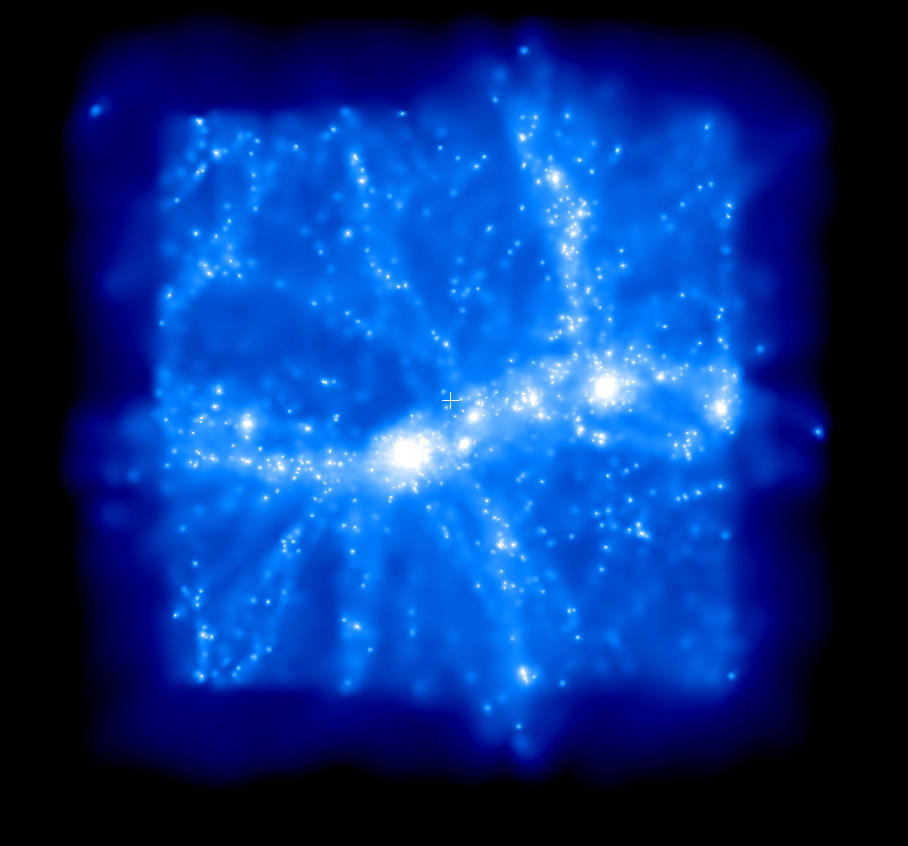
\includegraphics[scale=0.2]{drdx_3_r256/1.png} 
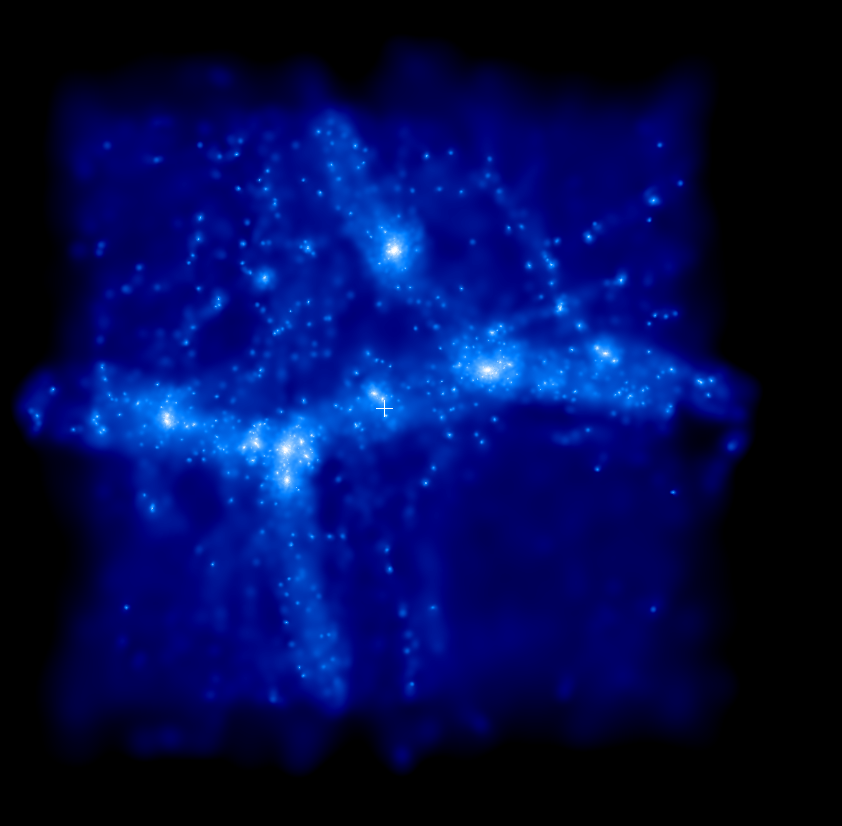
\includegraphics[scale=0.2]{drdx_3_r256/2.png} \\
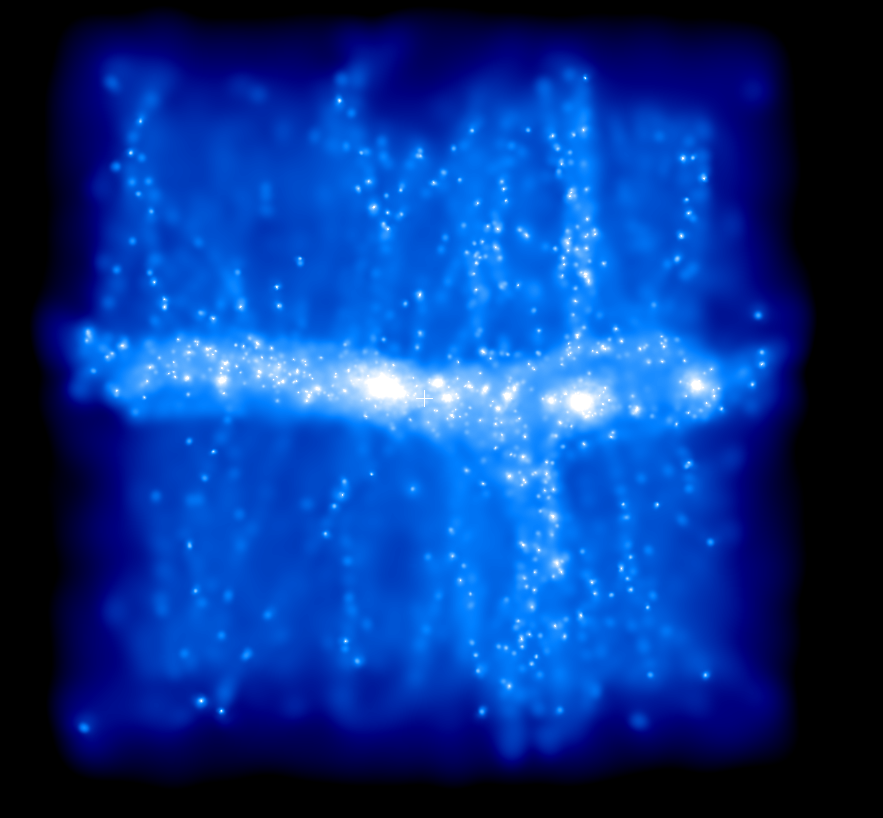
\includegraphics[scale=0.2]{drdx_3_r256/4.png} 
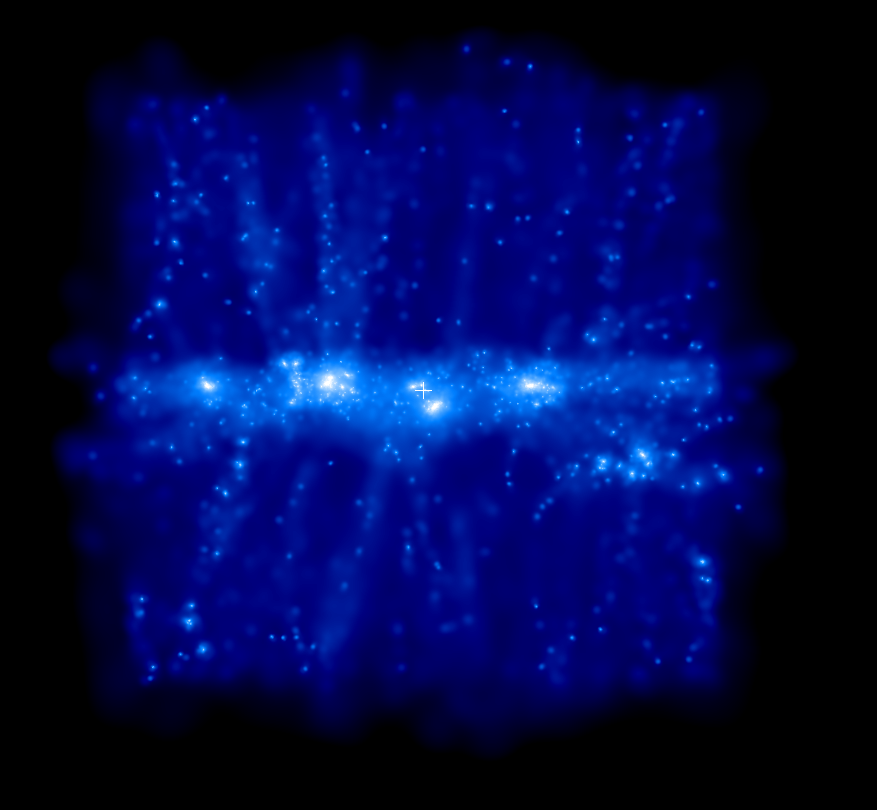
\includegraphics[scale=0.2]{drdx_3_r256/3.png}  \\

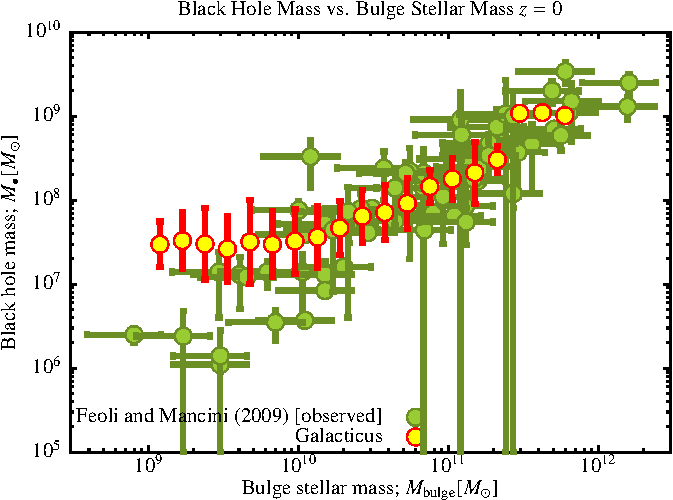
\includegraphics[scale=0.6]{drdx_3_r256/Plot_Black_Hole_vs_Bulge_Mass.pdf}
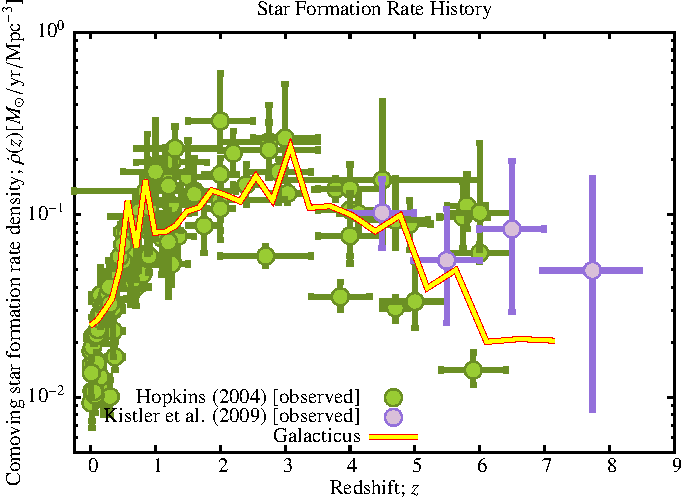
\includegraphics[scale=0.6]{drdx_3_r256/Plot_Star_Formation_History.pdf}
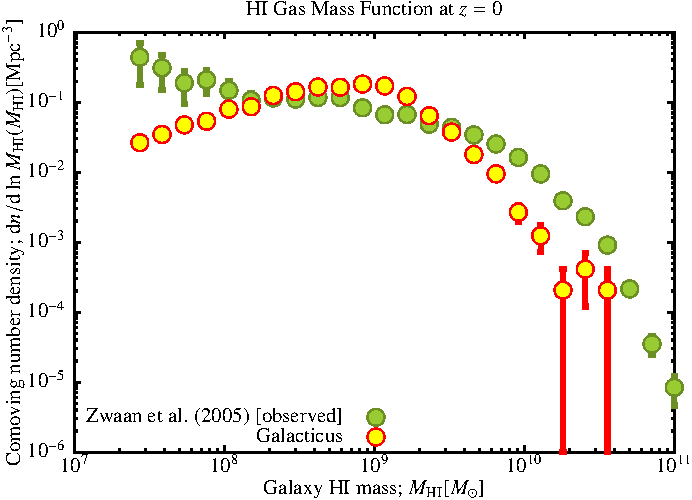
\includegraphics[scale=0.6]{drdx_3_r256/Plot_HI_Mass_Function.pdf}

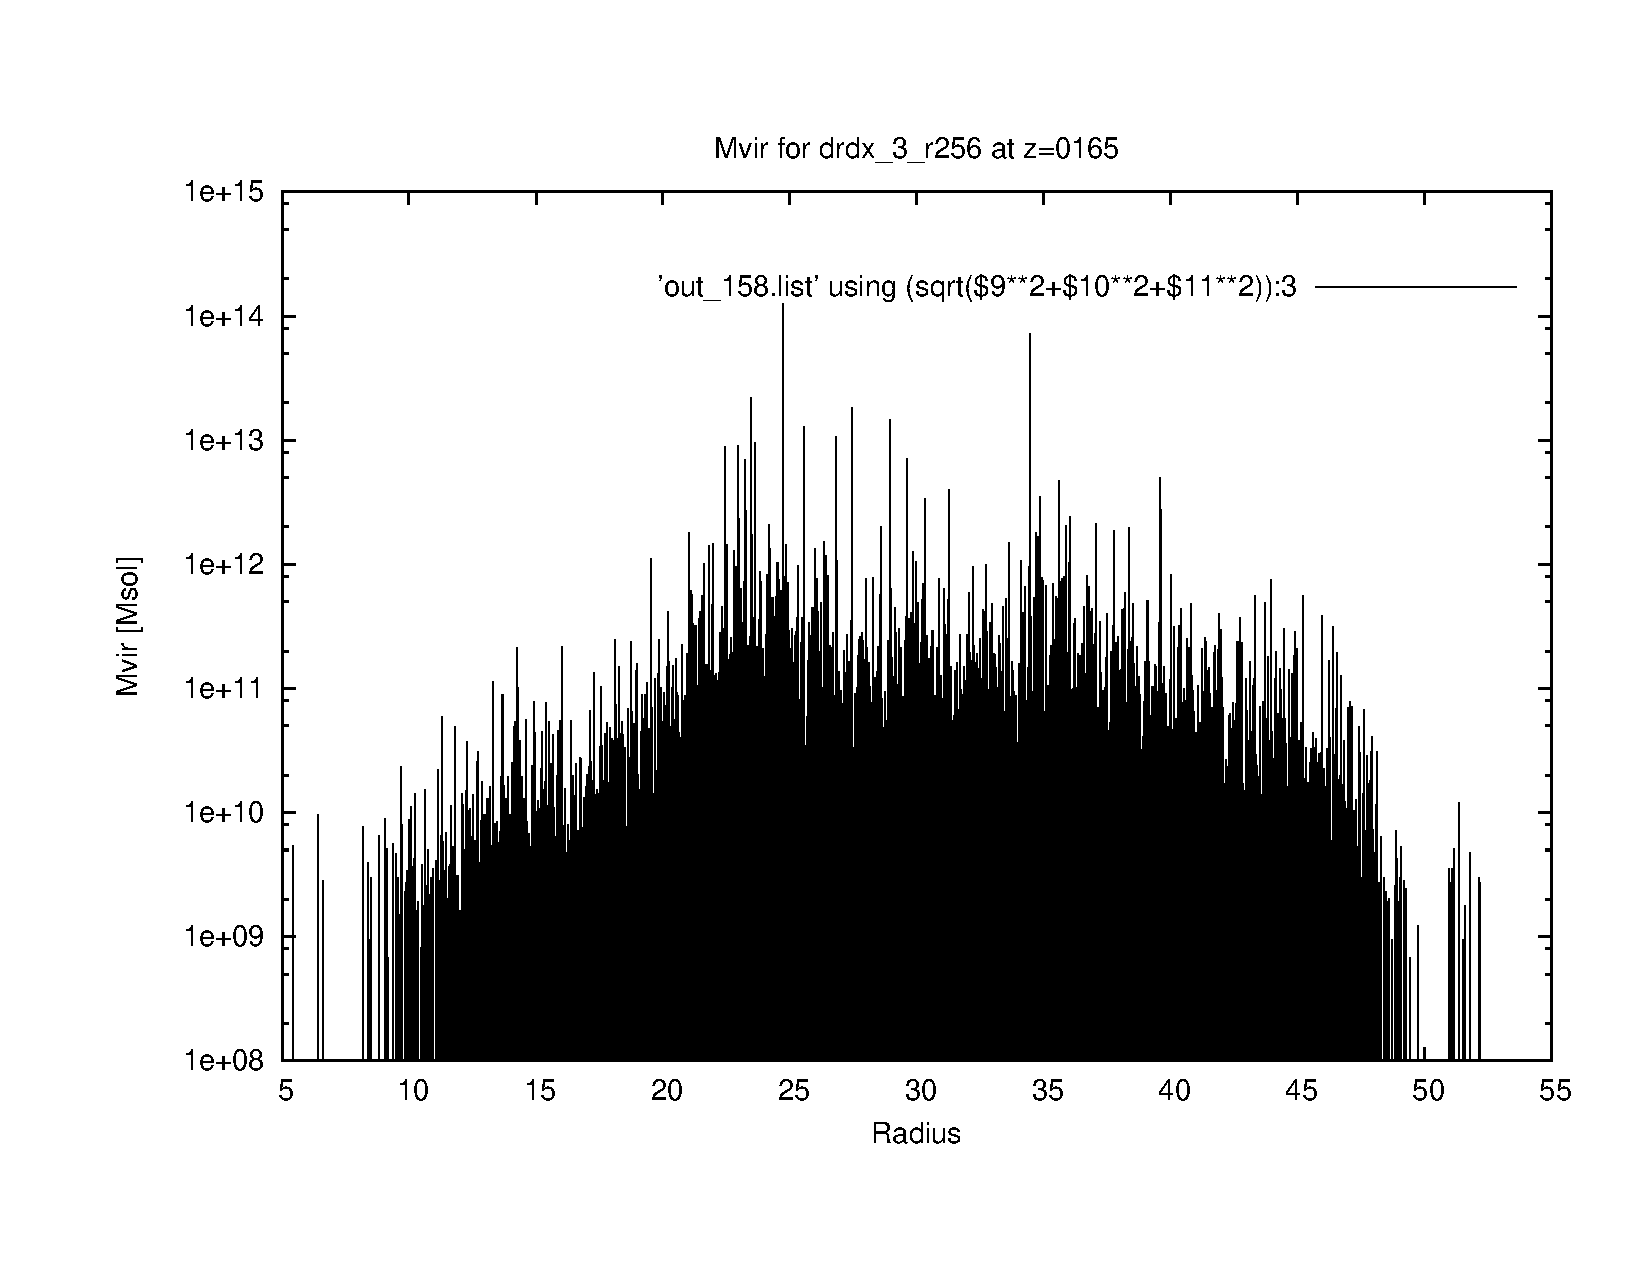
\includegraphics[scale=0.3]{drdx_3_r256/plot_mvir_z0165.pdf}
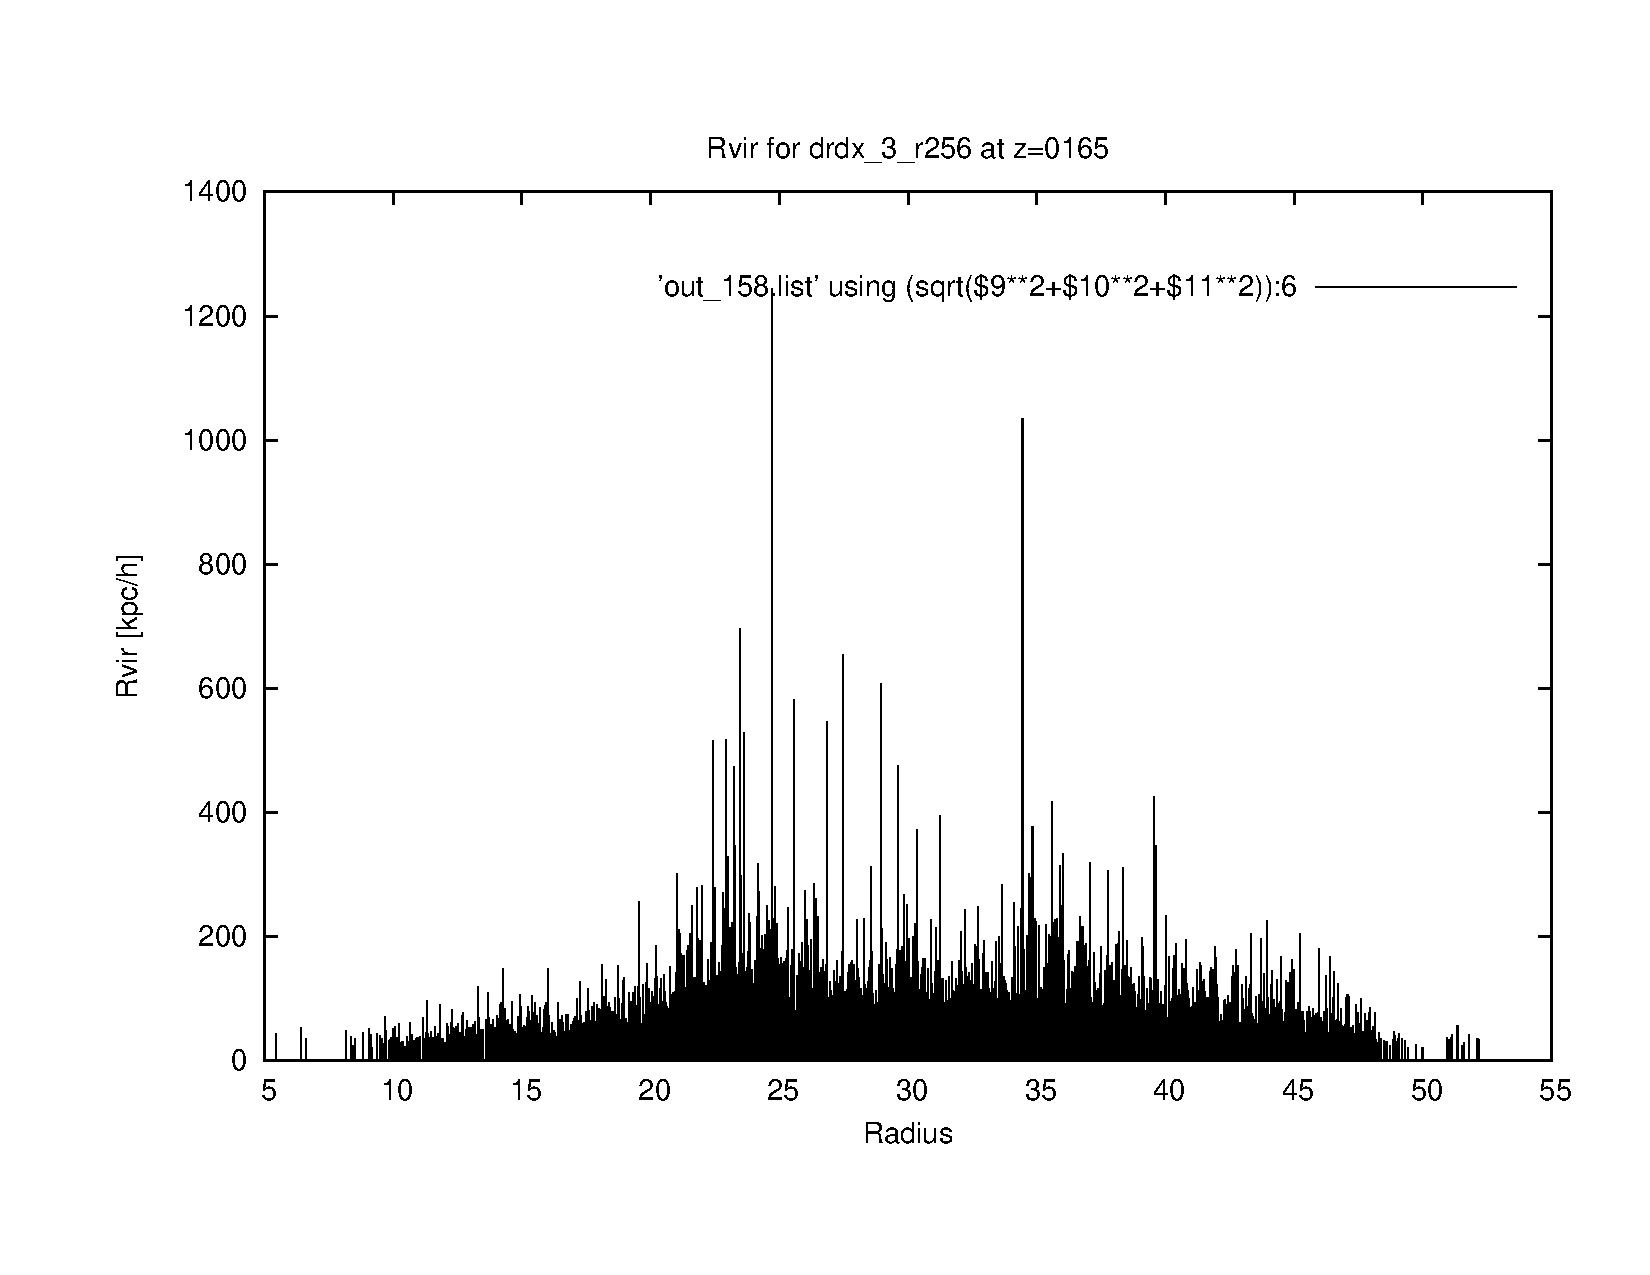
\includegraphics[scale=0.3]{drdx_3_r256/plot_rvir_z0165.pdf}
% \includegraphics[scale=0.3]{drdx_3_r256/plot_vrms_z0165.pdf} 
\includegraphics[scale=0.3]{drdx_3_r256/plot_mvir_z0.pdf}
\includegraphics[scale=0.3]{drdx_3_r256/plot_rvir_z0.pdf}
% \includegraphics[scale=0.3]{drdx_3_r256/plot_vrms_z0.pdf}

\textsc{galacticussed} $\surd$ \\
$\rightarrow$ fixed in revision 709 \\

\textsc{galacticus rev708:} \\
\begin{verbatim}
#4  0x301763648F
#5  0x49B1B8 in __merger_tree_read_MOD_build_descendent_pointers at merger_trees.construct.read.F90:1116
#6  0x49FF70 in __merger_tree_read_MOD_merger_tree_read_do at merger_trees.construct.read.F90:767
#7  0x4923BE in __merger_tree_construction_MOD_merger_tree_create at merger_trees.construct.F90:136
#8  0x4800C6 in __galacticus_tasks_evolve_tree_MOD_galacticus_task_evolve_tree._omp_fn.0 at galacticus.tasks.evolve_tree.F90:169
#9  0x2AC099B4F829
#10  0x3017A07CD0
#11  0x30176DFD3C
#12  0xFFFFFFFFFFFFFFFF
/sge-root/sge/AMD64/spool/astro13/job_scripts/83594: line 22: 13318 Aborted                 (core dumped) ./Galacticus.exe drdx_3_r256.xml
\end{verbatim}
\textsc{consistenttreed} $\surd$ \\
\textsc{rockstarred} $\surd$ \\
is being rockstarred on \texttt{astro-x4600-03} \\
This run is a test if r256 and r128 (\texttt{drdx\_3}) 
are comparable $\rightarrow$ see pictures. \\
	
% 
%
%
%
%
%
%
%


\newpage
\subsection{fuenfincr256\_1}

\includegraphics[scale=0.2]{fuenfincr256_1/1.png} 
\includegraphics[scale=0.2]{fuenfincr256_1/2.png}

\includegraphics[scale=0.6]{fuenfincr256_1/Plot_Black_Hole_vs_Bulge_Mass.pdf}
\includegraphics[scale=0.6]{fuenfincr256_1/Plot_Star_Formation_History.pdf}
\includegraphics[scale=0.6]{fuenfincr256_1/Plot_HI_Mass_Function.pdf}

\includegraphics[scale=0.3]{fuenfincr256_1/plot_mvir_z0165.pdf}
\includegraphics[scale=0.3]{fuenfincr256_1/plot_rvir_z0165.pdf}
% \includegraphics[scale=0.3]{fuenfincr256_1/plot_vrms_z0165.pdf} 
\includegraphics[scale=0.3]{fuenfincr256_1/plot_mvir_z0.pdf}
\includegraphics[scale=0.3]{fuenfincr256_1/plot_rvir_z0.pdf}
% \includegraphics[scale=0.3]{fuenfincr256_1/plot_vrms_z0.pdf}

\textsc{galacticussed} $\surd$ \\
$\rightarrow$ re-galacticussing with rev708 \\
\textsc{galacticus:} rev707 exited without error but not finished \\
\textsc{galacticussed} $\surd$
BUT: 
\begin{verbatim}
[3:46:48 PM CEST] Markus Haider: der fuenfincr256_1 hat a problem
[3:46:52 PM CEST] Markus Haider: der hat keine output gruppe
[3:46:58 PM CEST] Markus Haider: also keinen output
[3:47:30 PM CEST] Markus Haider: btw schon einen output
[3:47:34 PM CEST] Markus Haider: aber es scheint was zu fehlen
\end{verbatim}
$\rightarrow$ E-Mail to Andrew \\
$\rightarrow$ re-converted with bugfixed converter \\
\begin{verbatim}
 Running model....... 
  Reading data for metallicity log10(Z/Z_Solar) = 0.198
   Found 188 ages in the file
  Found 1963 wavelengths in the file
gsl: ../../../../roots/brent.c:57: ERROR: function value is not finite
Default GSL error handler invoked.
\end{verbatim}
tree copied to markus transfer \\
\\ \textsc{galacticus}: 
\begin{verbatim}
Fatal error in Build_Descendent_Pointers():
failed to find descendent node: 12048576 of 12014628
galacticus.sh: line 67:  5751 Aborted  
\end{verbatim}
\textsc{rockstarred} $\surd$ \\ \textsc{consistenttreed} $\surd$

% 
%
%
%
%
%
%
%


\newpage
\subsection{fuenfincr256\_2 $\rightarrow$ dump!}

\includegraphics[scale=0.12]{fuenfincr256_2/1.png} 
\includegraphics[scale=0.12]{fuenfincr256_2/2.png}

\includegraphics[scale=0.6]{fuenfincr256_2/Plot_Black_Hole_vs_Bulge_Mass.pdf}
\includegraphics[scale=0.6]{fuenfincr256_2/Plot_Star_Formation_History.pdf}
\includegraphics[scale=0.6]{fuenfincr256_2/Plot_HI_Mass_Function.pdf}

\includegraphics[scale=0.3]{fuenfincr256_2/plot_mvir_z0165.pdf}
\includegraphics[scale=0.3]{fuenfincr256_2/plot_rvir_z0165.pdf}
% \includegraphics[scale=0.3]{fuenfincr256_2/plot_vrms_z0165.pdf} 
\includegraphics[scale=0.3]{fuenfincr256_2/plot_mvir_z0.pdf}
\includegraphics[scale=0.3]{fuenfincr256_2/plot_rvir_z0.pdf}
% \includegraphics[scale=0.3]{fuenfincr256_2/plot_vrms_z0.pdf}

\textsc{galacticussed} $\surd$
$\rightarrow$ gadgetviewer: simulation has "artificial" cross on right upper corner $\rightarrow$ DUMP IT ? \\
$\rightarrow$ re-converted with bugfixed converter (v0.3) \\
galacticus running on SGE \\
is being galacticussed $\rightarrow$ job seems to run! \\
 \textsc{galacticus}:
 \begin{verbatim}
Fatal error in Build_Descendent_Pointers():
failed to find descendent node 
\end{verbatim}
\textsc{consistenttreed} $\surd$ \\ 
\textsc{rockstarred} $\surd$ (lasted about 9000minutes) \\

% 
%
%
%
%
%
%
%



\newpage
\subsection{gendrkl1r2\_1c\_1}

\includegraphics[scale=0.2]{gendrkl1r2_1c_1/1.png} \\
\includegraphics[scale=0.2]{gendrkl1r2_1c_1/2.png} 

\includegraphics[scale=0.6]{gendrkl1r2_1c_1/Plot_Black_Hole_vs_Bulge_Mass.pdf}
\includegraphics[scale=0.6]{gendrkl1r2_1c_1/Plot_Star_Formation_History.pdf}
\includegraphics[scale=0.6]{gendrkl1r2_1c_1/Plot_HI_Mass_Function.pdf}

\includegraphics[scale=0.3]{gendrkl1r2_1c_1/plot_mvir_z0165.pdf}
\includegraphics[scale=0.3]{gendrkl1r2_1c_1/plot_rvir_z0165.pdf}
% \includegraphics[scale=0.3]{gendrkl1r2_1c_1/plot_vrms_z0165.pdf} 
\includegraphics[scale=0.3]{gendrkl1r2_1c_1/plot_mvir_z0.pdf}
\includegraphics[scale=0.3]{gendrkl1r2_1c_1/plot_rvir_z0.pdf}
% \includegraphics[scale=0.3]{gendrkl1r2_1c_1/plot_vrms_z0.pdf}

\textsc{galacticussed with revision 709} $\surd$
\textsc{consistenttreed} $\surd$ \\ 
\textsc{rockstarred} $\surd$

is being rockstarred on \texttt{astro-x4600-03} \\

E-Mail sent to Bertschinger \\

\begin{verbatim}
$ diff drkt+3c+sl5_1+r2/constraints_drkt+3c+sl5_1+r2.f 
r128/h100/gendrkl1_1c_1/constraints_gendrkl1_1c_1.f 
\end{verbatim}
\begin{verbatim}
$ diff gendrkl1r2_1c_1/grafic_inc_gendrkl1r2_1c_1.f  
r128/h100/gendrkl1_1c_1/grafic_inc_gendrkl1_1c_1.f 
5c5
< 	parameter (np1=256,np2=256,np3=256,ncon=1)
---
> 	parameter (np1=128,np2=128,np3=128,ncon=1)
\end{verbatim}

\begin{verbatim}
diff gendrkl1r2_1c_1/graficIO_gendrkl1r2_1c_1.out r128/h100/gendrkl1_1c_1/graficIO_gendrkl1_1c_1.out 
23c23
<  Particle lattice size: np1,np2,np3=         256         256         256
---
>  Particle lattice size: np1,np2,np3=         128         128         128
25,27c25,27
<  chosen:  0.12500000       0.0000000      5.00000007E-02
<  npart, L_x, L_y, L_z= 16777216    32.00    32.00    32.00 Mpc
<  Particle mass= .1447E+09 solar masses
---
>  chosen:  0.25000000       0.0000000      5.00000007E-02
>  npart, L_x, L_y, L_z=  2097152    32.00    32.00    32.00 Mpc
>  Particle mass= .1158E+10 solar masses
37c37
<           ak,akmax=   16.100662       16.000005475554534     
---
>           ak,akmax=   16.068306       16.000005475554534     
40,41c40,41
<       Mean sigma_delta, sigma_psi=   4.8100653       4.7177238      Mpc
<       Chisq, dof, nu=   16781832.        16777215  0.79710007    
---
>       Mean sigma_delta, sigma_psi=   4.1531582       4.7162638      Mpc
>       Chisq, dof, nu=   2095840.0         2097151 -0.64012647    
43c43
<  Constraint   1:  Sampled, desired= 0.28453870E-02 0.25000000E-01
---
>  Constraint   1:  Sampled, desired=-0.64672055E-02 0.25000000E-01
46c46
<       Sampled, desired=  0.21657717       16.718990    
---
>       Sampled, desired=   1.1184790       16.713776    
49c49
<  Constraint   1:  Final= 0.25000000E-01
---
>  Constraint   1:  Final= 0.25000002E-01
52,54c52,54
<       sigma_delta, sigma_psi=   4.9692168       7.6522889      Mpc
<       Chisq, dof=   16781832.        16777214
<       Maximum delta, displacement=   27.548712       17.026833      Mpc
---
>       sigma_delta, sigma_psi=   4.2376528       6.6093922      Mpc
>       Chisq, dof=   2095838.9         2097150
>       Maximum delta, displacement=   22.542503       14.168747      Mpc
56c56
<  Scaling density and displacements to a=  2.75129788E-02
---
>  Scaling density and displacements to a=  3.36233079E-02
58,59c58,59
<  For a=astart: linear sigma, delmax=  0.18037927      0.99999994    
<  RMS, max. 3-D displacement=  0.27777302      0.61806273      Mpc
---
>  For a=astart: linear sigma, delmax=  0.18798503       1.0000000    
>  RMS, max. 3-D displacement=  0.29319692      0.62853473      Mpc

\end{verbatim}

This run is a test if r256 and r128 (\texttt{gendrkl\_1c\_1}) are comparable $\rightarrow$ see pictures. Sims are not only different in resolution! 

% 
%
%
%
%
%
%
%


\newpage
\subsection{NGenIC\_26214}

\includegraphics[scale=0.1]{NGenIC_26214/50.jpg} 
\includegraphics[scale=0.1]{NGenIC_26214/100.jpg}  \\

\includegraphics[scale=0.1]{NGenIC_26214/150.jpg} 
\includegraphics[scale=0.1]{NGenIC_26214/200.jpg}  \\

\includegraphics[scale=0.1]{NGenIC_26214/rotate_00074.jpg} 
\includegraphics[scale=0.1]{NGenIC_26214/rotate_00131.jpg}

is being rockstarred  \\

% 
%
%
%
%
%
%
%

\newpage
\subsection{stages\_07}

% \includegraphics[scale=0.1]{stages_07/50.jpg} 
% \includegraphics[scale=0.1]{stages_07/100.jpg}  \\
% 
% \includegraphics[scale=0.1]{stages_07/150.jpg} 
% \includegraphics[scale=0.1]{stages_07/199.jpg}  \\
% 
% \includegraphics[scale=0.1]{stages_07/rotate_00074.jpg} 
% \includegraphics[scale=0.1]{stages_07/rotate_00131.jpg}

\includegraphics[scale=0.3]{stages_07/plot_mvir_z0165.pdf}
\includegraphics[scale=0.3]{stages_07/plot_rvir_z0165.pdf}
% \includegraphics[scale=0.3]{stages_07/plot_vrms_z0165.pdf} 
\includegraphics[scale=0.3]{stages_07/plot_mvir_z0.pdf}
\includegraphics[scale=0.3]{stages_07/plot_rvir_z0.pdf}
% \includegraphics[scale=0.3]{stages_07/plot_vrms_z0.pdf}

is being rockstarred  \\
 
% 
%
%
%
%
%
%
%

\newpage
\subsection{stages\_12}

\includegraphics[scale=0.1]{stages_12/50.jpg} 
\includegraphics[scale=0.1]{stages_12/100.jpg}  \\

\includegraphics[scale=0.1]{stages_12/150.jpg} 
\includegraphics[scale=0.1]{stages_12/199.jpg}  \\

\includegraphics[scale=0.1]{stages_12/rotate_00074.jpg} 
\includegraphics[scale=0.1]{stages_12/rotate_00131.jpg}

\includegraphics[scale=0.3]{stages_12/plot_mvir_z0165.pdf}
\includegraphics[scale=0.3]{stages_12/plot_rvir_z0165.pdf}
% \includegraphics[scale=0.3]{stages_12/plot_vrms_z0165.pdf} 
\includegraphics[scale=0.3]{stages_12/plot_mvir_z0.pdf}
\includegraphics[scale=0.3]{stages_12/plot_rvir_z0.pdf}
% \includegraphics[scale=0.3]{stages_12/plot_vrms_z0.pdf}

galacticus strange error: 
\begin{verbatim}
Fatal error in Cosmology_Age_Matter_Lambda():
expansion factor is invalid
\end{verbatim}
is being galacticussed \\
\textsc{consistenttreed} $\surd$ \\ 
\textsc{rockstarred} $\surd$

% 
%
%
%
%
%
%
%

\newpage
\subsection{stages\_13}

\includegraphics[scale=0.1]{stages_13/50.jpg} 
\includegraphics[scale=0.1]{stages_13/100.jpg}  \\

\includegraphics[scale=0.1]{stages_13/150.jpg} 
\includegraphics[scale=0.1]{stages_13/199.jpg}  \\

\includegraphics[scale=0.1]{stages_13/rotate_00074.jpg} 
\includegraphics[scale=0.1]{stages_13/rotate_00131.jpg}

\includegraphics[scale=0.3]{stages_13/plot_mvir_z0165.pdf}
\includegraphics[scale=0.3]{stages_13/plot_rvir_z0165.pdf}
% \includegraphics[scale=0.3]{stages_13/plot_vrms_z0165.pdf} 
\includegraphics[scale=0.3]{stages_13/plot_mvir_z0.pdf}
\includegraphics[scale=0.3]{stages_13/plot_rvir_z0.pdf}
% \includegraphics[scale=0.3]{stages_13/plot_vrms_z0.pdf}

galacticus strange error: 
\begin{verbatim}
Fatal error in Cosmology_Age_Matter_Lambda():
expansion factor is invalid
\end{verbatim}
is being galacticussed \\
\textsc{consistenttreed} $\surd$ \\ 
\textsc{rockstarred} $\surd$

% 
%
%
%
%
%
%
%


\newpage
\subsection{stages\_14}

\includegraphics[scale=0.1]{stages_14/50.jpg} 
\includegraphics[scale=0.1]{stages_14/100.jpg}  \\

\includegraphics[scale=0.1]{stages_14/150.jpg} 
\includegraphics[scale=0.1]{stages_14/199.jpg}  \\

\includegraphics[scale=0.1]{stages_14/rotate_00074.jpg} 
\includegraphics[scale=0.1]{stages_14/rotate_00131.jpg}

is being rockstarred  \\

% 
%
%
%
%
%
%
%

\newpage
\subsection{stages\_18}

\includegraphics[scale=0.1]{stages_18/50.jpg} 
\includegraphics[scale=0.1]{stages_18/100.jpg}  \\

\includegraphics[scale=0.1]{stages_18/150.jpg} 
\includegraphics[scale=0.1]{stages_18/199.jpg}  \\

\includegraphics[scale=0.1]{stages_18/rotate_00074.jpg} 
\includegraphics[scale=0.1]{stages_18/rotate_00131.jpg}

is being rockstarred  \\

% 
%
%
%
%
%
%
%

\newpage
\subsection{stages\_19}

\includegraphics[scale=0.1]{stages_19/50.jpg} 
\includegraphics[scale=0.1]{stages_19/100.jpg}  \\

\includegraphics[scale=0.1]{stages_19/150.jpg} 
\includegraphics[scale=0.1]{stages_19/199.jpg}  \\

\includegraphics[scale=0.1]{stages_19/rotate_00074.jpg} 
\includegraphics[scale=0.1]{stages_19/rotate_00131.jpg}


% 
%
%
%
%
%
%
%

\newpage
\subsection{stages\_20}

\includegraphics[scale=0.1]{stages_20/50.jpg} 
\includegraphics[scale=0.1]{stages_20/100.jpg}  \\

\includegraphics[scale=0.1]{stages_20/150.jpg} 
\includegraphics[scale=0.1]{stages_20/199.jpg}  \\

\includegraphics[scale=0.1]{stages_20/rotate_00074.jpg} 
\includegraphics[scale=0.1]{stages_20/rotate_00131.jpg}


% 
%
%
%
%
%
%
%


\newpage
\subsection{stages\_21}

\includegraphics[scale=0.1]{stages_21/50.jpg} 
\includegraphics[scale=0.1]{stages_21/100.jpg}  \\

\includegraphics[scale=0.1]{stages_21/150.jpg} 
\includegraphics[scale=0.1]{stages_21/199.jpg}  \\

\includegraphics[scale=0.1]{stages_21/rotate_00074.jpg} 
\includegraphics[scale=0.1]{stages_21/rotate_00131.jpg}  \\

is being rockstarred \\
